\PassOptionsToPackage{unicode=true}{hyperref} % options for packages loaded elsewhere
\PassOptionsToPackage{hyphens}{url}
%
\documentclass[]{article}
\usepackage{lmodern}
\usepackage{amssymb,amsmath}
\usepackage{ifxetex,ifluatex}
\usepackage{fixltx2e} % provides \textsubscript
\ifnum 0\ifxetex 1\fi\ifluatex 1\fi=0 % if pdftex
  \usepackage[T1]{fontenc}
  \usepackage[utf8]{inputenc}
  \usepackage{textcomp} % provides euro and other symbols
\else % if luatex or xelatex
  \usepackage{unicode-math}
  \defaultfontfeatures{Ligatures=TeX,Scale=MatchLowercase}
\fi
% use upquote if available, for straight quotes in verbatim environments
\IfFileExists{upquote.sty}{\usepackage{upquote}}{}
% use microtype if available
\IfFileExists{microtype.sty}{%
\usepackage[]{microtype}
\UseMicrotypeSet[protrusion]{basicmath} % disable protrusion for tt fonts
}{}
\IfFileExists{parskip.sty}{%
\usepackage{parskip}
}{% else
\setlength{\parindent}{0pt}
\setlength{\parskip}{6pt plus 2pt minus 1pt}
}
\usepackage{hyperref}
\hypersetup{
            pdftitle={Final Project EDA},
            pdfborder={0 0 0},
            breaklinks=true}
\urlstyle{same}  % don't use monospace font for urls
\usepackage[margin=1in]{geometry}
\usepackage{color}
\usepackage{fancyvrb}
\newcommand{\VerbBar}{|}
\newcommand{\VERB}{\Verb[commandchars=\\\{\}]}
\DefineVerbatimEnvironment{Highlighting}{Verbatim}{commandchars=\\\{\}}
% Add ',fontsize=\small' for more characters per line
\usepackage{framed}
\definecolor{shadecolor}{RGB}{248,248,248}
\newenvironment{Shaded}{\begin{snugshade}}{\end{snugshade}}
\newcommand{\AlertTok}[1]{\textcolor[rgb]{0.94,0.16,0.16}{#1}}
\newcommand{\AnnotationTok}[1]{\textcolor[rgb]{0.56,0.35,0.01}{\textbf{\textit{#1}}}}
\newcommand{\AttributeTok}[1]{\textcolor[rgb]{0.77,0.63,0.00}{#1}}
\newcommand{\BaseNTok}[1]{\textcolor[rgb]{0.00,0.00,0.81}{#1}}
\newcommand{\BuiltInTok}[1]{#1}
\newcommand{\CharTok}[1]{\textcolor[rgb]{0.31,0.60,0.02}{#1}}
\newcommand{\CommentTok}[1]{\textcolor[rgb]{0.56,0.35,0.01}{\textit{#1}}}
\newcommand{\CommentVarTok}[1]{\textcolor[rgb]{0.56,0.35,0.01}{\textbf{\textit{#1}}}}
\newcommand{\ConstantTok}[1]{\textcolor[rgb]{0.00,0.00,0.00}{#1}}
\newcommand{\ControlFlowTok}[1]{\textcolor[rgb]{0.13,0.29,0.53}{\textbf{#1}}}
\newcommand{\DataTypeTok}[1]{\textcolor[rgb]{0.13,0.29,0.53}{#1}}
\newcommand{\DecValTok}[1]{\textcolor[rgb]{0.00,0.00,0.81}{#1}}
\newcommand{\DocumentationTok}[1]{\textcolor[rgb]{0.56,0.35,0.01}{\textbf{\textit{#1}}}}
\newcommand{\ErrorTok}[1]{\textcolor[rgb]{0.64,0.00,0.00}{\textbf{#1}}}
\newcommand{\ExtensionTok}[1]{#1}
\newcommand{\FloatTok}[1]{\textcolor[rgb]{0.00,0.00,0.81}{#1}}
\newcommand{\FunctionTok}[1]{\textcolor[rgb]{0.00,0.00,0.00}{#1}}
\newcommand{\ImportTok}[1]{#1}
\newcommand{\InformationTok}[1]{\textcolor[rgb]{0.56,0.35,0.01}{\textbf{\textit{#1}}}}
\newcommand{\KeywordTok}[1]{\textcolor[rgb]{0.13,0.29,0.53}{\textbf{#1}}}
\newcommand{\NormalTok}[1]{#1}
\newcommand{\OperatorTok}[1]{\textcolor[rgb]{0.81,0.36,0.00}{\textbf{#1}}}
\newcommand{\OtherTok}[1]{\textcolor[rgb]{0.56,0.35,0.01}{#1}}
\newcommand{\PreprocessorTok}[1]{\textcolor[rgb]{0.56,0.35,0.01}{\textit{#1}}}
\newcommand{\RegionMarkerTok}[1]{#1}
\newcommand{\SpecialCharTok}[1]{\textcolor[rgb]{0.00,0.00,0.00}{#1}}
\newcommand{\SpecialStringTok}[1]{\textcolor[rgb]{0.31,0.60,0.02}{#1}}
\newcommand{\StringTok}[1]{\textcolor[rgb]{0.31,0.60,0.02}{#1}}
\newcommand{\VariableTok}[1]{\textcolor[rgb]{0.00,0.00,0.00}{#1}}
\newcommand{\VerbatimStringTok}[1]{\textcolor[rgb]{0.31,0.60,0.02}{#1}}
\newcommand{\WarningTok}[1]{\textcolor[rgb]{0.56,0.35,0.01}{\textbf{\textit{#1}}}}
\usepackage{graphicx,grffile}
\makeatletter
\def\maxwidth{\ifdim\Gin@nat@width>\linewidth\linewidth\else\Gin@nat@width\fi}
\def\maxheight{\ifdim\Gin@nat@height>\textheight\textheight\else\Gin@nat@height\fi}
\makeatother
% Scale images if necessary, so that they will not overflow the page
% margins by default, and it is still possible to overwrite the defaults
% using explicit options in \includegraphics[width, height, ...]{}
\setkeys{Gin}{width=\maxwidth,height=\maxheight,keepaspectratio}
\setlength{\emergencystretch}{3em}  % prevent overfull lines
\providecommand{\tightlist}{%
  \setlength{\itemsep}{0pt}\setlength{\parskip}{0pt}}
\setcounter{secnumdepth}{0}
% Redefines (sub)paragraphs to behave more like sections
\ifx\paragraph\undefined\else
\let\oldparagraph\paragraph
\renewcommand{\paragraph}[1]{\oldparagraph{#1}\mbox{}}
\fi
\ifx\subparagraph\undefined\else
\let\oldsubparagraph\subparagraph
\renewcommand{\subparagraph}[1]{\oldsubparagraph{#1}\mbox{}}
\fi

% set default figure placement to htbp
\makeatletter
\def\fps@figure{htbp}
\makeatother

\usepackage{booktabs}
\usepackage{longtable}
\usepackage{array}
\usepackage{multirow}
\usepackage{wrapfig}
\usepackage{float}
\usepackage{colortbl}
\usepackage{pdflscape}
\usepackage{tabu}
\usepackage{threeparttable}
\usepackage{threeparttablex}
\usepackage[normalem]{ulem}
\usepackage{makecell}
\usepackage{xcolor}

\title{Final Project EDA}
\author{}
\date{\vspace{-2.5em}}

\begin{document}
\maketitle

\begin{Shaded}
\begin{Highlighting}[]
\KeywordTok{library}\NormalTok{(mltools)}
\KeywordTok{library}\NormalTok{(data.table)}
\KeywordTok{library}\NormalTok{(dplyr)}
\end{Highlighting}
\end{Shaded}

\begin{verbatim}
## 
## Attaching package: 'dplyr'
\end{verbatim}

\begin{verbatim}
## The following objects are masked from 'package:data.table':
## 
##     between, first, last
\end{verbatim}

\begin{verbatim}
## The following objects are masked from 'package:stats':
## 
##     filter, lag
\end{verbatim}

\begin{verbatim}
## The following objects are masked from 'package:base':
## 
##     intersect, setdiff, setequal, union
\end{verbatim}

\begin{Shaded}
\begin{Highlighting}[]
\KeywordTok{library}\NormalTok{(stringr)}
\KeywordTok{library}\NormalTok{(klaR)}
\end{Highlighting}
\end{Shaded}

\begin{verbatim}
## Loading required package: MASS
\end{verbatim}

\begin{verbatim}
## 
## Attaching package: 'MASS'
\end{verbatim}

\begin{verbatim}
## The following object is masked from 'package:dplyr':
## 
##     select
\end{verbatim}

\begin{Shaded}
\begin{Highlighting}[]
\KeywordTok{library}\NormalTok{(gapminder)}
\KeywordTok{library}\NormalTok{(ggplot2)}
\KeywordTok{library}\NormalTok{(dendextend)}
\end{Highlighting}
\end{Shaded}

\begin{verbatim}
## 
## ---------------------
## Welcome to dendextend version 1.15.2
## Type citation('dendextend') for how to cite the package.
## 
## Type browseVignettes(package = 'dendextend') for the package vignette.
## The github page is: https://github.com/talgalili/dendextend/
## 
## Suggestions and bug-reports can be submitted at: https://github.com/talgalili/dendextend/issues
## You may ask questions at stackoverflow, use the r and dendextend tags: 
##   https://stackoverflow.com/questions/tagged/dendextend
## 
##  To suppress this message use:  suppressPackageStartupMessages(library(dendextend))
## ---------------------
\end{verbatim}

\begin{verbatim}
## 
## Attaching package: 'dendextend'
\end{verbatim}

\begin{verbatim}
## The following object is masked from 'package:data.table':
## 
##     set
\end{verbatim}

\begin{verbatim}
## The following object is masked from 'package:stats':
## 
##     cutree
\end{verbatim}

\begin{Shaded}
\begin{Highlighting}[]
\KeywordTok{library}\NormalTok{(Hmisc)}
\end{Highlighting}
\end{Shaded}

\begin{verbatim}
## Loading required package: lattice
\end{verbatim}

\begin{verbatim}
## Loading required package: survival
\end{verbatim}

\begin{verbatim}
## Loading required package: Formula
\end{verbatim}

\begin{verbatim}
## 
## Attaching package: 'Hmisc'
\end{verbatim}

\begin{verbatim}
## The following objects are masked from 'package:dplyr':
## 
##     src, summarize
\end{verbatim}

\begin{verbatim}
## The following objects are masked from 'package:base':
## 
##     format.pval, units
\end{verbatim}

\begin{Shaded}
\begin{Highlighting}[]
\KeywordTok{library}\NormalTok{(mlbench)}
\KeywordTok{library}\NormalTok{(caret)}
\end{Highlighting}
\end{Shaded}

\begin{verbatim}
## 
## Attaching package: 'caret'
\end{verbatim}

\begin{verbatim}
## The following object is masked from 'package:survival':
## 
##     cluster
\end{verbatim}

\begin{Shaded}
\begin{Highlighting}[]
\KeywordTok{library}\NormalTok{(factoextra)}
\end{Highlighting}
\end{Shaded}

\begin{verbatim}
## Welcome! Want to learn more? See two factoextra-related books at https://goo.gl/ve3WBa
\end{verbatim}

\begin{Shaded}
\begin{Highlighting}[]
\KeywordTok{library}\NormalTok{(NbClust)}
\KeywordTok{library}\NormalTok{(fossil)}
\end{Highlighting}
\end{Shaded}

\begin{verbatim}
## Loading required package: sp
\end{verbatim}

\begin{verbatim}
## Loading required package: maps
\end{verbatim}

\begin{verbatim}
## Loading required package: shapefiles
\end{verbatim}

\begin{verbatim}
## Loading required package: foreign
\end{verbatim}

\begin{verbatim}
## 
## Attaching package: 'shapefiles'
\end{verbatim}

\begin{verbatim}
## The following objects are masked from 'package:foreign':
## 
##     read.dbf, write.dbf
\end{verbatim}

\begin{Shaded}
\begin{Highlighting}[]
\KeywordTok{library}\NormalTok{(countrycode)}
\KeywordTok{library}\NormalTok{(tidyverse)}
\end{Highlighting}
\end{Shaded}

\begin{verbatim}
## -- Attaching packages --------------------------------------- tidyverse 1.3.1 --
\end{verbatim}

\begin{verbatim}
## v tibble  3.1.6     v purrr   0.3.4
## v tidyr   1.2.0     v forcats 0.5.1
## v readr   2.1.2
\end{verbatim}

\begin{verbatim}
## -- Conflicts ------------------------------------------ tidyverse_conflicts() --
## x dplyr::between()    masks data.table::between()
## x dplyr::filter()     masks stats::filter()
## x dplyr::first()      masks data.table::first()
## x dplyr::lag()        masks stats::lag()
## x dplyr::last()       masks data.table::last()
## x purrr::lift()       masks caret::lift()
## x purrr::map()        masks maps::map()
## x tidyr::replace_na() masks mltools::replace_na()
## x MASS::select()      masks dplyr::select()
## x Hmisc::src()        masks dplyr::src()
## x Hmisc::summarize()  masks dplyr::summarize()
## x purrr::transpose()  masks data.table::transpose()
\end{verbatim}

\begin{Shaded}
\begin{Highlighting}[]
\KeywordTok{library}\NormalTok{(ggrepel)}
\KeywordTok{library}\NormalTok{(kableExtra)}
\end{Highlighting}
\end{Shaded}

\begin{verbatim}
## 
## Attaching package: 'kableExtra'
\end{verbatim}

\begin{verbatim}
## The following object is masked from 'package:dplyr':
## 
##     group_rows
\end{verbatim}

\begin{Shaded}
\begin{Highlighting}[]
\NormalTok{data <-}\StringTok{ }\KeywordTok{read.csv}\NormalTok{(}\StringTok{'data/immigration_policies/policy_list.csv'}\NormalTok{)}
\CommentTok{# summary(data)}
\end{Highlighting}
\end{Shaded}

\begin{Shaded}
\begin{Highlighting}[]
\KeywordTok{colSums}\NormalTok{(}\KeywordTok{is.na}\NormalTok{(data))[}\KeywordTok{colSums}\NormalTok{(}\KeywordTok{is.na}\NormalTok{(data)) }\OperatorTok{!=}\StringTok{ }\DecValTok{0}\NormalTok{]}
\end{Highlighting}
\end{Shaded}

\begin{verbatim}
##               ISO2           AIR_TYPE        TARGETS_AIR          LAND_TYPE 
##                  7               1073               1169               1511 
##       TARGETS_LAND           SEA_TYPE        TARGETS_SEA       CITIZEN_LIST 
##               1571               1534               1554               1568 
##   HISTORY_BAN_LIST       REFUGEE_LIST      VISA_BAN_TYPE      VISA_BAN_LIST 
##               1492               1760               1699               1741 
## CITIZEN_EXCEP_LIST COUNTRY_EXCEP_LIST 
##               1390               1625
\end{verbatim}

\begin{Shaded}
\begin{Highlighting}[]
\NormalTok{mod_df <-}\StringTok{ }\KeywordTok{data.frame}\NormalTok{(data)}

\CommentTok{# dropping columns that will not affect our data analysis in any way}
\NormalTok{mod_df <-}\StringTok{ }\NormalTok{mod_df[, }\OperatorTok{-}\KeywordTok{c}\NormalTok{(}\DecValTok{32}\OperatorTok{:}\DecValTok{44}\NormalTok{)]}
\KeywordTok{colSums}\NormalTok{(}\KeywordTok{is.na}\NormalTok{(mod_df))[}\KeywordTok{colSums}\NormalTok{(}\KeywordTok{is.na}\NormalTok{(mod_df)) }\OperatorTok{!=}\StringTok{ }\DecValTok{0}\NormalTok{]}
\end{Highlighting}
\end{Shaded}

\begin{verbatim}
##               ISO2           AIR_TYPE        TARGETS_AIR          LAND_TYPE 
##                  7               1073               1169               1511 
##       TARGETS_LAND           SEA_TYPE        TARGETS_SEA       CITIZEN_LIST 
##               1571               1534               1554               1568 
##   HISTORY_BAN_LIST       REFUGEE_LIST      VISA_BAN_TYPE      VISA_BAN_LIST 
##               1492               1760               1699               1741 
## CITIZEN_EXCEP_LIST COUNTRY_EXCEP_LIST 
##               1390               1625
\end{verbatim}

\begin{Shaded}
\begin{Highlighting}[]
\KeywordTok{colSums}\NormalTok{(}\KeywordTok{is.na}\NormalTok{(mod_df))[}\KeywordTok{colSums}\NormalTok{(}\KeywordTok{is.na}\NormalTok{(mod_df)) }\OperatorTok{==}\StringTok{ }\DecValTok{0}\NormalTok{]}
\end{Highlighting}
\end{Shaded}

\begin{verbatim}
##             ID   COUNTRY_NAME           ISO3    POLICY_TYPE POLICY_SUBTYPE 
##              0              0              0              0              0 
##     START_DATE       END_DATE            AIR           LAND            SEA 
##              0              0              0              0              0 
##        CITIZEN    HISTORY_BAN        REFUGEE       VISA_BAN  CITIZEN_EXCEP 
##              0              0              0              0              0 
##  COUNTRY_EXCEP     WORK_EXCEP 
##              0              0
\end{verbatim}

\begin{Shaded}
\begin{Highlighting}[]
\CommentTok{# tables to summarize data}
\CommentTok{# find twelve variables that most interested in, and do correlatin matrix}
\CommentTok{# if certain variables are very highly correlated, then only use one of the two}

\CommentTok{# geom jitter -- points won't be laying on top of each other}

\ControlFlowTok{for}\NormalTok{ (i }\ControlFlowTok{in} \DecValTok{1}\OperatorTok{:}\KeywordTok{length}\NormalTok{(}\KeywordTok{colnames}\NormalTok{(mod_df))) \{}
\NormalTok{  column =}\StringTok{ }\KeywordTok{colnames}\NormalTok{(mod_df)[i]}
  \ControlFlowTok{if}\NormalTok{ (}\KeywordTok{sum}\NormalTok{(}\KeywordTok{is.na}\NormalTok{(mod_df[, column])) }\OperatorTok{==}\StringTok{ }\DecValTok{0}\NormalTok{) \{}
    \ControlFlowTok{if}\NormalTok{ (}\OperatorTok{!}\NormalTok{(column }\OperatorTok\StringTok{ }\KeywordTok{c}\NormalTok{(}\StringTok{"ID"}\NormalTok{, }\StringTok{"COUNTRY_NAME"}\NormalTok{, }\StringTok{"ISO2"}\NormalTok{, }\StringTok{"ID"}\NormalTok{, }\StringTok{"START_DATE"}\NormalTok{, }
                        \StringTok{"END_DATE"}\NormalTok{, }\StringTok{"ISO3"}\NormalTok{))) \{}
      \KeywordTok{print}\NormalTok{(column)}
      \KeywordTok{print}\NormalTok{(}\KeywordTok{table}\NormalTok{(mod_df[, column]))}
\NormalTok{    \}}
\NormalTok{  \}}
\NormalTok{\}}
\end{Highlighting}
\end{Shaded}

\begin{verbatim}
## [1] "POLICY_TYPE"
## 
##            COMPLETE NOPOLICYIMPLEMENTED             PARTIAL 
##                 422                   7                1333 
## [1] "POLICY_SUBTYPE"
## 
##   BORDER_CLOSURE    CITIZEN_EXCEP  CITIZENSHIP_BAN   ESSENTIAL_ONLY 
##              828              177              194               36 
##      HISTORY_BAN             NONE      REFUGEE_BAN SPECIFIC_COUNTRY 
##              245                7                3               79 
##         VISA_BAN       WORK_EXCEP 
##               63              130 
## [1] "AIR"
## 
##    0    1 
## 1073  689 
## [1] "LAND"
## 
##    0    1 
## 1511  251 
## [1] "SEA"
## 
##    0    1 
## 1534  228 
## [1] "CITIZEN"
## 
##    0    1 
## 1568  194 
## [1] "HISTORY_BAN"
## 
##    0    1 
## 1492  270 
## [1] "REFUGEE"
## 
##    0    1 
## 1759    3 
## [1] "VISA_BAN"
## 
##    0    1 
## 1699   63 
## [1] "CITIZEN_EXCEP"
## 
##    0    1 
## 1390  372 
## [1] "COUNTRY_EXCEP"
## 
##    0    1 
## 1625  137 
## [1] "WORK_EXCEP"
## 
##    0    1 
## 1632  130
\end{verbatim}

we know that there are 1762 observations total. we substitute out
visa\_ban (0 or 1 values) with visa\_ban\_type, which encapsulates all,
specific, or none -- we will need to one-hot encode this! other ones to
explore: history\_ban\_list and citizen\_list. If I use these, then
eliminate history\_ban and citizen from consideration (these are values
that don't have N/As)

\begin{Shaded}
\begin{Highlighting}[]
\CommentTok{# data cleaning for NA values}

\CommentTok{## VISA_BAN_LIST}

\KeywordTok{colSums}\NormalTok{(}\KeywordTok{is.na}\NormalTok{(mod_df))[}\KeywordTok{colSums}\NormalTok{(}\KeywordTok{is.na}\NormalTok{(mod_df)) }\OperatorTok{!=}\StringTok{ }\DecValTok{0}\NormalTok{]}
\end{Highlighting}
\end{Shaded}

\begin{verbatim}
##               ISO2           AIR_TYPE        TARGETS_AIR          LAND_TYPE 
##                  7               1073               1169               1511 
##       TARGETS_LAND           SEA_TYPE        TARGETS_SEA       CITIZEN_LIST 
##               1571               1534               1554               1568 
##   HISTORY_BAN_LIST       REFUGEE_LIST      VISA_BAN_TYPE      VISA_BAN_LIST 
##               1492               1760               1699               1741 
## CITIZEN_EXCEP_LIST COUNTRY_EXCEP_LIST 
##               1390               1625
\end{verbatim}

\begin{Shaded}
\begin{Highlighting}[]
\NormalTok{mod_df}\OperatorTok{$}\NormalTok{VISA_BAN_NONE <-}\StringTok{ }\KeywordTok{rep}\NormalTok{(}\DecValTok{0}\NormalTok{, }\KeywordTok{nrow}\NormalTok{(mod_df))}
\NormalTok{mod_df[}\KeywordTok{is.na}\NormalTok{(mod_df}\OperatorTok{$}\NormalTok{VISA_BAN_TYPE), ]}\OperatorTok{$}\NormalTok{VISA_BAN_NONE <-}\StringTok{ }\DecValTok{1}

\NormalTok{mod_df}\OperatorTok{$}\NormalTok{VISA_BAN_ALL <-}\StringTok{ }\KeywordTok{rep}\NormalTok{(}\DecValTok{0}\NormalTok{, }\KeywordTok{nrow}\NormalTok{(mod_df))}
\NormalTok{mod_df[mod_df}\OperatorTok{$}\NormalTok{VISA_BAN_TYPE }\OperatorTok{==}\StringTok{ "All"} 
       \OperatorTok{&}\StringTok{ }\OperatorTok{!}\KeywordTok{is.na}\NormalTok{(mod_df}\OperatorTok{$}\NormalTok{VISA_BAN_TYPE), ]}\OperatorTok{$}\NormalTok{VISA_BAN_ALL <-}\StringTok{ }\DecValTok{1}

\NormalTok{mod_df}\OperatorTok{$}\NormalTok{VISA_BAN_SPECIFIC <-}\StringTok{ }\KeywordTok{rep}\NormalTok{(}\DecValTok{0}\NormalTok{, }\KeywordTok{nrow}\NormalTok{(mod_df))}
\NormalTok{mod_df[mod_df}\OperatorTok{$}\NormalTok{VISA_BAN_TYPE }\OperatorTok{==}\StringTok{ "specific"} 
       \OperatorTok{&}\StringTok{ }\OperatorTok{!}\KeywordTok{is.na}\NormalTok{(mod_df}\OperatorTok{$}\NormalTok{VISA_BAN_TYPE), ]}\OperatorTok{$}\NormalTok{VISA_BAN_SPECIFIC <-}\StringTok{ }\DecValTok{1}

\NormalTok{mod_df}\OperatorTok{$}\NormalTok{POLICY_TYPE_COMPLETE <-}\StringTok{ }\KeywordTok{rep}\NormalTok{(}\DecValTok{0}\NormalTok{, }\KeywordTok{nrow}\NormalTok{(mod_df))}
\NormalTok{mod_df[mod_df}\OperatorTok{$}\NormalTok{POLICY_TYPE }\OperatorTok{==}\StringTok{  "COMPLETE"}
       \OperatorTok{&}\StringTok{ }\OperatorTok{!}\KeywordTok{is.na}\NormalTok{(mod_df}\OperatorTok{$}\NormalTok{POLICY_TYPE), ]}\OperatorTok{$}\NormalTok{POLICY_TYPE_COMPLETE <-}\StringTok{ }\DecValTok{1}

\NormalTok{mod_df}\OperatorTok{$}\NormalTok{POLICY_TYPE_PARTIAL <-}\StringTok{ }\KeywordTok{rep}\NormalTok{(}\DecValTok{0}\NormalTok{, }\KeywordTok{nrow}\NormalTok{(mod_df))}
\NormalTok{mod_df[mod_df}\OperatorTok{$}\NormalTok{POLICY_TYPE }\OperatorTok{==}\StringTok{  "PARTIAL"}
       \OperatorTok{&}\StringTok{ }\OperatorTok{!}\KeywordTok{is.na}\NormalTok{(mod_df}\OperatorTok{$}\NormalTok{POLICY_TYPE), ]}\OperatorTok{$}\NormalTok{POLICY_TYPE_PARTIAL <-}\StringTok{ }\DecValTok{1}

\NormalTok{mod_df}\OperatorTok{$}\NormalTok{POLICY_TYPE_NON <-}\StringTok{ }\KeywordTok{rep}\NormalTok{(}\DecValTok{0}\NormalTok{, }\KeywordTok{nrow}\NormalTok{(mod_df))}
\NormalTok{mod_df[mod_df}\OperatorTok{$}\NormalTok{POLICY_TYPE }\OperatorTok{==}\StringTok{  "NOPOLICYIMPLEMENTED"}
       \OperatorTok{&}\StringTok{ }\OperatorTok{!}\KeywordTok{is.na}\NormalTok{(mod_df}\OperatorTok{$}\NormalTok{POLICY_TYPE), ]}\OperatorTok{$}\NormalTok{POLICY_TYPE_NON <-}\StringTok{ }\DecValTok{1}
\end{Highlighting}
\end{Shaded}

\begin{Shaded}
\begin{Highlighting}[]
\CommentTok{## HISTORY_BAN_LIST}

\CommentTok{# for now, will count the number of commas}
\CommentTok{# it would be interesting to explore whether certain countries are banned more often than others, but I feel like the variation is too large that this would not be a productive use of my time}

\CommentTok{# helper function to determine the number of countries }
\CommentTok{# i.e., number of commas plus one}

\NormalTok{country_counter <-}\StringTok{ }\ControlFlowTok{function}\NormalTok{(obj) \{}
  \ControlFlowTok{if}\NormalTok{ (}\KeywordTok{is.na}\NormalTok{(obj)) \{}
    \KeywordTok{return}\NormalTok{(}\DecValTok{0}\NormalTok{)}
\NormalTok{  \}}
  \KeywordTok{return}\NormalTok{ ((}\KeywordTok{str_count}\NormalTok{(obj, }\StringTok{','}\NormalTok{))[}\DecValTok{1}\NormalTok{] }\OperatorTok{+}\StringTok{ }\DecValTok{1}\NormalTok{)}
\NormalTok{\}}

\NormalTok{mod_df}\OperatorTok{$}\NormalTok{HISTORY_BAN_CLEANED <-}\StringTok{ }\KeywordTok{unlist}\NormalTok{(}\KeywordTok{lapply}\NormalTok{(mod_df}\OperatorTok{$}\NormalTok{HISTORY_BAN_LIST, country_counter))}
\NormalTok{mod_df}\OperatorTok{$}\NormalTok{CITIZEN_LIST_CLEANED <-}\StringTok{ }\KeywordTok{unlist}\NormalTok{(}\KeywordTok{lapply}\NormalTok{(mod_df}\OperatorTok{$}\NormalTok{CITIZEN_LIST, country_counter))}
\end{Highlighting}
\end{Shaded}

for clustering, will use - policy\_type, (maybe policy\_subtype?) --
need to one-hot-encode - length of policy (end\_date - start\_date) -
air, land, sea, refugee, country\_excep, work\_excep - visa\_ban,
citizen\_list, and history\_ban are already covered by the ``list"
values we are including

\begin{Shaded}
\begin{Highlighting}[]
\CommentTok{# data cleaning for non-NA values}
\KeywordTok{colSums}\NormalTok{(}\KeywordTok{is.na}\NormalTok{(mod_df))[}\KeywordTok{colSums}\NormalTok{(}\KeywordTok{is.na}\NormalTok{(mod_df)) }\OperatorTok{==}\StringTok{ }\DecValTok{0}\NormalTok{]}
\end{Highlighting}
\end{Shaded}

\begin{verbatim}
##                   ID         COUNTRY_NAME                 ISO3 
##                    0                    0                    0 
##          POLICY_TYPE       POLICY_SUBTYPE           START_DATE 
##                    0                    0                    0 
##             END_DATE                  AIR                 LAND 
##                    0                    0                    0 
##                  SEA              CITIZEN          HISTORY_BAN 
##                    0                    0                    0 
##              REFUGEE             VISA_BAN        CITIZEN_EXCEP 
##                    0                    0                    0 
##        COUNTRY_EXCEP           WORK_EXCEP        VISA_BAN_NONE 
##                    0                    0                    0 
##         VISA_BAN_ALL    VISA_BAN_SPECIFIC POLICY_TYPE_COMPLETE 
##                    0                    0                    0 
##  POLICY_TYPE_PARTIAL      POLICY_TYPE_NON  HISTORY_BAN_CLEANED 
##                    0                    0                    0 
## CITIZEN_LIST_CLEANED 
##                    0
\end{verbatim}

\begin{Shaded}
\begin{Highlighting}[]
\CommentTok{## DATES}
\NormalTok{mod_df}\OperatorTok{$}\NormalTok{START_DATE_CLEANED <-}\StringTok{ }\KeywordTok{as.Date}\NormalTok{(mod_df}\OperatorTok{$}\NormalTok{START_DATE, }\DataTypeTok{tryFormats =} \StringTok{"%m_%d_%y"}\NormalTok{)}
\NormalTok{mod_df}\OperatorTok{$}\NormalTok{END_DATE_CLEANED <-}\StringTok{ }\KeywordTok{as.Date}\NormalTok{(mod_df}\OperatorTok{$}\NormalTok{END_DATE, }\DataTypeTok{tryFormats =} \StringTok{"%m_%d_%y"}\NormalTok{)}
\CommentTok{# making assumption that "NA" end date means the policy is still in place}
\CommentTok{# na values --> setting them equal to today's date}
\NormalTok{mod_df[}\KeywordTok{is.na}\NormalTok{(mod_df}\OperatorTok{$}\NormalTok{END_DATE_CLEANED), ]}\OperatorTok{$}\NormalTok{END_DATE_CLEANED <-}\StringTok{ }\KeywordTok{Sys.Date}\NormalTok{()}

\CommentTok{# making (possibly faulty assumption) that the ``negative" policy lengths were never in place}
\CommentTok{# set these values equal to zero}
\NormalTok{mod_df}\OperatorTok{$}\NormalTok{POLICY_LENGTH <-}\StringTok{ }\KeywordTok{difftime}\NormalTok{(mod_df}\OperatorTok{$}\NormalTok{END_DATE_CLEANED, mod_df}\OperatorTok{$}\NormalTok{START_DATE_CLEANED, }\DataTypeTok{units =} \KeywordTok{c}\NormalTok{(}\StringTok{"days"}\NormalTok{))}
\NormalTok{mod_df[mod_df}\OperatorTok{$}\NormalTok{POLICY_LENGTH }\OperatorTok{<}\StringTok{ }\DecValTok{0} \OperatorTok{&}\StringTok{ }\OperatorTok{!}\KeywordTok{is.na}\NormalTok{(mod_df}\OperatorTok{$}\NormalTok{POLICY_LENGTH), ]}\OperatorTok{$}\NormalTok{POLICY_LENGTH <-}\StringTok{ }\DecValTok{0}
\CommentTok{# no policy implemented will have start date of none --> need to set this to zero as well}
\NormalTok{mod_df[mod_df}\OperatorTok{$}\NormalTok{POLICY_TYPE }\OperatorTok{==}\StringTok{ "NOPOLICYIMPLEMENTED"}\NormalTok{, ]}\OperatorTok{$}\NormalTok{POLICY_LENGTH <-}\StringTok{ }\DecValTok{0}
\NormalTok{mod_df}\OperatorTok{$}\NormalTok{POLICY_LENGTH <-}\StringTok{ }\KeywordTok{as.numeric}\NormalTok{(mod_df}\OperatorTok{$}\NormalTok{POLICY_LENGTH)}
\end{Highlighting}
\end{Shaded}

\begin{Shaded}
\begin{Highlighting}[]
\CommentTok{## one-hot encoding the policy type}

\CommentTok{# 0 --> not implemented, 1 --> partially implemented, 2 --> complete}
\NormalTok{mod_df}\OperatorTok{$}\NormalTok{POLICY_TYPE_CLEANED <-}\StringTok{ }\KeywordTok{rep}\NormalTok{(}\DecValTok{0}\NormalTok{, }\KeywordTok{nrow}\NormalTok{(mod_df))}
\NormalTok{mod_df[mod_df}\OperatorTok{$}\NormalTok{POLICY_TYPE }\OperatorTok{==}\StringTok{ "PARTIAL"}\NormalTok{, ]}\OperatorTok{$}\NormalTok{POLICY_TYPE_CLEANED <-}\StringTok{ }\DecValTok{1}
\NormalTok{mod_df[mod_df}\OperatorTok{$}\NormalTok{POLICY_TYPE }\OperatorTok{==}\StringTok{ "COMPLETE"}\NormalTok{, ]}\OperatorTok{$}\NormalTok{POLICY_TYPE_CLEANED <-}\StringTok{ }\DecValTok{2}
\end{Highlighting}
\end{Shaded}

AT THIS POINT, WE ARE DONE WITH CLEANING. THESE ARE THE VARIABLE NAMES
WE WANT TO USE:

ones we've cleaned:

VISA\_BAN\_NONE, VISA\_BAN\_SPECIFIC, VISA\_BAN\_ALL,
HISTORY\_BAN\_CLEANED, CITIZEN\_LIST\_CLEANED, POLICY\_LENGTH,
POLICY\_TYPE\_CLEANED

ones we've left alone:

AIR, LAND, SEA, REFUGEE, COUNTRY\_EXCEP, WORK\_EXCEP

\begin{Shaded}
\begin{Highlighting}[]
\CommentTok{# post data cleaning -- need to aggregate by country}
\NormalTok{vars <-}\StringTok{ }\KeywordTok{c}\NormalTok{(}\StringTok{"COUNTRY_NAME"}\NormalTok{, }\StringTok{"ISO3"}\NormalTok{, }\StringTok{"VISA_BAN_NONE"}\NormalTok{, }\StringTok{"VISA_BAN_SPECIFIC"}\NormalTok{, }\StringTok{"VISA_BAN_ALL"}\NormalTok{,}
          \StringTok{"HISTORY_BAN_CLEANED"}\NormalTok{, }\StringTok{"CITIZEN_LIST_CLEANED"}\NormalTok{, }\StringTok{"POLICY_LENGTH"}\NormalTok{,}
          \StringTok{"POLICY_TYPE_COMPLETE"}\NormalTok{, }\StringTok{"POLICY_TYPE_PARTIAL"}\NormalTok{, }\StringTok{"AIR"}\NormalTok{, }\StringTok{"LAND"}\NormalTok{, }\StringTok{"SEA"}\NormalTok{, }
          \StringTok{"POLICY_TYPE_NON"}\NormalTok{, }\StringTok{"REFUGEE"}\NormalTok{, }\StringTok{"COUNTRY_EXCEP"}\NormalTok{, }\StringTok{"WORK_EXCEP"}\NormalTok{)}

\NormalTok{standardize <-}\StringTok{ }\ControlFlowTok{function}\NormalTok{(col) \{}
  \KeywordTok{return}\NormalTok{((col }\OperatorTok{-}\StringTok{ }\KeywordTok{mean}\NormalTok{(col)) }\OperatorTok{/}\StringTok{ }\KeywordTok{sd}\NormalTok{(col))}
\NormalTok{\}}

\NormalTok{cleaned_df <-}\StringTok{ }\KeywordTok{subset}\NormalTok{(mod_df, }\DataTypeTok{select=}\NormalTok{vars)}
\NormalTok{ind <-}\StringTok{ }\KeywordTok{sapply}\NormalTok{(cleaned_df, is.numeric)}
\NormalTok{cleaned_df[ind] <-}\StringTok{ }\KeywordTok{lapply}\NormalTok{(cleaned_df[ind], standardize)}
\end{Highlighting}
\end{Shaded}

\begin{Shaded}
\begin{Highlighting}[]
\NormalTok{flattenCorrMatrix <-}\StringTok{ }\ControlFlowTok{function}\NormalTok{(cormat, pmat) \{}
\NormalTok{  ut <-}\StringTok{ }\KeywordTok{upper.tri}\NormalTok{(cormat)}
  \KeywordTok{data.frame}\NormalTok{(}
    \DataTypeTok{row =} \KeywordTok{rownames}\NormalTok{(cormat)[}\KeywordTok{row}\NormalTok{(cormat)[ut]],}
    \DataTypeTok{column =} \KeywordTok{rownames}\NormalTok{(cormat)[}\KeywordTok{col}\NormalTok{(cormat)[ut]],}
    \DataTypeTok{cor  =}\NormalTok{(cormat)[ut],}
    \DataTypeTok{p =}\NormalTok{ pmat[ut]}
\NormalTok{    )}
\NormalTok{\}}

\NormalTok{data_cor <-}\StringTok{ }\KeywordTok{rcorr}\NormalTok{(}\KeywordTok{as.matrix}\NormalTok{(cleaned_df[, }\DecValTok{3}\OperatorTok{:}\KeywordTok{ncol}\NormalTok{(cleaned_df)]))}
\KeywordTok{flattenCorrMatrix}\NormalTok{(data_cor}\OperatorTok{$}\NormalTok{r, data_cor}\OperatorTok{$}\NormalTok{P)}
\end{Highlighting}
\end{Shaded}

\begin{verbatim}
##                      row               column          cor            p
## 1          VISA_BAN_NONE    VISA_BAN_SPECIFIC -0.570343737 0.000000e+00
## 2          VISA_BAN_NONE         VISA_BAN_ALL -0.811496846 0.000000e+00
## 3      VISA_BAN_SPECIFIC         VISA_BAN_ALL -0.017162110 4.715609e-01
## 4          VISA_BAN_NONE  HISTORY_BAN_CLEANED  0.040107265 9.236883e-02
## 5      VISA_BAN_SPECIFIC  HISTORY_BAN_CLEANED -0.022874927 3.372333e-01
## 6           VISA_BAN_ALL  HISTORY_BAN_CLEANED -0.032546919 1.720684e-01
## 7          VISA_BAN_NONE CITIZEN_LIST_CLEANED  0.049409942 3.809458e-02
## 8      VISA_BAN_SPECIFIC CITIZEN_LIST_CLEANED -0.028180651 2.370821e-01
## 9           VISA_BAN_ALL CITIZEN_LIST_CLEANED -0.040096012 9.246035e-02
## 10   HISTORY_BAN_CLEANED CITIZEN_LIST_CLEANED -0.050974141 3.238934e-02
## 11         VISA_BAN_NONE        POLICY_LENGTH -0.167999382 1.270539e-12
## 12     VISA_BAN_SPECIFIC        POLICY_LENGTH  0.091837105 1.132036e-04
## 13          VISA_BAN_ALL        POLICY_LENGTH  0.139162589 4.466151e-09
## 14   HISTORY_BAN_CLEANED        POLICY_LENGTH -0.085637587 3.196880e-04
## 15  CITIZEN_LIST_CLEANED        POLICY_LENGTH -0.093434899 8.570788e-05
## 16         VISA_BAN_NONE POLICY_TYPE_COMPLETE  0.108063097 5.462945e-06
## 17     VISA_BAN_SPECIFIC POLICY_TYPE_COMPLETE -0.061633111 9.660587e-03
## 18          VISA_BAN_ALL POLICY_TYPE_COMPLETE -0.087692863 2.282530e-04
## 19   HISTORY_BAN_CLEANED POLICY_TYPE_COMPLETE -0.116883522 8.667093e-07
## 20  CITIZEN_LIST_CLEANED POLICY_TYPE_COMPLETE -0.143994061 1.265641e-09
## 21         POLICY_LENGTH POLICY_TYPE_COMPLETE  0.066608123 5.156721e-03
## 22         VISA_BAN_NONE  POLICY_TYPE_PARTIAL -0.109241375 4.305909e-06
## 23     VISA_BAN_SPECIFIC  POLICY_TYPE_PARTIAL  0.062305134 8.896198e-03
## 24          VISA_BAN_ALL  POLICY_TYPE_PARTIAL  0.088649031 1.946624e-04
## 25   HISTORY_BAN_CLEANED  POLICY_TYPE_PARTIAL  0.118157973 6.567573e-07
## 26  CITIZEN_LIST_CLEANED  POLICY_TYPE_PARTIAL  0.145564116 8.324541e-10
## 27         POLICY_LENGTH  POLICY_TYPE_PARTIAL -0.060104955 1.162037e-02
## 28  POLICY_TYPE_COMPLETE  POLICY_TYPE_PARTIAL -0.989214002 0.000000e+00
## 29         VISA_BAN_NONE                  AIR  0.154306185 7.434275e-11
## 30     VISA_BAN_SPECIFIC                  AIR -0.088007566 2.166393e-04
## 31          VISA_BAN_ALL                  AIR -0.125218983 1.340272e-07
## 32   HISTORY_BAN_CLEANED                  AIR -0.166901105 1.783906e-12
## 33  CITIZEN_LIST_CLEANED                  AIR -0.205612969 0.000000e+00
## 34         POLICY_LENGTH                  AIR -0.139489505 4.106414e-09
## 35  POLICY_TYPE_COMPLETE                  AIR -0.449690359 0.000000e+00
## 36   POLICY_TYPE_PARTIAL                  AIR  0.454593604 0.000000e+00
## 37         VISA_BAN_NONE                 LAND  0.078483473 9.765896e-04
## 38     VISA_BAN_SPECIFIC                 LAND -0.044762557 6.030329e-02
## 39          VISA_BAN_ALL                 LAND -0.063689091 7.489816e-03
## 40   HISTORY_BAN_CLEANED                 LAND -0.084889522 3.607474e-04
## 41  CITIZEN_LIST_CLEANED                 LAND -0.104579216 1.088574e-05
## 42         POLICY_LENGTH                 LAND  0.068667835 3.929426e-03
## 43  POLICY_TYPE_COMPLETE                 LAND -0.228722271 0.000000e+00
## 44   POLICY_TYPE_PARTIAL                 LAND  0.231216168 0.000000e+00
## 45                   AIR                 LAND  0.072709883 2.258420e-03
## 46         VISA_BAN_NONE                  SEA  0.074238353 1.818760e-03
## 47     VISA_BAN_SPECIFIC                  SEA -0.042341380 7.559044e-02
## 48          VISA_BAN_ALL                  SEA -0.060244189 1.142824e-02
## 49   HISTORY_BAN_CLEANED                  SEA -0.080297903 7.417694e-04
## 50  CITIZEN_LIST_CLEANED                  SEA -0.098922595 3.187326e-05
## 51         POLICY_LENGTH                  SEA -0.074303949 1.801781e-03
## 52  POLICY_TYPE_COMPLETE                  SEA -0.216350832 0.000000e+00
## 53   POLICY_TYPE_PARTIAL                  SEA  0.218709836 0.000000e+00
## 54                   AIR                  SEA  0.415273691 0.000000e+00
## 55                  LAND                  SEA  0.287956521 0.000000e+00
## 56         VISA_BAN_NONE      POLICY_TYPE_NON  0.012161413 6.099490e-01
## 57     VISA_BAN_SPECIFIC      POLICY_TYPE_NON -0.006936186 7.710884e-01
## 58          VISA_BAN_ALL      POLICY_TYPE_NON -0.009868948 6.788910e-01
## 59   HISTORY_BAN_CLEANED      POLICY_TYPE_NON -0.013154063 5.810926e-01
## 60  CITIZEN_LIST_CLEANED      POLICY_TYPE_NON -0.016205081 4.966378e-01
## 61         POLICY_LENGTH      POLICY_TYPE_NON -0.041828187 7.920632e-02
## 62  POLICY_TYPE_COMPLETE      POLICY_TYPE_NON -0.035441679 1.369837e-01
## 63   POLICY_TYPE_PARTIAL      POLICY_TYPE_NON -0.111326073 2.809257e-06
## 64                   AIR      POLICY_TYPE_NON -0.050608121 3.365431e-02
## 65                  LAND      POLICY_TYPE_NON -0.025740388 2.801888e-01
## 66                   SEA      POLICY_TYPE_NON -0.024348107 3.070334e-01
## 67         VISA_BAN_NONE              REFUGEE  0.007952456 7.386949e-01
## 68     VISA_BAN_SPECIFIC              REFUGEE -0.004535634 8.491097e-01
## 69          VISA_BAN_ALL              REFUGEE -0.006453393 7.866222e-01
## 70   HISTORY_BAN_CLEANED              REFUGEE -0.008601559 7.182407e-01
## 71  CITIZEN_LIST_CLEANED              REFUGEE -0.010596647 6.566785e-01
## 72         POLICY_LENGTH              REFUGEE  0.045302775 5.726741e-02
## 73  POLICY_TYPE_COMPLETE              REFUGEE -0.023175629 3.309189e-01
## 74   POLICY_TYPE_PARTIAL              REFUGEE  0.023428327 3.256720e-01
## 75                   AIR              REFUGEE -0.033093100 1.649798e-01
## 76                  LAND              REFUGEE -0.016831869 4.801345e-01
## 77                   SEA              REFUGEE -0.015921444 5.042041e-01
## 78       POLICY_TYPE_NON              REFUGEE -0.002608184 9.128820e-01
## 79         VISA_BAN_NONE        COUNTRY_EXCEP  0.055912278 1.891740e-02
## 80     VISA_BAN_SPECIFIC        COUNTRY_EXCEP -0.031889218 1.809036e-01
## 81          VISA_BAN_ALL        COUNTRY_EXCEP -0.045372637 5.688424e-02
## 82   HISTORY_BAN_CLEANED        COUNTRY_EXCEP -0.060476001 1.111462e-02
## 83  CITIZEN_LIST_CLEANED        COUNTRY_EXCEP -0.074503102 1.751121e-03
## 84         POLICY_LENGTH        COUNTRY_EXCEP -0.017247462 4.693588e-01
## 85  POLICY_TYPE_COMPLETE        COUNTRY_EXCEP  0.517403991 0.000000e+00
## 86   POLICY_TYPE_PARTIAL        COUNTRY_EXCEP -0.511823273 0.000000e+00
## 87                   AIR        COUNTRY_EXCEP -0.232671586 0.000000e+00
## 88                  LAND        COUNTRY_EXCEP -0.118341816 6.308464e-07
## 89                   SEA        COUNTRY_EXCEP -0.111940784 2.473241e-06
## 90       POLICY_TYPE_NON        COUNTRY_EXCEP -0.018337666 4.417368e-01
## 91               REFUGEE        COUNTRY_EXCEP -0.011991163 6.149614e-01
## 92         VISA_BAN_NONE           WORK_EXCEP  0.054348202 2.252494e-02
## 93     VISA_BAN_SPECIFIC           WORK_EXCEP -0.030997157 1.934189e-01
## 94          VISA_BAN_ALL           WORK_EXCEP -0.044103395 6.418696e-02
## 95   HISTORY_BAN_CLEANED           WORK_EXCEP -0.058784261 1.358999e-02
## 96  CITIZEN_LIST_CLEANED           WORK_EXCEP -0.072418972 2.352391e-03
## 97         POLICY_LENGTH           WORK_EXCEP  0.005424464 8.200051e-01
## 98  POLICY_TYPE_COMPLETE           WORK_EXCEP  0.502930267 0.000000e+00
## 99   POLICY_TYPE_PARTIAL           WORK_EXCEP -0.497505662 0.000000e+00
## 100                  AIR           WORK_EXCEP -0.226162892 0.000000e+00
## 101                 LAND           WORK_EXCEP -0.115031353 1.290388e-06
## 102                  SEA           WORK_EXCEP -0.108809382 4.699845e-06
## 103      POLICY_TYPE_NON           WORK_EXCEP -0.017824693 4.546164e-01
## 104              REFUGEE           WORK_EXCEP -0.011655725 6.248896e-01
## 105        COUNTRY_EXCEP           WORK_EXCEP  0.388285955 0.000000e+00
\end{verbatim}

\begin{Shaded}
\begin{Highlighting}[]
\KeywordTok{set.seed}\NormalTok{(}\DecValTok{98}\NormalTok{)}
\CommentTok{# load the library}
\CommentTok{# calculate correlation matrix}
\NormalTok{correlationMatrix <-}\StringTok{ }\KeywordTok{cor}\NormalTok{(cleaned_df[, }\DecValTok{3}\OperatorTok{:}\KeywordTok{ncol}\NormalTok{(cleaned_df)])}
\CommentTok{# summarize the correlation matrix}
\CommentTok{# find attributes that are highly corrected (ideally >0.75)}
\NormalTok{highlyCorrelated <-}\StringTok{ }\KeywordTok{findCorrelation}\NormalTok{(correlationMatrix, }\DataTypeTok{cutoff=}\FloatTok{0.60}\NormalTok{)}
\CommentTok{# print indexes of highly correlated attributes}
\KeywordTok{print}\NormalTok{(highlyCorrelated)}
\end{Highlighting}
\end{Shaded}

\begin{verbatim}
## [1] 8 1
\end{verbatim}

\begin{Shaded}
\begin{Highlighting}[]
\CommentTok{# hopefully ISO3 can be easily matched with other data sets}
\NormalTok{by_country <-}\StringTok{ }\KeywordTok{aggregate}\NormalTok{(}\KeywordTok{cbind}\NormalTok{(VISA_BAN_NONE, VISA_BAN_SPECIFIC, VISA_BAN_ALL,}
\NormalTok{                              HISTORY_BAN_CLEANED,}
\NormalTok{                              CITIZEN_LIST_CLEANED, POLICY_LENGTH, POLICY_TYPE_NON, }
\NormalTok{                              POLICY_TYPE_COMPLETE, POLICY_TYPE_PARTIAL,}
\NormalTok{                              AIR, LAND, }
\NormalTok{                              SEA, REFUGEE, COUNTRY_EXCEP, WORK_EXCEP)}\OperatorTok{~}\NormalTok{ISO3, }\DataTypeTok{data =}\NormalTok{ cleaned_df, mean)}
\end{Highlighting}
\end{Shaded}

NOW, we can work with the by\_country data frame!!!

\begin{Shaded}
\begin{Highlighting}[]
\KeywordTok{summary}\NormalTok{(cleaned_df)}
\end{Highlighting}
\end{Shaded}

\begin{verbatim}
##  COUNTRY_NAME           ISO3           VISA_BAN_NONE     VISA_BAN_SPECIFIC
##  Length:1762        Length:1762        Min.   :-5.1916   Min.   :-0.1098  
##  Class :character   Class :character   1st Qu.: 0.1925   1st Qu.:-0.1098  
##  Mode  :character   Mode  :character   Median : 0.1925   Median :-0.1098  
##                                        Mean   : 0.0000   Mean   : 0.0000  
##                                        3rd Qu.: 0.1925   3rd Qu.:-0.1098  
##                                        Max.   : 0.1925   Max.   : 9.1026  
##   VISA_BAN_ALL     HISTORY_BAN_CLEANED CITIZEN_LIST_CLEANED POLICY_LENGTH     
##  Min.   :-0.1562   Min.   :-0.2082     Min.   :-0.2565      Min.   :-0.66212  
##  1st Qu.:-0.1562   1st Qu.:-0.2082     1st Qu.:-0.2565      1st Qu.:-0.58493  
##  Median :-0.1562   Median :-0.2082     Median :-0.2565      Median :-0.43055  
##  Mean   : 0.0000   Mean   : 0.0000     Mean   : 0.0000      Mean   : 0.00000  
##  3rd Qu.:-0.1562   3rd Qu.:-0.2082     3rd Qu.:-0.2565      3rd Qu.: 0.08219  
##  Max.   : 6.3976   Max.   : 6.7225     Max.   : 4.7614      Max.   : 3.96916  
##  POLICY_TYPE_COMPLETE POLICY_TYPE_PARTIAL      AIR               LAND        
##  Min.   :-0.561       Min.   :-1.7622     Min.   :-0.8011   Min.   :-0.4075  
##  1st Qu.:-0.561       1st Qu.: 0.5671     1st Qu.:-0.8011   1st Qu.:-0.4075  
##  Median :-0.561       Median : 0.5671     Median :-0.8011   Median :-0.4075  
##  Mean   : 0.000       Mean   : 0.0000     Mean   : 0.0000   Mean   : 0.0000  
##  3rd Qu.:-0.561       3rd Qu.: 0.5671     3rd Qu.: 1.2476   3rd Qu.:-0.4075  
##  Max.   : 1.781       Max.   : 0.5671     Max.   : 1.2476   Max.   : 2.4529  
##       SEA          POLICY_TYPE_NON       REFUGEE         COUNTRY_EXCEP    
##  Min.   :-0.3854   Min.   :-0.06314   Min.   :-0.04129   Min.   :-0.2903  
##  1st Qu.:-0.3854   1st Qu.:-0.06314   1st Qu.:-0.04129   1st Qu.:-0.2903  
##  Median :-0.3854   Median :-0.06314   Median :-0.04129   Median :-0.2903  
##  Mean   : 0.0000   Mean   : 0.00000   Mean   : 0.00000   Mean   : 0.0000  
##  3rd Qu.:-0.3854   3rd Qu.:-0.06314   3rd Qu.:-0.04129   3rd Qu.:-0.2903  
##  Max.   : 2.5931   Max.   :15.82947   Max.   :24.20745   Max.   : 3.4430  
##    WORK_EXCEP     
##  Min.   :-0.2822  
##  1st Qu.:-0.2822  
##  Median :-0.2822  
##  Mean   : 0.0000  
##  3rd Qu.:-0.2822  
##  Max.   : 3.5421
\end{verbatim}

\begin{Shaded}
\begin{Highlighting}[]
\NormalTok{new_vars <-}\StringTok{ }\KeywordTok{c}\NormalTok{(}\StringTok{"VISA_BAN_NONE"}\NormalTok{, }\StringTok{"VISA_BAN_SPECIFIC"}\NormalTok{, }\StringTok{"VISA_BAN_ALL"}\NormalTok{,}
          \StringTok{"HISTORY_BAN_CLEANED"}\NormalTok{, }\StringTok{"CITIZEN_LIST_CLEANED"}\NormalTok{, }\StringTok{"POLICY_LENGTH"}\NormalTok{,}
          \StringTok{"POLICY_TYPE_COMPLETE"}\NormalTok{, }\StringTok{"POLICY_TYPE_PARTIAL"}\NormalTok{, }\StringTok{"AIR"}\NormalTok{, }\StringTok{"LAND"}\NormalTok{, }\StringTok{"SEA"}\NormalTok{, }
          \StringTok{"POLICY_TYPE_NON"}\NormalTok{, }\StringTok{"REFUGEE"}\NormalTok{, }\StringTok{"COUNTRY_EXCEP"}\NormalTok{, }\StringTok{"WORK_EXCEP"}\NormalTok{)}
\end{Highlighting}
\end{Shaded}

goals by next Wednesday: - kMeans cluster on selected variables -
hierarchical cluster - (not needed by next Wednesday, but we can vary
the number of clusters and where you stop on the dendrogram) -- can talk
about this as next steps - plot two variables from demographics -- then
plot the clusters we previously generated (for immigration policies) --
this can be a wednesday goal! - can also run the cluster algorithm on
the demographics data -- does not need to be a wednesday goal -
WorldBank, Gap Minder (may have an R package!) -- other potential data
sets for the demographic - try different distance metrics to see how
much the answer changes (how robust is it to that choice?) - k-modes
clustering -- better suited for categorical data

\begin{itemize}
\tightlist
\item
  see how clusters change with inclusion of different variables
\end{itemize}

FEEDBACK FROM PRESENTATION:

\begin{itemize}
\tightlist
\item
  log of GDP, population to adjust the scale
\item
  formal tests: 2-sample means on a metric between clusters
\item
  PCA on demographic factors for ease of visualization
\item
  formal test to determine how many clusters there are
\item
  some way to score the different policies, and then see if there is a
  correlation between that and certain demographic covariates
\item
  find some indicator of ``natural'' clustering -- do we see patterns
  among certain continents, developed vs developing, etc -- then adjust
  number of clusters based on the number of natural clusters, and see
  whether the contents of those clusters are the same
\item
  try running PCA on immigration policies (???)
\end{itemize}

FOR MEETING WITH KELLY: - have decided not to cluster countries based on
their demographic factors, and to instead use that as a more informal
way to investigate the clusters based on immigration policies

To do before meeting: - download data on GDP, population, life
expectancy, education rate, and fertility rate DONE - officially decide
on the number of clusters and linkage for HAC and K-means DONE - the
results section will consist of some visuals (probably PCA to get two
dimensions -- but is this interpretable?), ANOVA test on those same
factors (GDP, population, life expectancy, education rate, fertility
rate) across different clusters (for both methods) - look at the natural
way of clustering (by continent, development level)

DETERMINING THE NUMBER OF CLUSTERS:

\begin{Shaded}
\begin{Highlighting}[]
\CommentTok{# explain how number of clusters is very much impacted by choice of heuristics}
\KeywordTok{jpeg}\NormalTok{(}\DataTypeTok{file=}\StringTok{"gap_k.jpg"}\NormalTok{)}
\KeywordTok{fviz_nbclust}\NormalTok{(by_country[,}\DecValTok{2}\OperatorTok{:}\KeywordTok{ncol}\NormalTok{(by_country)], kmeans, }\DataTypeTok{nstart =} \DecValTok{25}\NormalTok{,  }\DataTypeTok{method =} \StringTok{"gap_stat"}\NormalTok{, }
             \DataTypeTok{nboot =}\DecValTok{50}\NormalTok{)}\OperatorTok{+}\StringTok{ }\KeywordTok{labs}\NormalTok{(}\DataTypeTok{subtitle =} \StringTok{"Gap statistic method for K Means"}\NormalTok{)}
\KeywordTok{dev.off}\NormalTok{()}
\end{Highlighting}
\end{Shaded}

\begin{verbatim}
## pdf 
##   2
\end{verbatim}

\begin{Shaded}
\begin{Highlighting}[]
\KeywordTok{fviz_nbclust}\NormalTok{(by_country[,}\DecValTok{2}\OperatorTok{:}\KeywordTok{ncol}\NormalTok{(by_country)], kmeans, }\DataTypeTok{nstart =} \DecValTok{25}\NormalTok{,  }\DataTypeTok{method =} \StringTok{"silhouette"}\NormalTok{, }
             \DataTypeTok{nboot =}\DecValTok{50}\NormalTok{)}\OperatorTok{+}\StringTok{ }\KeywordTok{labs}\NormalTok{(}\DataTypeTok{subtitle =} \StringTok{"Silhouette method for K Means"}\NormalTok{)}
\end{Highlighting}
\end{Shaded}

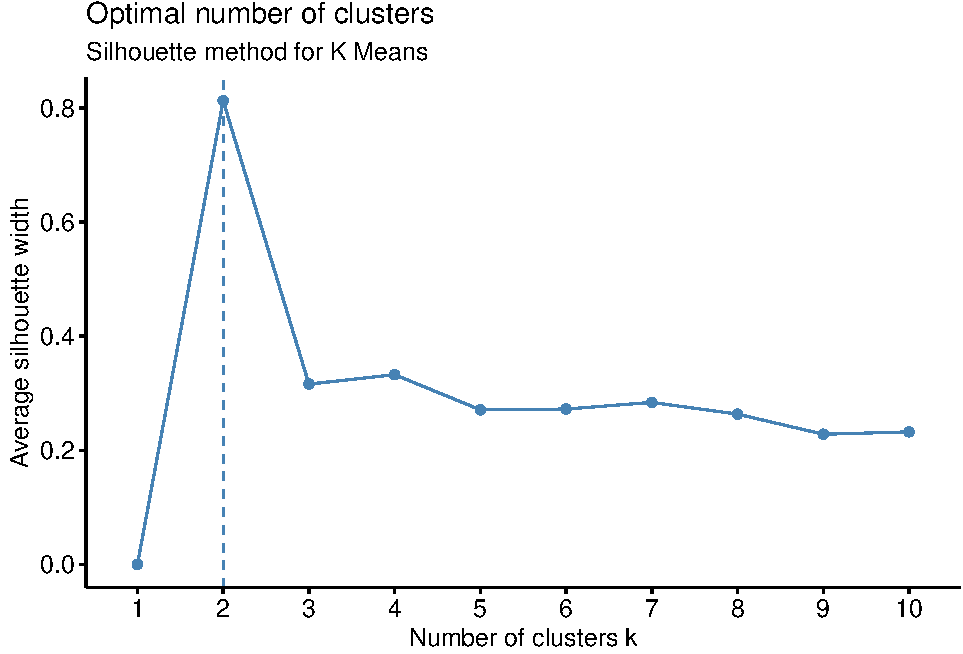
\includegraphics{eda_files/figure-latex/unnamed-chunk-14-1.pdf}

\begin{Shaded}
\begin{Highlighting}[]
\KeywordTok{fviz_nbclust}\NormalTok{(by_country[,}\DecValTok{2}\OperatorTok{:}\KeywordTok{ncol}\NormalTok{(by_country)], kmeans, }\DataTypeTok{nstart =} \DecValTok{25}\NormalTok{,  }\DataTypeTok{method =} \StringTok{"wss"}\NormalTok{, }
             \DataTypeTok{nboot =}\DecValTok{50}\NormalTok{)}\OperatorTok{+}\StringTok{ }\KeywordTok{labs}\NormalTok{(}\DataTypeTok{subtitle =} \StringTok{"Elbow method for K Means"}\NormalTok{)}
\end{Highlighting}
\end{Shaded}

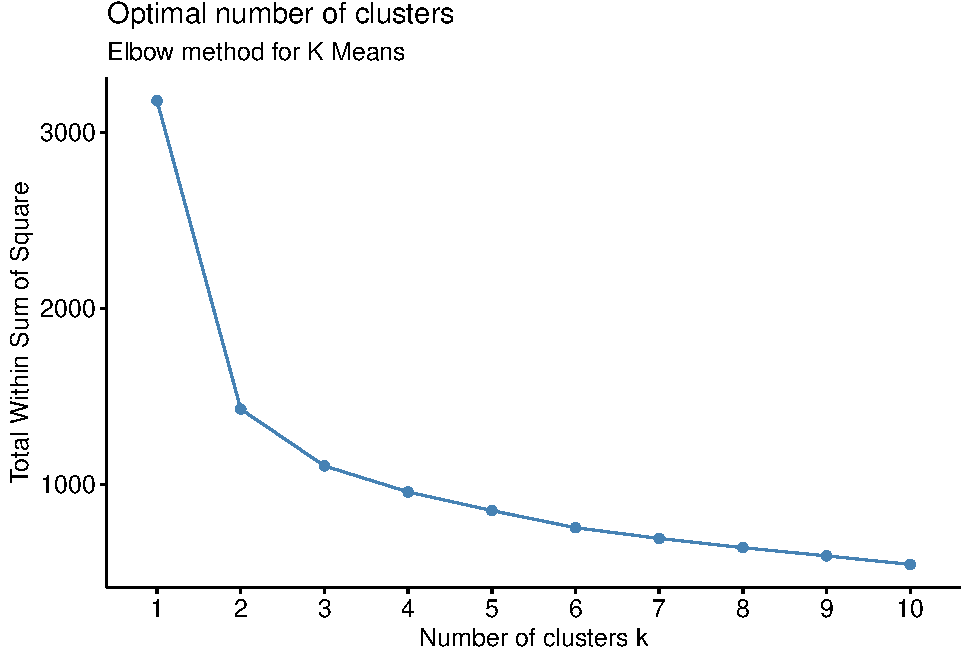
\includegraphics{eda_files/figure-latex/unnamed-chunk-14-2.pdf}

\begin{Shaded}
\begin{Highlighting}[]
\KeywordTok{jpeg}\NormalTok{(}\DataTypeTok{file=}\StringTok{"gap_hac.jpg"}\NormalTok{)}
\KeywordTok{fviz_nbclust}\NormalTok{(by_country[,}\DecValTok{2}\OperatorTok{:}\KeywordTok{ncol}\NormalTok{(by_country)], hcut, }\DataTypeTok{nstart =} \DecValTok{25}\NormalTok{,  }\DataTypeTok{method =} \StringTok{"gap_stat"}\NormalTok{, }
             \DataTypeTok{nboot =} \DecValTok{50}\NormalTok{)}\OperatorTok{+}\KeywordTok{labs}\NormalTok{(}\DataTypeTok{subtitle =} \StringTok{"Gap statistic method for HAC"}\NormalTok{)}
\KeywordTok{dev.off}\NormalTok{()}
\end{Highlighting}
\end{Shaded}

\begin{verbatim}
## pdf 
##   2
\end{verbatim}

\begin{Shaded}
\begin{Highlighting}[]
\KeywordTok{fviz_nbclust}\NormalTok{(by_country[,}\DecValTok{2}\OperatorTok{:}\KeywordTok{ncol}\NormalTok{(by_country)], hcut, }\DataTypeTok{nstart =} \DecValTok{25}\NormalTok{,  }\DataTypeTok{method =} \StringTok{"silhouette"}\NormalTok{, }
             \DataTypeTok{nboot =} \DecValTok{50}\NormalTok{)}\OperatorTok{+}\KeywordTok{labs}\NormalTok{(}\DataTypeTok{subtitle =} \StringTok{"Silhouette method for HAC"}\NormalTok{)}
\end{Highlighting}
\end{Shaded}

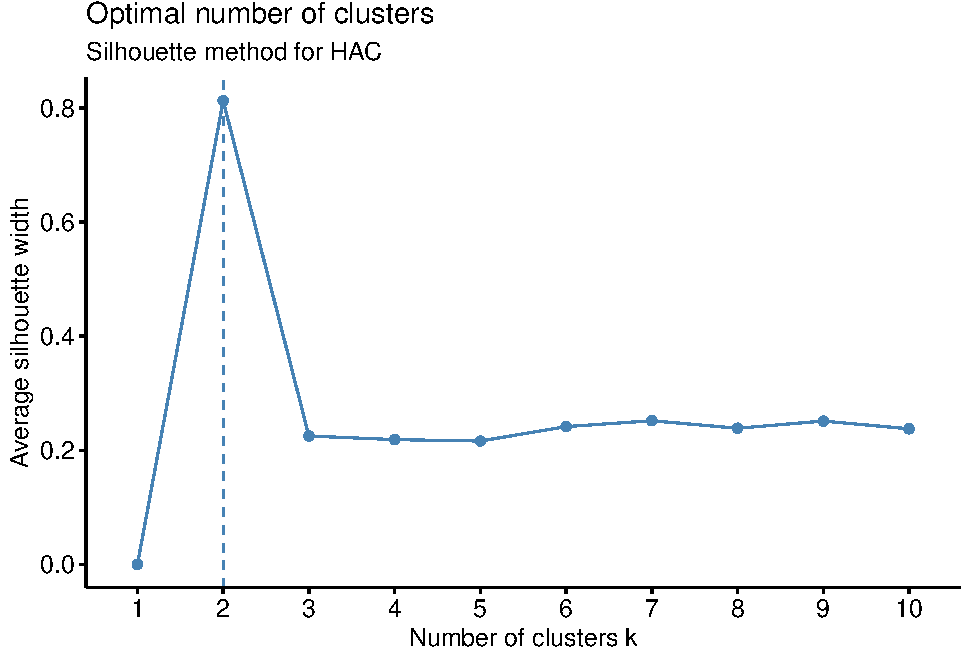
\includegraphics{eda_files/figure-latex/unnamed-chunk-14-3.pdf}

\begin{Shaded}
\begin{Highlighting}[]
\KeywordTok{fviz_nbclust}\NormalTok{(by_country[,}\DecValTok{2}\OperatorTok{:}\KeywordTok{ncol}\NormalTok{(by_country)], hcut, }\DataTypeTok{nstart =} \DecValTok{25}\NormalTok{,  }\DataTypeTok{method =} \StringTok{"wss"}\NormalTok{, }
             \DataTypeTok{nboot =} \DecValTok{50}\NormalTok{)}\OperatorTok{+}\KeywordTok{labs}\NormalTok{(}\DataTypeTok{subtitle =} \StringTok{"Elbow method for HAC"}\NormalTok{)}
\end{Highlighting}
\end{Shaded}

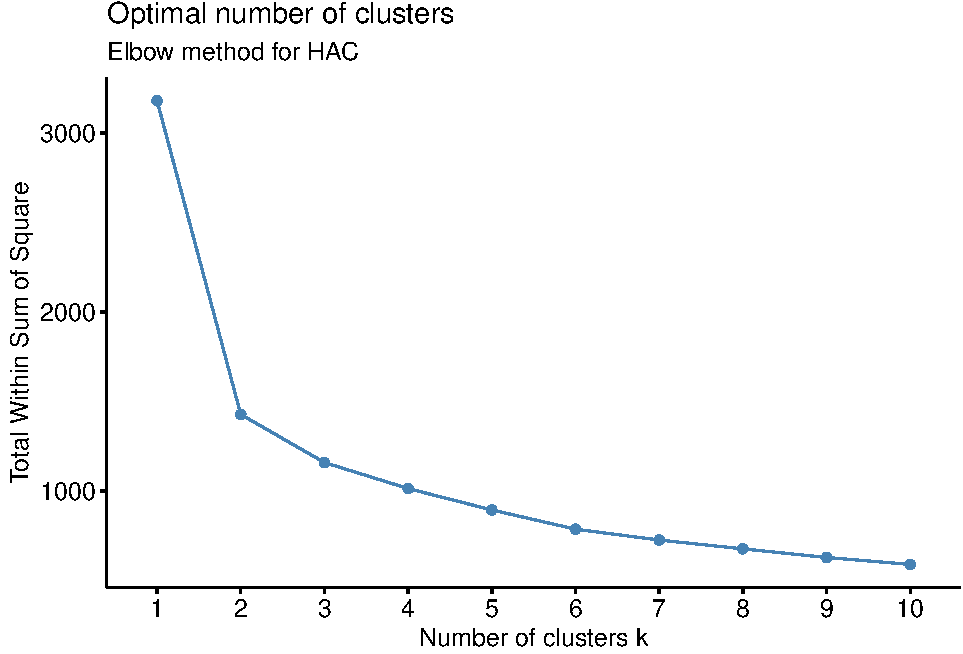
\includegraphics{eda_files/figure-latex/unnamed-chunk-14-4.pdf}

\begin{Shaded}
\begin{Highlighting}[]
\CommentTok{# what to do if the two don't agree?}
\end{Highlighting}
\end{Shaded}

DETERMINING THE LINKAGE CRITERIA:

\begin{Shaded}
\begin{Highlighting}[]
\CommentTok{# Data}
\NormalTok{dist_mat <-}\StringTok{ }\KeywordTok{dist}\NormalTok{(by_country[,}\DecValTok{2}\OperatorTok{:}\KeywordTok{ncol}\NormalTok{(by_country)], }\DataTypeTok{method =} \StringTok{'euclidean'}\NormalTok{)}

\CommentTok{# Hierarchical Agglomerative Clustering}
\NormalTok{h1=}\KeywordTok{hclust}\NormalTok{(dist_mat,}\DataTypeTok{method=}\StringTok{'average'}\NormalTok{)}
\NormalTok{h2=}\KeywordTok{hclust}\NormalTok{(dist_mat,}\DataTypeTok{method=}\StringTok{'complete'}\NormalTok{)}
\NormalTok{h4=}\KeywordTok{hclust}\NormalTok{(dist_mat,}\DataTypeTok{method=}\StringTok{'single'}\NormalTok{)}

\CommentTok{# Cophenetic Distances, for each linkage}
\NormalTok{c1=}\KeywordTok{cophenetic}\NormalTok{(h1)}
\NormalTok{c2=}\KeywordTok{cophenetic}\NormalTok{(h2)}
\NormalTok{c4=}\KeywordTok{cophenetic}\NormalTok{(h4)}

\CommentTok{# Correlations}
\KeywordTok{cor}\NormalTok{(dist_mat,c1) }
\end{Highlighting}
\end{Shaded}

\begin{verbatim}
## [1] 0.9733687
\end{verbatim}

\begin{Shaded}
\begin{Highlighting}[]
\KeywordTok{cor}\NormalTok{(dist_mat,c2) }
\end{Highlighting}
\end{Shaded}

\begin{verbatim}
## [1] 0.8841342
\end{verbatim}

\begin{Shaded}
\begin{Highlighting}[]
\KeywordTok{cor}\NormalTok{(dist_mat,c4)}
\end{Highlighting}
\end{Shaded}

\begin{verbatim}
## [1] 0.9513006
\end{verbatim}

\begin{Shaded}
\begin{Highlighting}[]
\CommentTok{# average is the best linkage method}
\end{Highlighting}
\end{Shaded}

for now, use 3 clusters (for HAC and k-means)

\begin{Shaded}
\begin{Highlighting}[]
\CommentTok{# kmeans clustering}
\KeywordTok{set.seed}\NormalTok{(}\DecValTok{98}\NormalTok{)}
\NormalTok{cluster.results}\FloatTok{.10}\NormalTok{ <-}\StringTok{ }\KeywordTok{kmeans}\NormalTok{(by_country[,}\DecValTok{2}\OperatorTok{:}\KeywordTok{ncol}\NormalTok{(by_country)], }\DecValTok{10}\NormalTok{, }
                          \DataTypeTok{iter.max =} \DecValTok{10}\NormalTok{, }\DataTypeTok{nstart =} \DecValTok{1}\NormalTok{)}

\CommentTok{# cluster.results.6 <- kmeans(by_country[,2:ncol(by_country)], 6, }
\CommentTok{#                           iter.max = 10, nstart = 1)}

\NormalTok{kcluster_by_country =}\StringTok{ }\KeywordTok{data.frame}\NormalTok{(by_country)}
\NormalTok{kcluster_by_country}\OperatorTok{$}\NormalTok{cluster10 <-}\StringTok{ }\KeywordTok{as.factor}\NormalTok{(cluster.results}\FloatTok{.10}\OperatorTok{$}\NormalTok{cluster)}
\CommentTok{# kcluster_by_country$cluster10 <- as.factor(cluster.results.6$cluster)}
\end{Highlighting}
\end{Shaded}

\begin{Shaded}
\begin{Highlighting}[]
\CommentTok{# hierarchical clustering}

\NormalTok{dist_mat <-}\StringTok{ }\KeywordTok{dist}\NormalTok{(by_country[,}\DecValTok{2}\OperatorTok{:}\KeywordTok{ncol}\NormalTok{(by_country)], }\DataTypeTok{method =} \StringTok{'euclidean'}\NormalTok{)}
\NormalTok{hclust_avg <-}\StringTok{ }\KeywordTok{hclust}\NormalTok{(dist_mat, }\DataTypeTok{method =} \StringTok{'average'}\NormalTok{)}

\KeywordTok{jpeg}\NormalTok{(}\DataTypeTok{file=}\StringTok{"cluster_den.jpg"}\NormalTok{)}
\KeywordTok{plot}\NormalTok{(hclust_avg)}
\KeywordTok{dev.off}\NormalTok{()}
\end{Highlighting}
\end{Shaded}

\begin{verbatim}
## pdf 
##   2
\end{verbatim}

\begin{Shaded}
\begin{Highlighting}[]
\NormalTok{cut_avg10 <-}\StringTok{ }\KeywordTok{cutree}\NormalTok{(hclust_avg, }\DataTypeTok{k =} \DecValTok{10}\NormalTok{)}

\NormalTok{avg_dend_obj <-}\StringTok{ }\KeywordTok{as.dendrogram}\NormalTok{(hclust_avg, }\DataTypeTok{h =} \DecValTok{10}\NormalTok{, }\DataTypeTok{leaflab =} \StringTok{"none"}\NormalTok{)}
\KeywordTok{labels}\NormalTok{(avg_dend_obj) <-}\StringTok{ }\KeywordTok{rep}\NormalTok{(}\OtherTok{NA}\NormalTok{, }\KeywordTok{nrow}\NormalTok{(by_country))}
\NormalTok{avg_col_dend10 <-}\StringTok{ }\KeywordTok{color_branches}\NormalTok{(avg_dend_obj, }\DataTypeTok{k =} \DecValTok{10}\NormalTok{)}

\KeywordTok{jpeg}\NormalTok{(}\DataTypeTok{file=}\StringTok{"cluster_den10.jpg"}\NormalTok{)}
\KeywordTok{plot}\NormalTok{(avg_col_dend10)}
\KeywordTok{dev.off}\NormalTok{()}
\end{Highlighting}
\end{Shaded}

\begin{verbatim}
## pdf 
##   2
\end{verbatim}

\begin{Shaded}
\begin{Highlighting}[]
\CommentTok{# jpeg(file="cluster_den6.jpg")}
\CommentTok{# plot(avg_col_dend6)}
\CommentTok{# dev.off()}

\NormalTok{hcluster_by_country10 <-}\StringTok{ }\KeywordTok{mutate}\NormalTok{(by_country, }\DataTypeTok{cluster =}\NormalTok{ cut_avg10)}
\CommentTok{# hcluster_by_country6 <- mutate(by_country, cluster = cut_avg6)}

\NormalTok{hcluster_by_country <-}\StringTok{ }\KeywordTok{data.frame}\NormalTok{(by_country)}

\NormalTok{hcluster_by_country}\OperatorTok{$}\NormalTok{cluster10 <-}\StringTok{ }\KeywordTok{as.factor}\NormalTok{(hcluster_by_country10}\OperatorTok{$}\NormalTok{cluster)}
\CommentTok{# hcluster_by_country$cluster10 <- as.factor(hcluster_by_country6$cluster)}
\end{Highlighting}
\end{Shaded}

\begin{Shaded}
\begin{Highlighting}[]
\CommentTok{# bringing in demographic data; need life expectancy, literacy rate, and fertility rate}
\NormalTok{gdp <-}\StringTok{ }\KeywordTok{read.csv}\NormalTok{(}\StringTok{'data/demographic/gdp.csv'}\NormalTok{)}
\NormalTok{population <-}\StringTok{ }\KeywordTok{read.csv}\NormalTok{(}\StringTok{'data/demographic/population.csv'}\NormalTok{)}
\NormalTok{life_expectancy <-}\StringTok{ }\KeywordTok{read.csv}\NormalTok{(}\StringTok{'data/demographic/life_expectancy.csv'}\NormalTok{)}
\NormalTok{fertility_rate <-}\StringTok{ }\KeywordTok{read.csv}\NormalTok{(}\StringTok{'data/demographic/fertility_rate.csv'}\NormalTok{)}
\NormalTok{literacy_rate <-}\StringTok{ }\KeywordTok{read.csv}\NormalTok{(}\StringTok{'data/demographic/literacy_rate.csv'}\NormalTok{)}
\NormalTok{iso3 <-}\StringTok{ }\KeywordTok{read.csv}\NormalTok{(}\StringTok{'data/demographic/iso3.csv'}\NormalTok{)}
\end{Highlighting}
\end{Shaded}

\begin{Shaded}
\begin{Highlighting}[]
\NormalTok{gdp[gdp}\OperatorTok{$}\NormalTok{Code }\OperatorTok{==}\StringTok{ "ABW"}\NormalTok{, ]}\OperatorTok{$}\NormalTok{GDP =}\StringTok{ }\DecValTok{3202} \OperatorTok{*}\StringTok{ }\DecValTok{10}\OperatorTok{^}\DecValTok{6}
\NormalTok{gdp[gdp}\OperatorTok{$}\NormalTok{Code }\OperatorTok{==}\StringTok{ "AND"}\NormalTok{, ]}\OperatorTok{$}\NormalTok{GDP =}\StringTok{ }\DecValTok{3155} \OperatorTok{*}\StringTok{ }\DecValTok{10}\OperatorTok{^}\DecValTok{6}
\NormalTok{gdp[gdp}\OperatorTok{$}\NormalTok{Code }\OperatorTok{==}\StringTok{ "ERI"}\NormalTok{, ]}\OperatorTok{$}\NormalTok{GDP =}\StringTok{ }\FloatTok{2.07} \OperatorTok{*}\StringTok{ }\DecValTok{10}\OperatorTok{^}\DecValTok{9}
\NormalTok{gdp[gdp}\OperatorTok{$}\NormalTok{Code }\OperatorTok{==}\StringTok{ "GIB"}\NormalTok{, ]}\OperatorTok{$}\NormalTok{GDP =}\StringTok{ }\FloatTok{2885810912.00}
\NormalTok{gdp[gdp}\OperatorTok{$}\NormalTok{Code }\OperatorTok{==}\StringTok{ "GRL"}\NormalTok{, ]}\OperatorTok{$}\NormalTok{GDP =}\StringTok{ }\DecValTok{3052} \OperatorTok{*}\StringTok{ }\DecValTok{10}\OperatorTok{^}\DecValTok{6}
\NormalTok{gdp[gdp}\OperatorTok{$}\NormalTok{Code }\OperatorTok{==}\StringTok{ "LIE"}\NormalTok{, ]}\OperatorTok{$}\NormalTok{GDP =}\StringTok{ }\DecValTok{6839} \OperatorTok{*}\StringTok{ }\DecValTok{10}\OperatorTok{^}\DecValTok{6}
\NormalTok{gdp[gdp}\OperatorTok{$}\NormalTok{Code }\OperatorTok{==}\StringTok{ "MNP"}\NormalTok{, ]}\OperatorTok{$}\NormalTok{GDP =}\StringTok{ }\DecValTok{1182} \OperatorTok{*}\StringTok{ }\DecValTok{10}\OperatorTok{^}\DecValTok{6}
\NormalTok{gdp[gdp}\OperatorTok{$}\NormalTok{Code }\OperatorTok{==}\StringTok{ "NCL"}\NormalTok{, ]}\OperatorTok{$}\NormalTok{GDP =}\StringTok{ }\DecValTok{10} \OperatorTok{*}\StringTok{ }\DecValTok{10}\OperatorTok{^}\DecValTok{9}
\NormalTok{gdp[gdp}\OperatorTok{$}\NormalTok{Code }\OperatorTok{==}\StringTok{ "PYF"}\NormalTok{, ]}\OperatorTok{$}\NormalTok{GDP =}\StringTok{ }\FloatTok{3.45} \OperatorTok{*}\StringTok{ }\DecValTok{10}\OperatorTok{^}\DecValTok{9}
\NormalTok{gdp[gdp}\OperatorTok{$}\NormalTok{Code }\OperatorTok{==}\StringTok{ "SMR"}\NormalTok{, ]}\OperatorTok{$}\NormalTok{GDP =}\StringTok{ }\DecValTok{1616} \OperatorTok{*}\StringTok{ }\DecValTok{10}\OperatorTok{^}\DecValTok{6} 
\NormalTok{gdp[gdp}\OperatorTok{$}\NormalTok{Code }\OperatorTok{==}\StringTok{ "SSD"}\NormalTok{, ]}\OperatorTok{$}\NormalTok{GDP =}\StringTok{ }\FloatTok{1119.7} \OperatorTok{*}\StringTok{ }\DecValTok{10}\OperatorTok{^}\DecValTok{6} 
\NormalTok{gdp[gdp}\OperatorTok{$}\NormalTok{Code }\OperatorTok{==}\StringTok{ "TKM"}\NormalTok{, ]}\OperatorTok{$}\NormalTok{GDP =}\StringTok{ }\DecValTok{45231} \OperatorTok{*}\StringTok{ }\DecValTok{10}\OperatorTok{^}\DecValTok{6} 
\NormalTok{gdp[gdp}\OperatorTok{$}\NormalTok{Code }\OperatorTok{==}\StringTok{ "VEN"}\NormalTok{, ]}\OperatorTok{$}\NormalTok{GDP =}\StringTok{ }\FloatTok{47.26} \OperatorTok{*}\StringTok{ }\DecValTok{10}\OperatorTok{^}\DecValTok{9}
\NormalTok{gdp[gdp}\OperatorTok{$}\NormalTok{Code }\OperatorTok{==}\StringTok{ "YEM"}\NormalTok{, ]}\OperatorTok{$}\NormalTok{GDP =}\StringTok{ }\DecValTok{23486} \OperatorTok{*}\StringTok{ }\DecValTok{10}\OperatorTok{^}\DecValTok{6}
\end{Highlighting}
\end{Shaded}

\begin{Shaded}
\begin{Highlighting}[]
\NormalTok{life_expectancy[life_expectancy}\OperatorTok{$}\NormalTok{Code }\OperatorTok{==}\StringTok{ "AND"}\NormalTok{, ]}\OperatorTok{$}\NormalTok{Expectancy =}\StringTok{ }\FloatTok{84.5}
\NormalTok{life_expectancy[life_expectancy}\OperatorTok{$}\NormalTok{Code }\OperatorTok{==}\StringTok{ "ASM"}\NormalTok{, ]}\OperatorTok{$}\NormalTok{Expectancy =}\StringTok{ }\FloatTok{73.32}
\NormalTok{life_expectancy[life_expectancy}\OperatorTok{$}\NormalTok{Code }\OperatorTok{==}\StringTok{ "CYM"}\NormalTok{, ]}\OperatorTok{$}\NormalTok{Expectancy =}\StringTok{ }\FloatTok{82.19}
\NormalTok{life_expectancy[life_expectancy}\OperatorTok{$}\NormalTok{Code }\OperatorTok{==}\StringTok{ "DMA"}\NormalTok{, ]}\OperatorTok{$}\NormalTok{Expectancy =}\StringTok{ }\FloatTok{76.6}
\NormalTok{life_expectancy[life_expectancy}\OperatorTok{$}\NormalTok{Code }\OperatorTok{==}\StringTok{ "GIB"}\NormalTok{, ]}\OperatorTok{$}\NormalTok{Expectancy =}\StringTok{ }\FloatTok{78.7}
\NormalTok{life_expectancy[life_expectancy}\OperatorTok{$}\NormalTok{Code }\OperatorTok{==}\StringTok{ "KNA"}\NormalTok{, ]}\OperatorTok{$}\NormalTok{Expectancy =}\StringTok{ }\FloatTok{71.34}
\NormalTok{life_expectancy[life_expectancy}\OperatorTok{$}\NormalTok{Code }\OperatorTok{==}\StringTok{ "MCO"}\NormalTok{, ]}\OperatorTok{$}\NormalTok{Expectancy =}\StringTok{ }\FloatTok{89.4}
\NormalTok{life_expectancy[life_expectancy}\OperatorTok{$}\NormalTok{Code }\OperatorTok{==}\StringTok{ "MHL"}\NormalTok{, ]}\OperatorTok{$}\NormalTok{Expectancy =}\StringTok{ }\FloatTok{65.24}
\NormalTok{life_expectancy[life_expectancy}\OperatorTok{$}\NormalTok{Code }\OperatorTok{==}\StringTok{ "MNP"}\NormalTok{, ]}\OperatorTok{$}\NormalTok{Expectancy =}\StringTok{ }\FloatTok{77.1}
\NormalTok{life_expectancy[life_expectancy}\OperatorTok{$}\NormalTok{Code }\OperatorTok{==}\StringTok{ "PLW"}\NormalTok{, ]}\OperatorTok{$}\NormalTok{Expectancy =}\StringTok{ }\FloatTok{69.13}
\NormalTok{life_expectancy[life_expectancy}\OperatorTok{$}\NormalTok{Code }\OperatorTok{==}\StringTok{ "SMR"}\NormalTok{, ]}\OperatorTok{$}\NormalTok{Expectancy =}\StringTok{ }\FloatTok{85.42}
\NormalTok{life_expectancy[life_expectancy}\OperatorTok{$}\NormalTok{Code }\OperatorTok{==}\StringTok{ "TCA"}\NormalTok{, ]}\OperatorTok{$}\NormalTok{Expectancy =}\StringTok{ }\FloatTok{80.6}
\end{Highlighting}
\end{Shaded}

\begin{Shaded}
\begin{Highlighting}[]
\NormalTok{fertility_rate[fertility_rate}\OperatorTok{$}\NormalTok{Code }\OperatorTok{==}\StringTok{ "AND"}\NormalTok{, ]}\OperatorTok{$}\NormalTok{Fertility =}\StringTok{ }\FloatTok{1.3}
\NormalTok{fertility_rate[fertility_rate}\OperatorTok{$}\NormalTok{Code }\OperatorTok{==}\StringTok{ "ASM"}\NormalTok{, ]}\OperatorTok{$}\NormalTok{Fertility =}\StringTok{ }\FloatTok{2.28}
\NormalTok{fertility_rate[fertility_rate}\OperatorTok{$}\NormalTok{Code }\OperatorTok{==}\StringTok{ "CYM"}\NormalTok{, ]}\OperatorTok{$}\NormalTok{Fertility =}\StringTok{ }\FloatTok{1.83}
\NormalTok{fertility_rate[fertility_rate}\OperatorTok{$}\NormalTok{Code }\OperatorTok{==}\StringTok{ "DMA"}\NormalTok{, ]}\OperatorTok{$}\NormalTok{Fertility =}\StringTok{ }\FloatTok{1.9}
\NormalTok{fertility_rate[fertility_rate}\OperatorTok{$}\NormalTok{Code }\OperatorTok{==}\StringTok{ "GIB"}\NormalTok{, ]}\OperatorTok{$}\NormalTok{Fertility =}\StringTok{ }\FloatTok{1.91}
\NormalTok{fertility_rate[fertility_rate}\OperatorTok{$}\NormalTok{Code }\OperatorTok{==}\StringTok{ "KNA"}\NormalTok{, ]}\OperatorTok{$}\NormalTok{Fertility =}\StringTok{ }\FloatTok{2.1}
\NormalTok{fertility_rate[fertility_rate}\OperatorTok{$}\NormalTok{Code }\OperatorTok{==}\StringTok{ "MCO"}\NormalTok{, ]}\OperatorTok{$}\NormalTok{Fertility =}\StringTok{ }\FloatTok{1.52}
\NormalTok{fertility_rate[fertility_rate}\OperatorTok{$}\NormalTok{Code }\OperatorTok{==}\StringTok{ "MHL"}\NormalTok{, ]}\OperatorTok{$}\NormalTok{Fertility =}\StringTok{ }\FloatTok{4.5}
\NormalTok{fertility_rate[fertility_rate}\OperatorTok{$}\NormalTok{Code }\OperatorTok{==}\StringTok{ "MNP"}\NormalTok{, ]}\OperatorTok{$}\NormalTok{Fertility =}\StringTok{ }\FloatTok{2.66}
\NormalTok{fertility_rate[fertility_rate}\OperatorTok{$}\NormalTok{Code }\OperatorTok{==}\StringTok{ "PLW"}\NormalTok{, ]}\OperatorTok{$}\NormalTok{Fertility =}\StringTok{ }\FloatTok{2.21}
\NormalTok{fertility_rate[fertility_rate}\OperatorTok{$}\NormalTok{Code }\OperatorTok{==}\StringTok{ "SMR"}\NormalTok{, ]}\OperatorTok{$}\NormalTok{Fertility =}\StringTok{ }\FloatTok{1.3}
\NormalTok{fertility_rate[fertility_rate}\OperatorTok{$}\NormalTok{Code }\OperatorTok{==}\StringTok{ "TCA"}\NormalTok{, ]}\OperatorTok{$}\NormalTok{Fertility =}\StringTok{ }\FloatTok{1.7}
\end{Highlighting}
\end{Shaded}

\begin{Shaded}
\begin{Highlighting}[]
\CommentTok{# some data cleaning on literacy rate -- need to note how not all of them were pulled from}
\CommentTok{# 2020}
\NormalTok{literacy_rate <-}\StringTok{ }\KeywordTok{merge}\NormalTok{(literacy_rate, iso3, }\DataTypeTok{by.x =} \StringTok{"country"}\NormalTok{, }\DataTypeTok{by.y =} \StringTok{"Country"}\NormalTok{)}
\NormalTok{literacy_rate <-}\StringTok{ }\KeywordTok{subset}\NormalTok{(literacy_rate, }\DataTypeTok{select =} \KeywordTok{c}\NormalTok{(latestRate, Alpha.}\FloatTok{3.}\NormalTok{code))}
\KeywordTok{colnames}\NormalTok{(literacy_rate) <-}\StringTok{ }\KeywordTok{c}\NormalTok{(}\StringTok{'literacy'}\NormalTok{, }\StringTok{'Code'}\NormalTok{)}
\NormalTok{literacy_rate}\OperatorTok{$}\NormalTok{Code <-}\StringTok{ }\KeywordTok{trimws}\NormalTok{(literacy_rate}\OperatorTok{$}\NormalTok{Code)}
\end{Highlighting}
\end{Shaded}

\begin{Shaded}
\begin{Highlighting}[]
\NormalTok{master_df_k <-}\StringTok{ }\KeywordTok{merge}\NormalTok{(kcluster_by_country, gdp, }\DataTypeTok{by.x =} \StringTok{"ISO3"}\NormalTok{, }\DataTypeTok{by.y =} \StringTok{"Code"}\NormalTok{)}
\NormalTok{master_df_k <-}\StringTok{ }\KeywordTok{merge}\NormalTok{(master_df_k, population, }\DataTypeTok{by.x =} \StringTok{"ISO3"}\NormalTok{, }\DataTypeTok{by.y =} \StringTok{"Code"}\NormalTok{)}
\NormalTok{master_df_k <-}\StringTok{ }\KeywordTok{merge}\NormalTok{(master_df_k, life_expectancy, }\DataTypeTok{by.x =} \StringTok{"ISO3"}\NormalTok{, }\DataTypeTok{by.y =} \StringTok{"Code"}\NormalTok{)}
\NormalTok{master_df_k <-}\StringTok{ }\KeywordTok{merge}\NormalTok{(master_df_k, fertility_rate, }\DataTypeTok{by.x =} \StringTok{"ISO3"}\NormalTok{, }\DataTypeTok{by.y =} \StringTok{"Code"}\NormalTok{)}
\NormalTok{master_df_k <-}\StringTok{ }\KeywordTok{merge}\NormalTok{(master_df_k, literacy_rate, }\DataTypeTok{by.x =} \StringTok{"ISO3"}\NormalTok{, }\DataTypeTok{by.y =} \StringTok{"Code"}\NormalTok{)}
\NormalTok{master_df_k <-}\StringTok{ }\KeywordTok{subset}\NormalTok{(master_df_k, }\DataTypeTok{select =} \OperatorTok{-}\KeywordTok{c}\NormalTok{(Name.x, X.x, Name.y, X.y))}

\NormalTok{master_df_h <-}\StringTok{ }\KeywordTok{merge}\NormalTok{(hcluster_by_country, gdp, }\DataTypeTok{by.x =} \StringTok{"ISO3"}\NormalTok{, }\DataTypeTok{by.y =} \StringTok{"Code"}\NormalTok{)}
\NormalTok{master_df_h <-}\StringTok{ }\KeywordTok{merge}\NormalTok{(master_df_h, population, }\DataTypeTok{by.x =} \StringTok{"ISO3"}\NormalTok{, }\DataTypeTok{by.y =} \StringTok{"Code"}\NormalTok{)}
\NormalTok{master_df_h <-}\StringTok{ }\KeywordTok{merge}\NormalTok{(master_df_h, life_expectancy, }\DataTypeTok{by.x =} \StringTok{"ISO3"}\NormalTok{, }\DataTypeTok{by.y =} \StringTok{"Code"}\NormalTok{)}
\NormalTok{master_df_h <-}\StringTok{ }\KeywordTok{merge}\NormalTok{(master_df_h, fertility_rate, }\DataTypeTok{by.x =} \StringTok{"ISO3"}\NormalTok{, }\DataTypeTok{by.y =} \StringTok{"Code"}\NormalTok{)}
\NormalTok{master_df_h <-}\StringTok{ }\KeywordTok{merge}\NormalTok{(master_df_h, literacy_rate, }\DataTypeTok{by.x =} \StringTok{"ISO3"}\NormalTok{, }\DataTypeTok{by.y =} \StringTok{"Code"}\NormalTok{)}
\NormalTok{master_df_h <-}\StringTok{ }\KeywordTok{subset}\NormalTok{(master_df_h, }\DataTypeTok{select =} \OperatorTok{-}\KeywordTok{c}\NormalTok{(Name.x, X.x, Name.y, X.y))}
\end{Highlighting}
\end{Shaded}

\begin{Shaded}
\begin{Highlighting}[]
\CommentTok{# anova stuff}
\CommentTok{# histograms or boxplots -- distribution of these variables across these clusters change}
\CommentTok{# for ones that are significant -- look for outliers!}

\NormalTok{k_gdp <-}\StringTok{ }\KeywordTok{aov}\NormalTok{(GDP }\OperatorTok{~}\StringTok{ }\NormalTok{cluster10, }\DataTypeTok{data =}\NormalTok{ master_df_k)}
\NormalTok{k_pop <-}\StringTok{ }\KeywordTok{aov}\NormalTok{(Pop }\OperatorTok{~}\StringTok{ }\NormalTok{cluster10, }\DataTypeTok{data =}\NormalTok{ master_df_k) }
\NormalTok{k_exp <-}\StringTok{ }\KeywordTok{aov}\NormalTok{(Expectancy }\OperatorTok{~}\StringTok{ }\NormalTok{cluster10, }\DataTypeTok{data =}\NormalTok{ master_df_k) }
\NormalTok{k_fert <-}\StringTok{ }\KeywordTok{aov}\NormalTok{(Fertility }\OperatorTok{~}\StringTok{ }\NormalTok{cluster10, }\DataTypeTok{data =}\NormalTok{ master_df_k) }
\NormalTok{k_lit <-}\StringTok{ }\KeywordTok{aov}\NormalTok{(literacy }\OperatorTok{~}\StringTok{ }\NormalTok{cluster10, }\DataTypeTok{data =}\NormalTok{ master_df_k) }

\KeywordTok{summary}\NormalTok{(k_gdp)}
\end{Highlighting}
\end{Shaded}

\begin{verbatim}
##              Df    Sum Sq   Mean Sq F value Pr(>F)
## cluster10     9 4.984e+25 5.538e+24   1.509  0.148
## Residuals   179 6.569e+26 3.670e+24
\end{verbatim}

\begin{Shaded}
\begin{Highlighting}[]
\KeywordTok{summary}\NormalTok{(k_pop)}
\end{Highlighting}
\end{Shaded}

\begin{verbatim}
##              Df    Sum Sq   Mean Sq F value Pr(>F)
## cluster10     9 2.762e+17 3.069e+16   1.423  0.181
## Residuals   179 3.861e+18 2.157e+16
\end{verbatim}

\begin{Shaded}
\begin{Highlighting}[]
\KeywordTok{summary}\NormalTok{(k_exp)}
\end{Highlighting}
\end{Shaded}

\begin{verbatim}
##              Df Sum Sq Mean Sq F value  Pr(>F)    
## cluster10     9   2221  246.79   5.405 1.5e-06 ***
## Residuals   179   8174   45.66                    
## ---
## Signif. codes:  0 '***' 0.001 '**' 0.01 '*' 0.05 '.' 0.1 ' ' 1
\end{verbatim}

\begin{Shaded}
\begin{Highlighting}[]
\KeywordTok{summary}\NormalTok{(k_fert)}
\end{Highlighting}
\end{Shaded}

\begin{verbatim}
##              Df Sum Sq Mean Sq F value   Pr(>F)    
## cluster10     9  40.66   4.517   3.429 0.000644 ***
## Residuals   179 235.84   1.318                     
## ---
## Signif. codes:  0 '***' 0.001 '**' 0.01 '*' 0.05 '.' 0.1 ' ' 1
\end{verbatim}

\begin{Shaded}
\begin{Highlighting}[]
\KeywordTok{summary}\NormalTok{(k_lit)}
\end{Highlighting}
\end{Shaded}

\begin{verbatim}
##              Df Sum Sq Mean Sq F value  Pr(>F)   
## cluster10     9   8491   943.4    3.11 0.00169 **
## Residuals   179  54299   303.3                   
## ---
## Signif. codes:  0 '***' 0.001 '**' 0.01 '*' 0.05 '.' 0.1 ' ' 1
\end{verbatim}

\begin{Shaded}
\begin{Highlighting}[]
\NormalTok{h_gdp <-}\StringTok{ }\KeywordTok{aov}\NormalTok{(GDP }\OperatorTok{~}\StringTok{ }\NormalTok{cluster10, }\DataTypeTok{data =}\NormalTok{ master_df_h)}
\NormalTok{h_pop <-}\StringTok{ }\KeywordTok{aov}\NormalTok{(Pop }\OperatorTok{~}\StringTok{ }\NormalTok{cluster10, }\DataTypeTok{data =}\NormalTok{ master_df_h) }
\NormalTok{h_exp <-}\StringTok{ }\KeywordTok{aov}\NormalTok{(Expectancy }\OperatorTok{~}\StringTok{ }\NormalTok{cluster10, }\DataTypeTok{data =}\NormalTok{ master_df_h) }
\NormalTok{h_fert <-}\StringTok{ }\KeywordTok{aov}\NormalTok{(Fertility }\OperatorTok{~}\StringTok{ }\NormalTok{cluster10, }\DataTypeTok{data =}\NormalTok{ master_df_h) }
\NormalTok{h_lit <-}\StringTok{ }\KeywordTok{aov}\NormalTok{(literacy }\OperatorTok{~}\StringTok{ }\NormalTok{cluster10, }\DataTypeTok{data =}\NormalTok{ master_df_h) }

\KeywordTok{summary}\NormalTok{(h_gdp)}
\end{Highlighting}
\end{Shaded}

\begin{verbatim}
##              Df    Sum Sq   Mean Sq F value   Pr(>F)    
## cluster10     8 1.104e+26 1.380e+25   4.166 0.000136 ***
## Residuals   180 5.964e+26 3.313e+24                     
## ---
## Signif. codes:  0 '***' 0.001 '**' 0.01 '*' 0.05 '.' 0.1 ' ' 1
\end{verbatim}

\begin{Shaded}
\begin{Highlighting}[]
\KeywordTok{summary}\NormalTok{(h_pop)}
\end{Highlighting}
\end{Shaded}

\begin{verbatim}
##              Df    Sum Sq   Mean Sq F value Pr(>F)
## cluster10     8 3.348e+16 4.184e+15   0.184  0.993
## Residuals   180 4.104e+18 2.280e+16
\end{verbatim}

\begin{Shaded}
\begin{Highlighting}[]
\KeywordTok{summary}\NormalTok{(h_exp)}
\end{Highlighting}
\end{Shaded}

\begin{verbatim}
##              Df Sum Sq Mean Sq F value  Pr(>F)   
## cluster10     8   1146  143.24   2.788 0.00623 **
## Residuals   180   9249   51.38                   
## ---
## Signif. codes:  0 '***' 0.001 '**' 0.01 '*' 0.05 '.' 0.1 ' ' 1
\end{verbatim}

\begin{Shaded}
\begin{Highlighting}[]
\KeywordTok{summary}\NormalTok{(h_fert)}
\end{Highlighting}
\end{Shaded}

\begin{verbatim}
##              Df Sum Sq Mean Sq F value Pr(>F)
## cluster10     8  18.05   2.256   1.571  0.136
## Residuals   180 258.44   1.436
\end{verbatim}

\begin{Shaded}
\begin{Highlighting}[]
\KeywordTok{summary}\NormalTok{(h_lit)}
\end{Highlighting}
\end{Shaded}

\begin{verbatim}
##              Df Sum Sq Mean Sq F value Pr(>F)
## cluster10     8   3473   434.2   1.318  0.237
## Residuals   180  59317   329.5
\end{verbatim}

\url{https://gist.github.com/tadast/8827699}
\url{https://worldpopulationreview.com/country-rankings/literacy-rate-by-country}
\url{https://www.datanovia.com/en/lessons/determining-the-optimal-number-of-clusters-3-must-know-methods/}

\begin{Shaded}
\begin{Highlighting}[]
\CommentTok{# need to merge continent and development level into the data}
\NormalTok{continents <-}\StringTok{ }\KeywordTok{read.csv}\NormalTok{(}\StringTok{'data/demographic/continent.csv'}\NormalTok{)}
\NormalTok{continents <-}\StringTok{ }\KeywordTok{subset}\NormalTok{(continents, }\DataTypeTok{select =} \KeywordTok{c}\NormalTok{(continent, code_}\DecValTok{3}\NormalTok{))}
\NormalTok{old <-}\StringTok{ }\KeywordTok{c}\NormalTok{(}\StringTok{"Asia"}\NormalTok{, }\StringTok{"Europe"}\NormalTok{, }\StringTok{"Africa"}\NormalTok{, }\StringTok{"Oceania"}\NormalTok{, }\StringTok{"Americas"}\NormalTok{)}
\NormalTok{new <-}\StringTok{ }\DecValTok{1}\OperatorTok{:}\KeywordTok{length}\NormalTok{(old)}
\NormalTok{continents}\OperatorTok{$}\NormalTok{continent[continents}\OperatorTok{$}\NormalTok{continent }\OperatorTok\StringTok{ }\NormalTok{old] <-}\StringTok{ }\NormalTok{new[}\KeywordTok{match}\NormalTok{(continents}\OperatorTok{$}\NormalTok{continent, }
\NormalTok{                                                                 old, }\DataTypeTok{nomatch =} \DecValTok{0}\NormalTok{)]}
\NormalTok{continents}\OperatorTok{$}\NormalTok{continent <-}\StringTok{ }\KeywordTok{as.numeric}\NormalTok{(continents}\OperatorTok{$}\NormalTok{continent)}
\NormalTok{master_df_k_continent <-}\StringTok{ }\KeywordTok{merge}\NormalTok{(master_df_k, continents, }\DataTypeTok{by.x =} \StringTok{"ISO3"}\NormalTok{, }\DataTypeTok{by.y =} \StringTok{"code_3"}\NormalTok{)}
\NormalTok{master_df_h_continent <-}\StringTok{ }\KeywordTok{merge}\NormalTok{(master_df_h, continents, }\DataTypeTok{by.x =} \StringTok{"ISO3"}\NormalTok{, }\DataTypeTok{by.y =} \StringTok{"code_3"}\NormalTok{)}
\end{Highlighting}
\end{Shaded}

HDI classifications are based on HDI fixed cutoff points, which are
derived from the quartiles of dis- tributions of the component
indicators. The cutoff-points are HDI of less than 0.550 for low human
development, 0.550--0.699 for medium human development, 0.700--0.799 for
high human development and 0.800 or greater for very high human
development.

\url{https://hdr.undp.org/en/content/human-development-report-2020-readers-guide}

\begin{Shaded}
\begin{Highlighting}[]
\NormalTok{hdi <-}\StringTok{ }\KeywordTok{read.csv}\NormalTok{(}\StringTok{'data/demographic/hdi.csv'}\NormalTok{)}
\NormalTok{hdi <-}\StringTok{ }\KeywordTok{merge}\NormalTok{(hdi, iso3, }\DataTypeTok{by.x =} \StringTok{"country"}\NormalTok{, }\DataTypeTok{by.y =} \StringTok{"Country"}\NormalTok{)}
\NormalTok{hdi <-}\StringTok{ }\KeywordTok{subset}\NormalTok{(hdi, }\DataTypeTok{select =} \KeywordTok{c}\NormalTok{(hdi, Alpha.}\FloatTok{3.}\NormalTok{code))}
\KeywordTok{colnames}\NormalTok{(hdi) <-}\StringTok{ }\KeywordTok{c}\NormalTok{(}\StringTok{'hdi'}\NormalTok{, }\StringTok{'Code'}\NormalTok{)}
\NormalTok{hdi}\OperatorTok{$}\NormalTok{development <-}\StringTok{ }\KeywordTok{rep}\NormalTok{(}\DecValTok{1}\NormalTok{, }\KeywordTok{nrow}\NormalTok{(hdi))}
\NormalTok{hdi[hdi}\OperatorTok{$}\NormalTok{hdi }\OperatorTok{>=}\StringTok{ }\FloatTok{0.55} \OperatorTok{&}\StringTok{ }\NormalTok{hdi}\OperatorTok{$}\NormalTok{hdi }\OperatorTok{<=}\StringTok{ }\FloatTok{0.699}\NormalTok{, ]}\OperatorTok{$}\NormalTok{development <-}\StringTok{ }\DecValTok{2}
\NormalTok{hdi[hdi}\OperatorTok{$}\NormalTok{hdi }\OperatorTok{>=}\StringTok{ }\FloatTok{0.7} \OperatorTok{&}\StringTok{ }\NormalTok{hdi}\OperatorTok{$}\NormalTok{hdi }\OperatorTok{<=}\StringTok{ }\FloatTok{0.799}\NormalTok{, ]}\OperatorTok{$}\NormalTok{development <-}\StringTok{ }\DecValTok{3}
\NormalTok{hdi[hdi}\OperatorTok{$}\NormalTok{hdi }\OperatorTok{>=}\StringTok{ }\FloatTok{0.8}\NormalTok{, ]}\OperatorTok{$}\NormalTok{development <-}\StringTok{ }\DecValTok{4}
\NormalTok{hdi}\OperatorTok{$}\NormalTok{Code <-}\StringTok{ }\KeywordTok{trimws}\NormalTok{(hdi}\OperatorTok{$}\NormalTok{Code)}

\NormalTok{master_df_k_hdi <-}\StringTok{ }\KeywordTok{merge}\NormalTok{(master_df_k, hdi, }\DataTypeTok{by.x =} \StringTok{"ISO3"}\NormalTok{, }\DataTypeTok{by.y =} \StringTok{"Code"}\NormalTok{)}
\NormalTok{master_df_h_hdi <-}\StringTok{ }\KeywordTok{merge}\NormalTok{(master_df_h, hdi, }\DataTypeTok{by.x =} \StringTok{"ISO3"}\NormalTok{, }\DataTypeTok{by.y =} \StringTok{"Code"}\NormalTok{)}
\end{Highlighting}
\end{Shaded}

\begin{Shaded}
\begin{Highlighting}[]
\KeywordTok{rand.index}\NormalTok{(}\KeywordTok{as.numeric}\NormalTok{(}\KeywordTok{levels}\NormalTok{(master_df_k_continent}\OperatorTok{$}\NormalTok{cluster10))[master_df_k_continent}\OperatorTok{$}\NormalTok{cluster10],}
\NormalTok{           master_df_k_continent}\OperatorTok{$}\NormalTok{continent)}
\end{Highlighting}
\end{Shaded}

\begin{verbatim}
## [1] 0.6787684
\end{verbatim}

\begin{Shaded}
\begin{Highlighting}[]
\KeywordTok{rand.index}\NormalTok{(}\KeywordTok{as.numeric}\NormalTok{(}\KeywordTok{levels}\NormalTok{(master_df_h_continent}\OperatorTok{$}\NormalTok{cluster10))[master_df_h_continent}\OperatorTok{$}\NormalTok{cluster10],}
\NormalTok{           master_df_k_continent}\OperatorTok{$}\NormalTok{continent)}
\end{Highlighting}
\end{Shaded}

\begin{verbatim}
## [1] 0.3761117
\end{verbatim}

\begin{Shaded}
\begin{Highlighting}[]
\KeywordTok{rand.index}\NormalTok{(}\KeywordTok{as.numeric}\NormalTok{(}\KeywordTok{levels}\NormalTok{(master_df_h_continent}\OperatorTok{$}\NormalTok{cluster10))[master_df_h_continent}\OperatorTok{$}\NormalTok{cluster10],}
           \KeywordTok{as.numeric}\NormalTok{(}\KeywordTok{levels}\NormalTok{(master_df_k_continent}\OperatorTok{$}\NormalTok{cluster10))[master_df_k_continent}\OperatorTok{$}\NormalTok{cluster10])}
\end{Highlighting}
\end{Shaded}

\begin{verbatim}
## [1] 0.4467522
\end{verbatim}

\begin{Shaded}
\begin{Highlighting}[]
\KeywordTok{rand.index}\NormalTok{(}\KeywordTok{as.numeric}\NormalTok{(}\KeywordTok{levels}\NormalTok{(master_df_k_hdi}\OperatorTok{$}\NormalTok{cluster10))[master_df_k_hdi}\OperatorTok{$}\NormalTok{cluster10], }
\NormalTok{           master_df_k_hdi}\OperatorTok{$}\NormalTok{development)}
\end{Highlighting}
\end{Shaded}

\begin{verbatim}
## [1] 0.6513932
\end{verbatim}

\begin{Shaded}
\begin{Highlighting}[]
\KeywordTok{rand.index}\NormalTok{(}\KeywordTok{as.numeric}\NormalTok{(}\KeywordTok{levels}\NormalTok{(master_df_h_hdi}\OperatorTok{$}\NormalTok{cluster10))[master_df_h_hdi}\OperatorTok{$}\NormalTok{cluster10], }
\NormalTok{           master_df_h_hdi}\OperatorTok{$}\NormalTok{development)}
\end{Highlighting}
\end{Shaded}

\begin{verbatim}
## [1] 0.3738562
\end{verbatim}

\begin{Shaded}
\begin{Highlighting}[]
\CommentTok{# trying to explain these results? need similar data for developed vs undeveloped}
\CommentTok{# be prepared to justify why!!}
\end{Highlighting}
\end{Shaded}

\begin{Shaded}
\begin{Highlighting}[]
\CommentTok{# generating graphs: possible pairs}

\CommentTok{#       [,1]         [,2]        }
\CommentTok{#  [1,] "GDP"        "Pop"       }
\CommentTok{#  [2,] "GDP"        "Expectancy"}
\CommentTok{#  [3,] "GDP"        "Fertility" }
\CommentTok{#  [4,] "GDP"        "literacy"  }
\CommentTok{#  [5,] "Pop"        "Expectancy"}
\CommentTok{#  [6,] "Pop"        "Fertility" }
\CommentTok{#  [7,] "Pop"        "literacy"  }
\CommentTok{#  [8,] "Expectancy" "Fertility" }
\CommentTok{#  [9,] "Expectancy" "literacy"  }
\CommentTok{# [10,] "Fertility"  "literacy"  }

\NormalTok{vars <-}\StringTok{ }\KeywordTok{c}\NormalTok{(}\StringTok{"GDP"}\NormalTok{, }\StringTok{"Pop"}\NormalTok{, }\StringTok{"Expectancy"}\NormalTok{, }\StringTok{"Fertility"}\NormalTok{, }\StringTok{"literacy"}\NormalTok{)}
\NormalTok{pairs <-}\StringTok{ }\KeywordTok{t}\NormalTok{(}\KeywordTok{combn}\NormalTok{(vars, }\DecValTok{2}\NormalTok{))}

\NormalTok{p2 <-}\StringTok{ }\KeywordTok{ggplot}\NormalTok{(master_df_k, }\KeywordTok{aes}\NormalTok{(}\DataTypeTok{x =} \KeywordTok{log}\NormalTok{(GDP), }\DataTypeTok{y =} \KeywordTok{log}\NormalTok{(Pop), }\DataTypeTok{color =}\NormalTok{ cluster10)) }\OperatorTok{+}
\StringTok{  }\KeywordTok{geom_point}\NormalTok{(}\DataTypeTok{size=}\DecValTok{2}\NormalTok{)}
\NormalTok{p2 }\OperatorTok{+}\StringTok{ }\KeywordTok{ggtitle}\NormalTok{(}\StringTok{"K-Means: 10 Clusters"}\NormalTok{) }\OperatorTok{+}\StringTok{ }\KeywordTok{scale_fill_brewer}\NormalTok{(}\DataTypeTok{palette=}\StringTok{"Set3"}\NormalTok{)}
\end{Highlighting}
\end{Shaded}

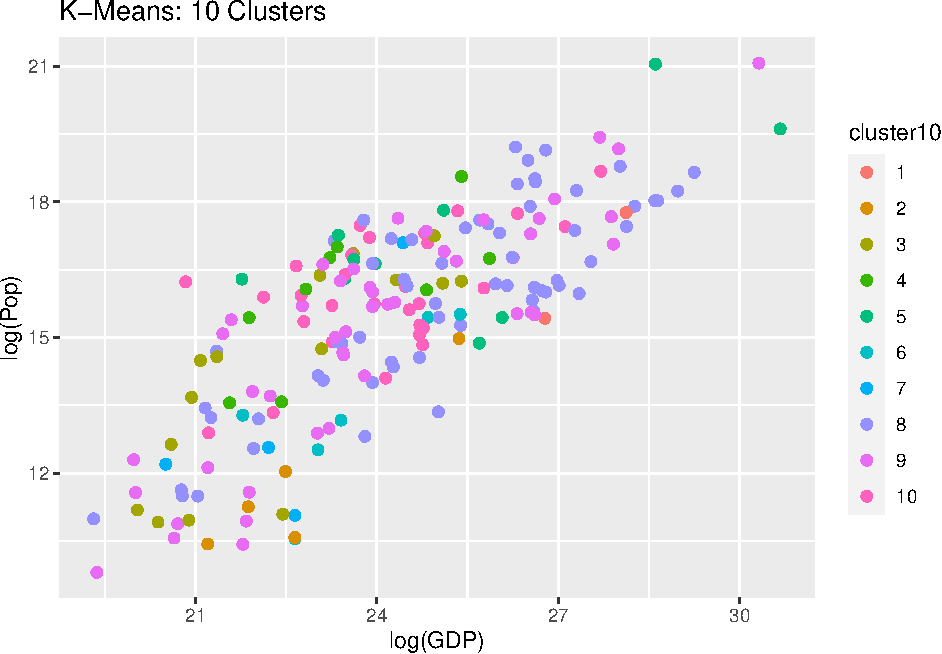
\includegraphics{eda_files/figure-latex/unnamed-chunk-29-1.pdf}

\begin{Shaded}
\begin{Highlighting}[]
\NormalTok{p2 <-}\StringTok{ }\KeywordTok{ggplot}\NormalTok{(master_df_k, }\KeywordTok{aes}\NormalTok{(}\DataTypeTok{x =} \KeywordTok{log}\NormalTok{(GDP), }\DataTypeTok{y =} \KeywordTok{log}\NormalTok{(Expectancy), }\DataTypeTok{color =}\NormalTok{ cluster10)) }\OperatorTok{+}
\StringTok{  }\KeywordTok{geom_point}\NormalTok{(}\DataTypeTok{size=}\DecValTok{2}\NormalTok{)}
\NormalTok{p2 }\OperatorTok{+}\StringTok{ }\KeywordTok{ggtitle}\NormalTok{(}\StringTok{"K-Means: 10 Clusters"}\NormalTok{) }\OperatorTok{+}\StringTok{ }\KeywordTok{scale_fill_brewer}\NormalTok{(}\DataTypeTok{palette=}\StringTok{"Set3"}\NormalTok{)}
\end{Highlighting}
\end{Shaded}

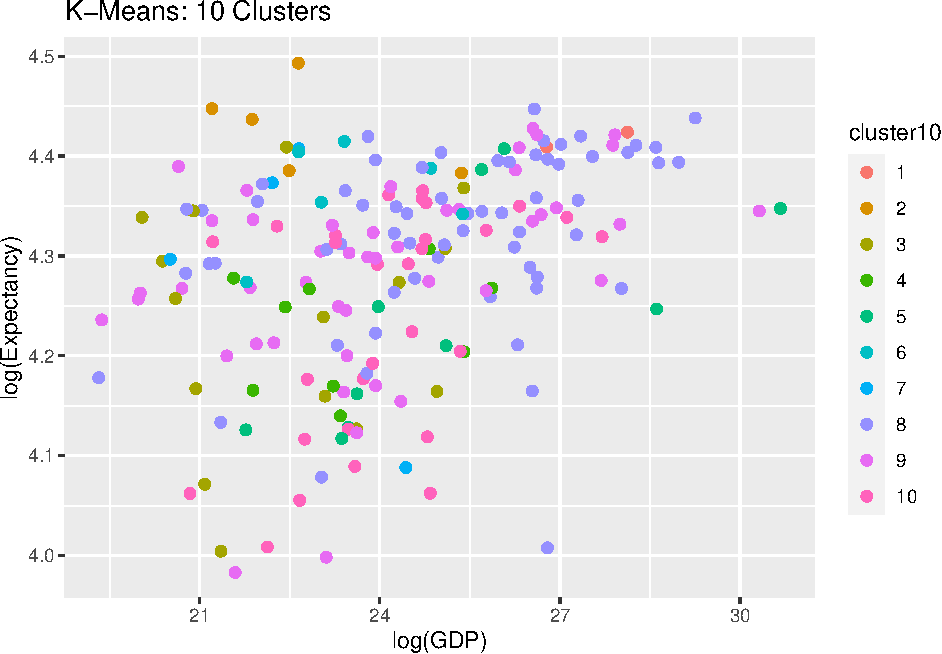
\includegraphics{eda_files/figure-latex/unnamed-chunk-29-2.pdf}

\begin{Shaded}
\begin{Highlighting}[]
\NormalTok{p2 <-}\StringTok{ }\KeywordTok{ggplot}\NormalTok{(master_df_k, }\KeywordTok{aes}\NormalTok{(}\DataTypeTok{x =} \KeywordTok{log}\NormalTok{(GDP), }\DataTypeTok{y =} \KeywordTok{log}\NormalTok{(Fertility), }\DataTypeTok{color =}\NormalTok{ cluster10)) }\OperatorTok{+}
\StringTok{  }\KeywordTok{geom_point}\NormalTok{(}\DataTypeTok{size=}\DecValTok{2}\NormalTok{)}
\NormalTok{p2 }\OperatorTok{+}\StringTok{ }\KeywordTok{ggtitle}\NormalTok{(}\StringTok{"K-Means: 10 Clusters"}\NormalTok{) }\OperatorTok{+}\StringTok{ }\KeywordTok{scale_fill_brewer}\NormalTok{(}\DataTypeTok{palette=}\StringTok{"Set3"}\NormalTok{)}
\end{Highlighting}
\end{Shaded}

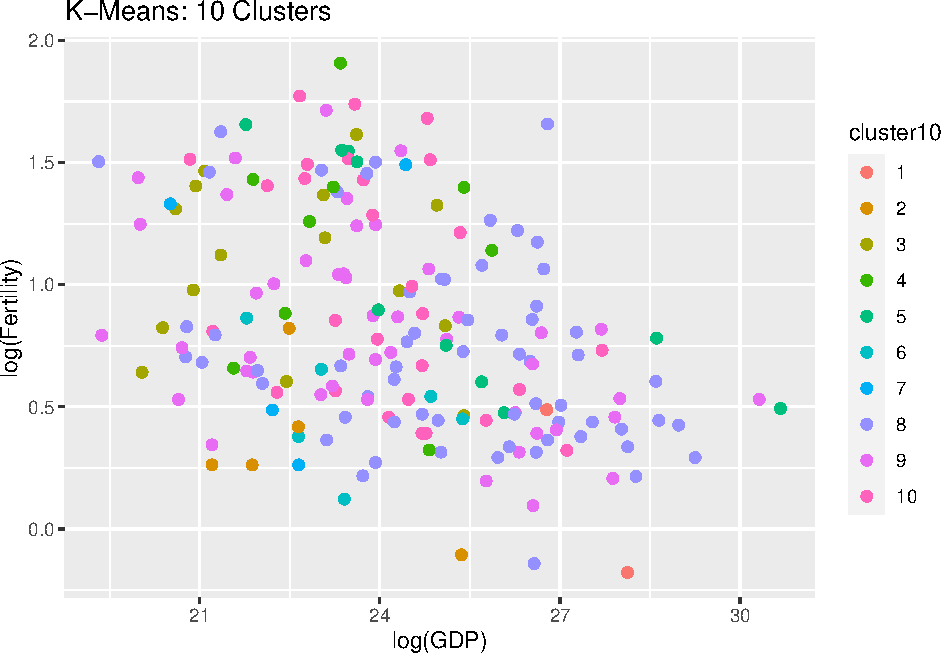
\includegraphics{eda_files/figure-latex/unnamed-chunk-29-3.pdf}

\begin{Shaded}
\begin{Highlighting}[]
\NormalTok{p2 <-}\StringTok{ }\KeywordTok{ggplot}\NormalTok{(master_df_k, }\KeywordTok{aes}\NormalTok{(}\DataTypeTok{x =} \KeywordTok{log}\NormalTok{(GDP), }\DataTypeTok{y =} \KeywordTok{log}\NormalTok{(literacy), }\DataTypeTok{color =}\NormalTok{ cluster10)) }\OperatorTok{+}
\StringTok{  }\KeywordTok{geom_point}\NormalTok{(}\DataTypeTok{size=}\DecValTok{2}\NormalTok{)}
\NormalTok{p2 }\OperatorTok{+}\StringTok{ }\KeywordTok{ggtitle}\NormalTok{(}\StringTok{"K-Means: 10 Clusters"}\NormalTok{) }\OperatorTok{+}\StringTok{ }\KeywordTok{scale_fill_brewer}\NormalTok{(}\DataTypeTok{palette=}\StringTok{"Set3"}\NormalTok{)}
\end{Highlighting}
\end{Shaded}

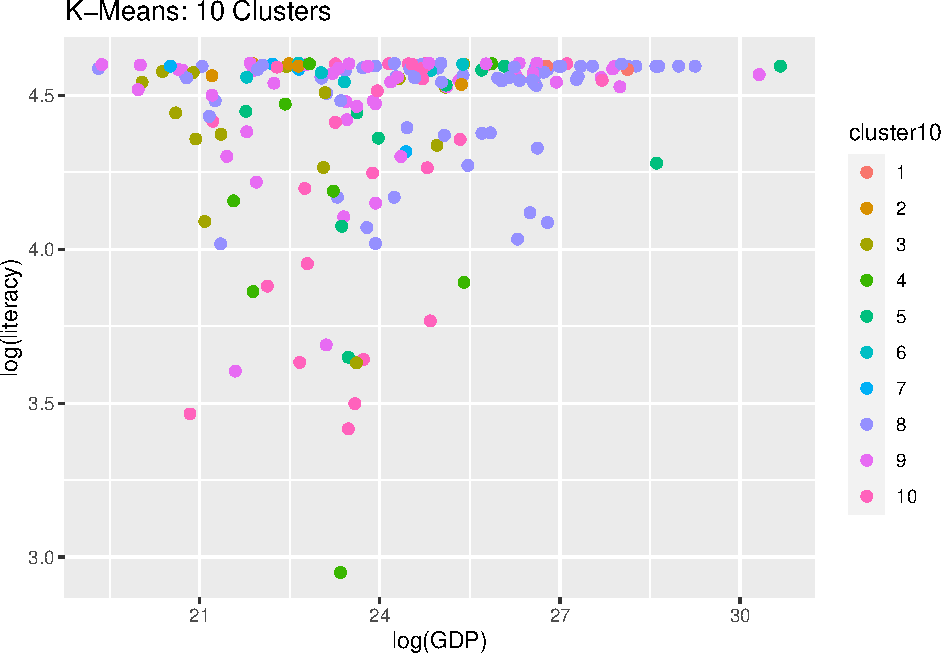
\includegraphics{eda_files/figure-latex/unnamed-chunk-29-4.pdf}

\begin{Shaded}
\begin{Highlighting}[]
\NormalTok{p2 <-}\StringTok{ }\KeywordTok{ggplot}\NormalTok{(master_df_k, }\KeywordTok{aes}\NormalTok{(}\DataTypeTok{x =} \KeywordTok{log}\NormalTok{(GDP), }\DataTypeTok{y =} \KeywordTok{log}\NormalTok{(Expectancy), }\DataTypeTok{color =}\NormalTok{ cluster10)) }\OperatorTok{+}
\StringTok{  }\KeywordTok{geom_point}\NormalTok{(}\DataTypeTok{size=}\DecValTok{2}\NormalTok{)}
\NormalTok{p2 }\OperatorTok{+}\StringTok{ }\KeywordTok{ggtitle}\NormalTok{(}\StringTok{"K-Means: 10 Clusters"}\NormalTok{) }\OperatorTok{+}\StringTok{ }\KeywordTok{scale_fill_brewer}\NormalTok{(}\DataTypeTok{palette=}\StringTok{"Set3"}\NormalTok{)}
\end{Highlighting}
\end{Shaded}

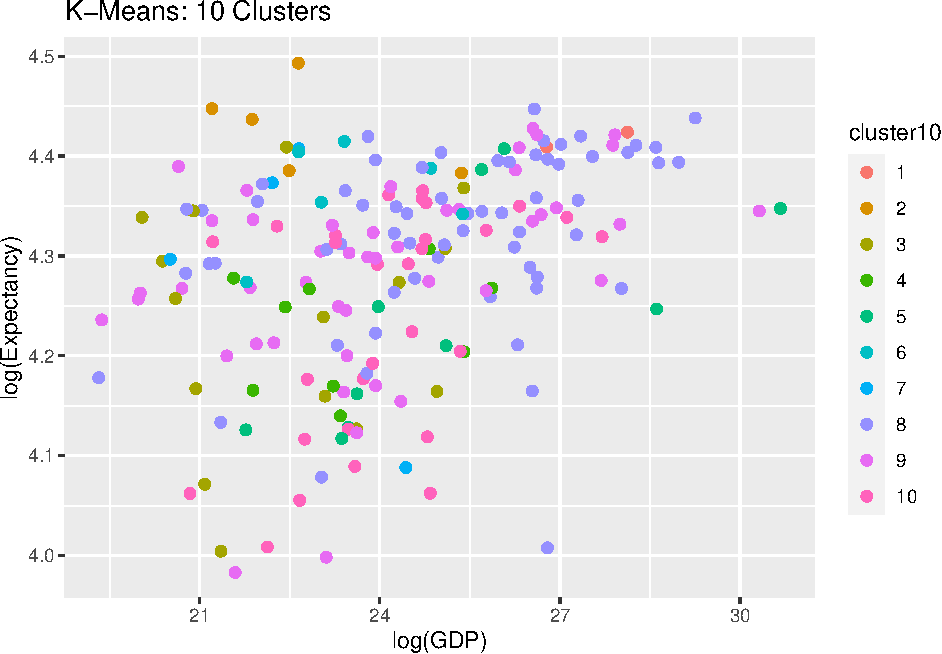
\includegraphics{eda_files/figure-latex/unnamed-chunk-29-5.pdf}

\begin{Shaded}
\begin{Highlighting}[]
\NormalTok{p2 <-}\StringTok{ }\KeywordTok{ggplot}\NormalTok{(master_df_k, }\KeywordTok{aes}\NormalTok{(}\DataTypeTok{x =} \KeywordTok{log}\NormalTok{(Pop), }\DataTypeTok{y =} \KeywordTok{log}\NormalTok{(Expectancy), }\DataTypeTok{color =}\NormalTok{ cluster10)) }\OperatorTok{+}
\StringTok{  }\KeywordTok{geom_point}\NormalTok{(}\DataTypeTok{size=}\DecValTok{2}\NormalTok{)}
\NormalTok{p2 }\OperatorTok{+}\StringTok{ }\KeywordTok{ggtitle}\NormalTok{(}\StringTok{"K-Means: 10 Clusters"}\NormalTok{) }\OperatorTok{+}\StringTok{ }\KeywordTok{scale_fill_brewer}\NormalTok{(}\DataTypeTok{palette=}\StringTok{"Set3"}\NormalTok{)}
\end{Highlighting}
\end{Shaded}

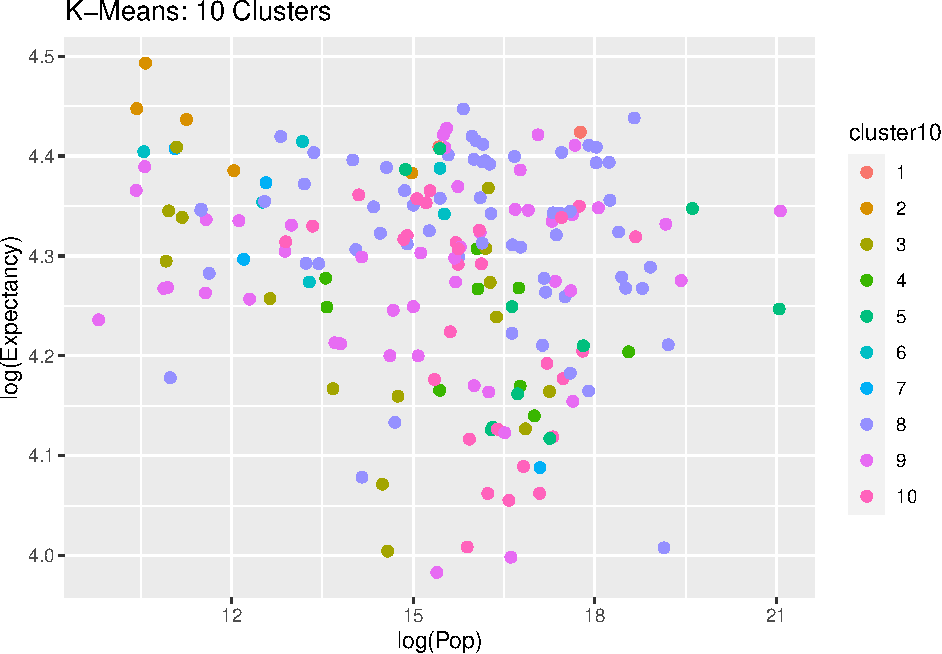
\includegraphics{eda_files/figure-latex/unnamed-chunk-29-6.pdf}

\begin{Shaded}
\begin{Highlighting}[]
\NormalTok{p2 <-}\StringTok{ }\KeywordTok{ggplot}\NormalTok{(master_df_k, }\KeywordTok{aes}\NormalTok{(}\DataTypeTok{x =} \KeywordTok{log}\NormalTok{(Pop), }\DataTypeTok{y =} \KeywordTok{log}\NormalTok{(Fertility), }\DataTypeTok{color =}\NormalTok{ cluster10)) }\OperatorTok{+}
\StringTok{  }\KeywordTok{geom_point}\NormalTok{(}\DataTypeTok{size=}\DecValTok{2}\NormalTok{)}
\NormalTok{p2 }\OperatorTok{+}\StringTok{ }\KeywordTok{ggtitle}\NormalTok{(}\StringTok{"K-Means: 10 Clusters"}\NormalTok{) }\OperatorTok{+}\StringTok{ }\KeywordTok{scale_fill_brewer}\NormalTok{(}\DataTypeTok{palette=}\StringTok{"Set3"}\NormalTok{)}
\end{Highlighting}
\end{Shaded}

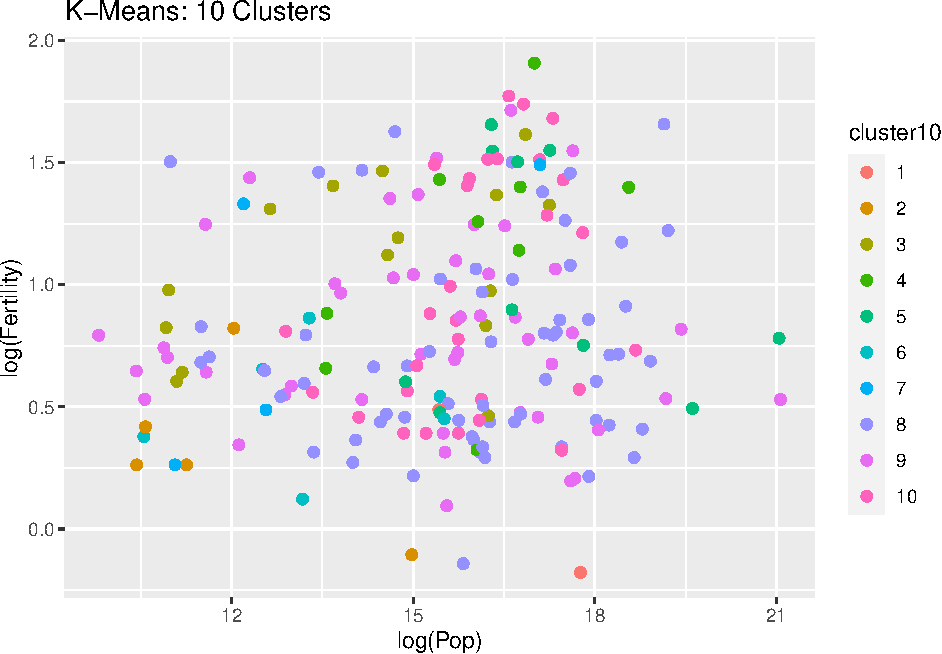
\includegraphics{eda_files/figure-latex/unnamed-chunk-29-7.pdf}

\begin{Shaded}
\begin{Highlighting}[]
\NormalTok{p2 <-}\StringTok{ }\KeywordTok{ggplot}\NormalTok{(master_df_k, }\KeywordTok{aes}\NormalTok{(}\DataTypeTok{x =} \KeywordTok{log}\NormalTok{(Pop), }\DataTypeTok{y =} \KeywordTok{log}\NormalTok{(literacy), }\DataTypeTok{color =}\NormalTok{ cluster10)) }\OperatorTok{+}
\StringTok{  }\KeywordTok{geom_point}\NormalTok{(}\DataTypeTok{size=}\DecValTok{2}\NormalTok{)}
\NormalTok{p2 }\OperatorTok{+}\StringTok{ }\KeywordTok{ggtitle}\NormalTok{(}\StringTok{"K-Means: 10 Clusters"}\NormalTok{) }\OperatorTok{+}\StringTok{ }\KeywordTok{scale_fill_brewer}\NormalTok{(}\DataTypeTok{palette=}\StringTok{"Set3"}\NormalTok{)}
\end{Highlighting}
\end{Shaded}

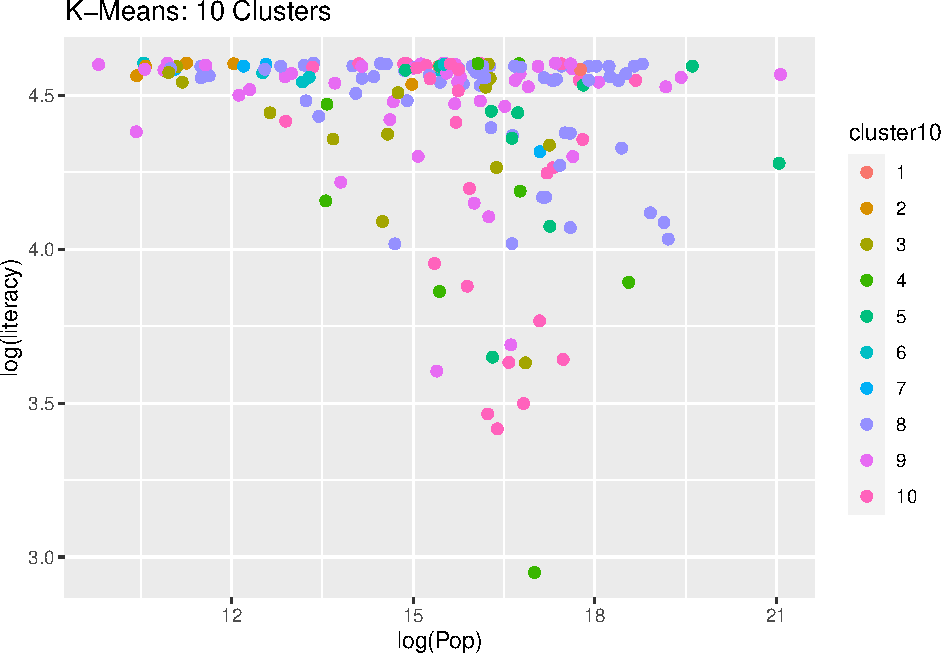
\includegraphics{eda_files/figure-latex/unnamed-chunk-29-8.pdf}

\begin{Shaded}
\begin{Highlighting}[]
\NormalTok{p2 <-}\StringTok{ }\KeywordTok{ggplot}\NormalTok{(master_df_k, }\KeywordTok{aes}\NormalTok{(}\DataTypeTok{x =} \KeywordTok{log}\NormalTok{(Expectancy), }\DataTypeTok{y =} \KeywordTok{log}\NormalTok{(Fertility), }\DataTypeTok{color =}\NormalTok{ cluster10)) }\OperatorTok{+}
\StringTok{  }\KeywordTok{geom_point}\NormalTok{(}\DataTypeTok{size=}\DecValTok{2}\NormalTok{)}
\NormalTok{p2 }\OperatorTok{+}\StringTok{ }\KeywordTok{ggtitle}\NormalTok{(}\StringTok{"K-Means: 10 Clusters"}\NormalTok{) }\OperatorTok{+}\StringTok{ }\KeywordTok{scale_fill_brewer}\NormalTok{(}\DataTypeTok{palette=}\StringTok{"Set3"}\NormalTok{)}
\end{Highlighting}
\end{Shaded}

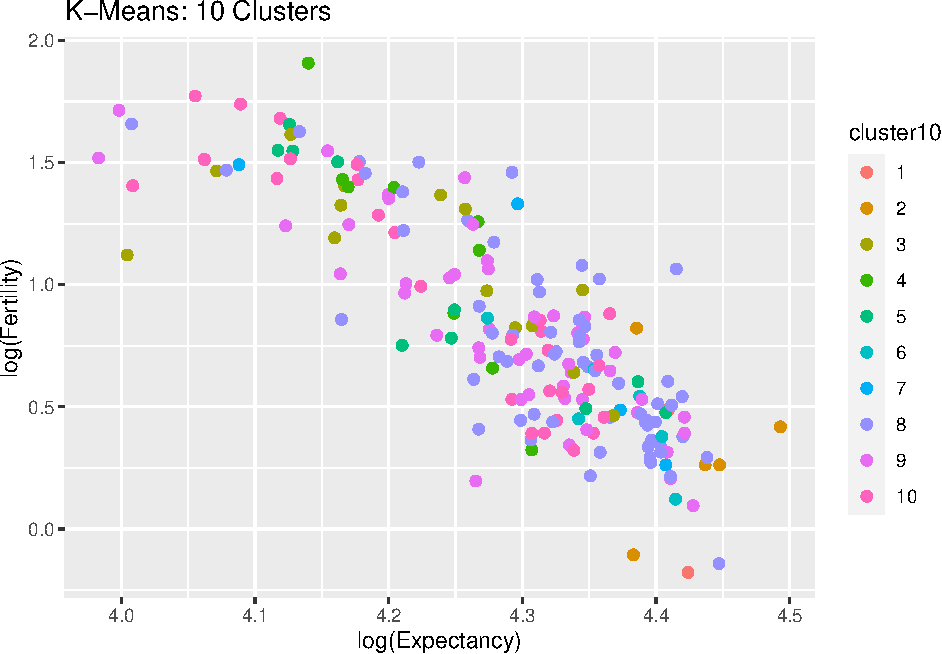
\includegraphics{eda_files/figure-latex/unnamed-chunk-29-9.pdf}

\begin{Shaded}
\begin{Highlighting}[]
\NormalTok{p2 <-}\StringTok{ }\KeywordTok{ggplot}\NormalTok{(master_df_k, }\KeywordTok{aes}\NormalTok{(}\DataTypeTok{x =} \KeywordTok{log}\NormalTok{(Fertility), }\DataTypeTok{y =} \KeywordTok{log}\NormalTok{(literacy), }\DataTypeTok{color =}\NormalTok{ cluster10)) }\OperatorTok{+}
\StringTok{  }\KeywordTok{geom_point}\NormalTok{(}\DataTypeTok{size=}\DecValTok{2}\NormalTok{)}
\NormalTok{p2 }\OperatorTok{+}\StringTok{ }\KeywordTok{ggtitle}\NormalTok{(}\StringTok{"K-Means: 10 Clusters"}\NormalTok{) }\OperatorTok{+}\StringTok{ }\KeywordTok{scale_fill_brewer}\NormalTok{(}\DataTypeTok{palette=}\StringTok{"Set3"}\NormalTok{)}
\end{Highlighting}
\end{Shaded}

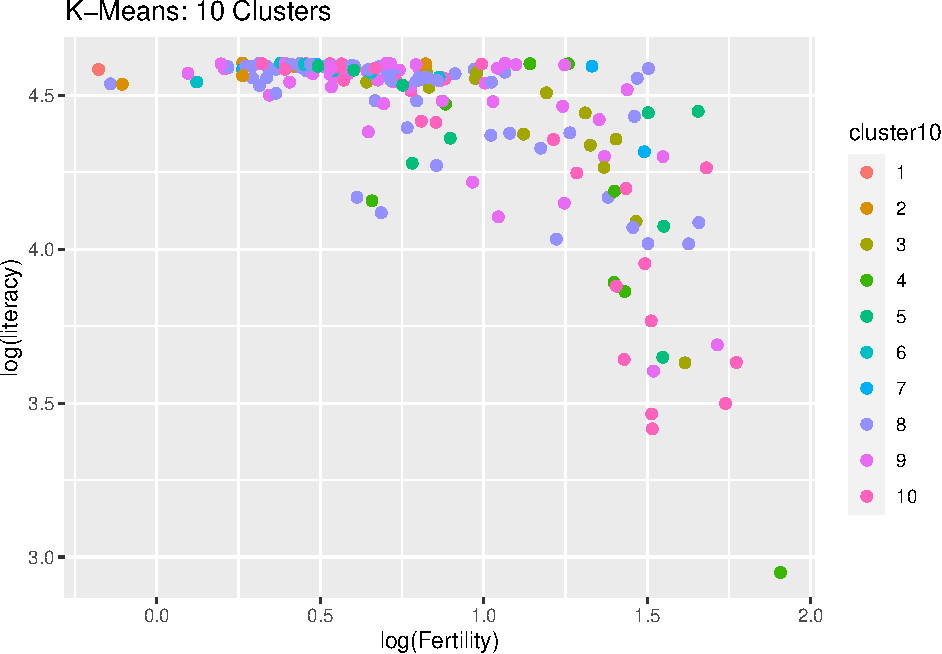
\includegraphics{eda_files/figure-latex/unnamed-chunk-29-10.pdf}

\begin{Shaded}
\begin{Highlighting}[]
\CommentTok{#jpeg(file="kmeans_6.jpg")}
\CommentTok{#dev.off()}

\CommentTok{#jpeg(file="hac_6.jpg")}
\CommentTok{# p3 <- ggplot(master_df_h, aes(x = log(Pop), y = log(Expectancy), color = cluster10)) + geom_point(size=2) }
\CommentTok{# p3 + ggtitle("HAC: 6 Clusters") + scale_fill_brewer(palette="Set3")}
\CommentTok{#dev.off()}
\end{Highlighting}
\end{Shaded}

\begin{Shaded}
\begin{Highlighting}[]
\NormalTok{p2 <-}\StringTok{ }\KeywordTok{ggplot}\NormalTok{(master_df_h, }\KeywordTok{aes}\NormalTok{(}\DataTypeTok{x =} \KeywordTok{log}\NormalTok{(GDP), }\DataTypeTok{y =} \KeywordTok{log}\NormalTok{(Pop), }\DataTypeTok{color =}\NormalTok{ cluster10)) }\OperatorTok{+}
\StringTok{  }\KeywordTok{geom_point}\NormalTok{(}\DataTypeTok{size=}\DecValTok{2}\NormalTok{)}
\NormalTok{p2 }\OperatorTok{+}\StringTok{ }\KeywordTok{ggtitle}\NormalTok{(}\StringTok{"HAC: 10 Clusters"}\NormalTok{) }\OperatorTok{+}\StringTok{ }\KeywordTok{scale_fill_brewer}\NormalTok{(}\DataTypeTok{palette=}\StringTok{"Set3"}\NormalTok{)}
\end{Highlighting}
\end{Shaded}

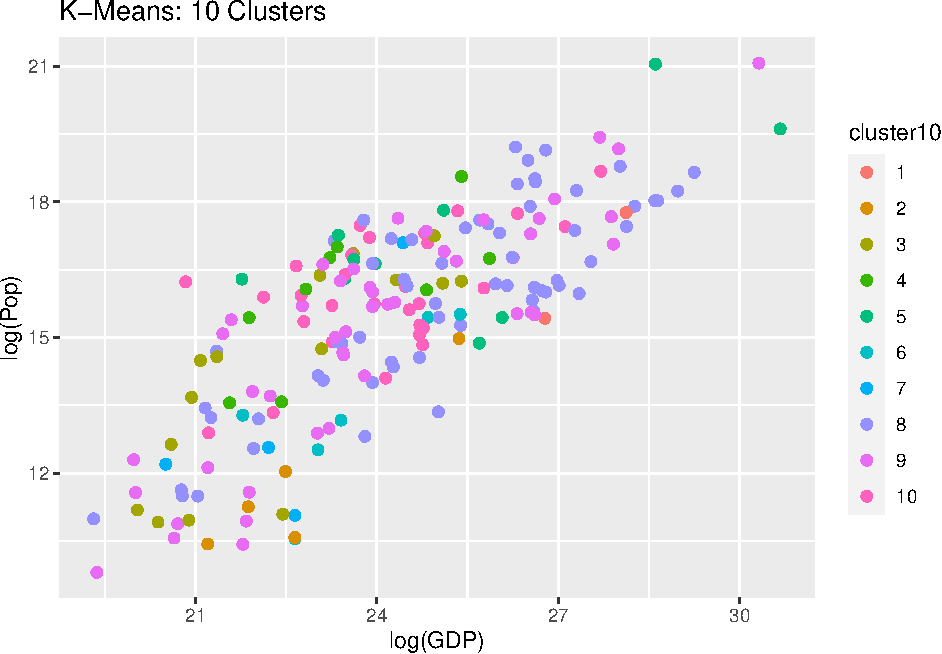
\includegraphics{eda_files/figure-latex/unnamed-chunk-30-1.pdf}

\begin{Shaded}
\begin{Highlighting}[]
\NormalTok{p2 <-}\StringTok{ }\KeywordTok{ggplot}\NormalTok{(master_df_h, }\KeywordTok{aes}\NormalTok{(}\DataTypeTok{x =} \KeywordTok{log}\NormalTok{(GDP), }\DataTypeTok{y =} \KeywordTok{log}\NormalTok{(Expectancy), }\DataTypeTok{color =}\NormalTok{ cluster10)) }\OperatorTok{+}
\StringTok{  }\KeywordTok{geom_point}\NormalTok{(}\DataTypeTok{size=}\DecValTok{2}\NormalTok{)}
\NormalTok{p2 }\OperatorTok{+}\StringTok{ }\KeywordTok{ggtitle}\NormalTok{(}\StringTok{"HAC: 10 Clusters"}\NormalTok{) }\OperatorTok{+}\StringTok{ }\KeywordTok{scale_fill_brewer}\NormalTok{(}\DataTypeTok{palette=}\StringTok{"Set3"}\NormalTok{)}
\end{Highlighting}
\end{Shaded}

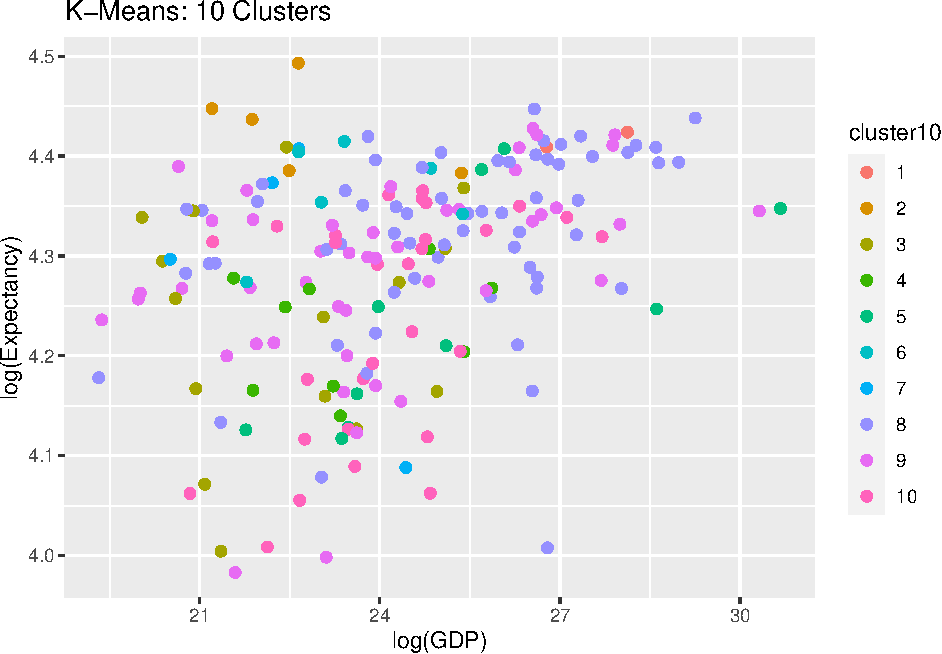
\includegraphics{eda_files/figure-latex/unnamed-chunk-30-2.pdf}

\begin{Shaded}
\begin{Highlighting}[]
\NormalTok{p2 <-}\StringTok{ }\KeywordTok{ggplot}\NormalTok{(master_df_h, }\KeywordTok{aes}\NormalTok{(}\DataTypeTok{x =} \KeywordTok{log}\NormalTok{(GDP), }\DataTypeTok{y =} \KeywordTok{log}\NormalTok{(Fertility), }\DataTypeTok{color =}\NormalTok{ cluster10)) }\OperatorTok{+}
\StringTok{  }\KeywordTok{geom_point}\NormalTok{(}\DataTypeTok{size=}\DecValTok{2}\NormalTok{)}
\NormalTok{p2 }\OperatorTok{+}\StringTok{ }\KeywordTok{ggtitle}\NormalTok{(}\StringTok{"HAC: 10 Clusters"}\NormalTok{) }\OperatorTok{+}\StringTok{ }\KeywordTok{scale_fill_brewer}\NormalTok{(}\DataTypeTok{palette=}\StringTok{"Set3"}\NormalTok{)}
\end{Highlighting}
\end{Shaded}

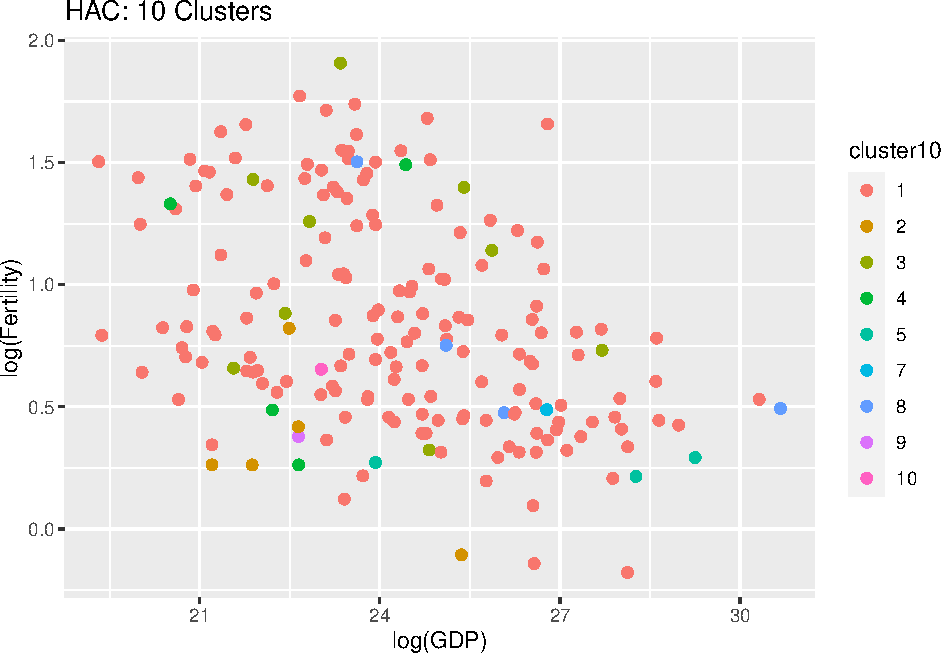
\includegraphics{eda_files/figure-latex/unnamed-chunk-30-3.pdf}

\begin{Shaded}
\begin{Highlighting}[]
\NormalTok{p2 <-}\StringTok{ }\KeywordTok{ggplot}\NormalTok{(master_df_h, }\KeywordTok{aes}\NormalTok{(}\DataTypeTok{x =} \KeywordTok{log}\NormalTok{(GDP), }\DataTypeTok{y =} \KeywordTok{log}\NormalTok{(literacy), }\DataTypeTok{color =}\NormalTok{ cluster10)) }\OperatorTok{+}
\StringTok{  }\KeywordTok{geom_point}\NormalTok{(}\DataTypeTok{size=}\DecValTok{2}\NormalTok{)}
\NormalTok{p2 }\OperatorTok{+}\StringTok{ }\KeywordTok{ggtitle}\NormalTok{(}\StringTok{"HAC: 10 Clusters"}\NormalTok{) }\OperatorTok{+}\StringTok{ }\KeywordTok{scale_fill_brewer}\NormalTok{(}\DataTypeTok{palette=}\StringTok{"Set3"}\NormalTok{)}
\end{Highlighting}
\end{Shaded}

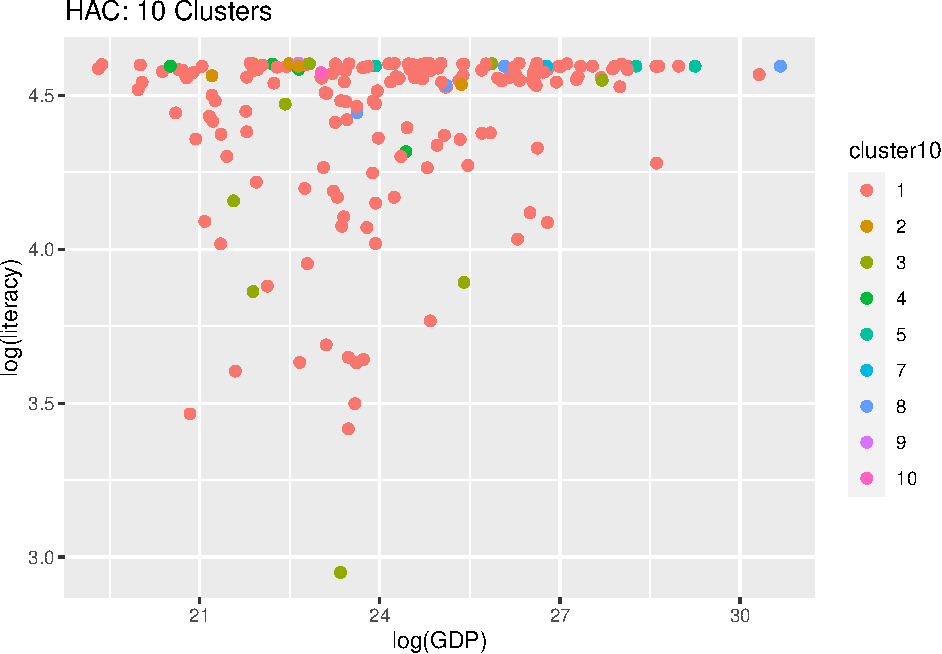
\includegraphics{eda_files/figure-latex/unnamed-chunk-30-4.pdf}

\begin{Shaded}
\begin{Highlighting}[]
\NormalTok{p2 <-}\StringTok{ }\KeywordTok{ggplot}\NormalTok{(master_df_h, }\KeywordTok{aes}\NormalTok{(}\DataTypeTok{x =} \KeywordTok{log}\NormalTok{(GDP), }\DataTypeTok{y =} \KeywordTok{log}\NormalTok{(Expectancy), }\DataTypeTok{color =}\NormalTok{ cluster10)) }\OperatorTok{+}
\StringTok{  }\KeywordTok{geom_point}\NormalTok{(}\DataTypeTok{size=}\DecValTok{2}\NormalTok{)}
\NormalTok{p2 }\OperatorTok{+}\StringTok{ }\KeywordTok{ggtitle}\NormalTok{(}\StringTok{"HAC: 10 Clusters"}\NormalTok{) }\OperatorTok{+}\StringTok{ }\KeywordTok{scale_fill_brewer}\NormalTok{(}\DataTypeTok{palette=}\StringTok{"Set3"}\NormalTok{)}
\end{Highlighting}
\end{Shaded}

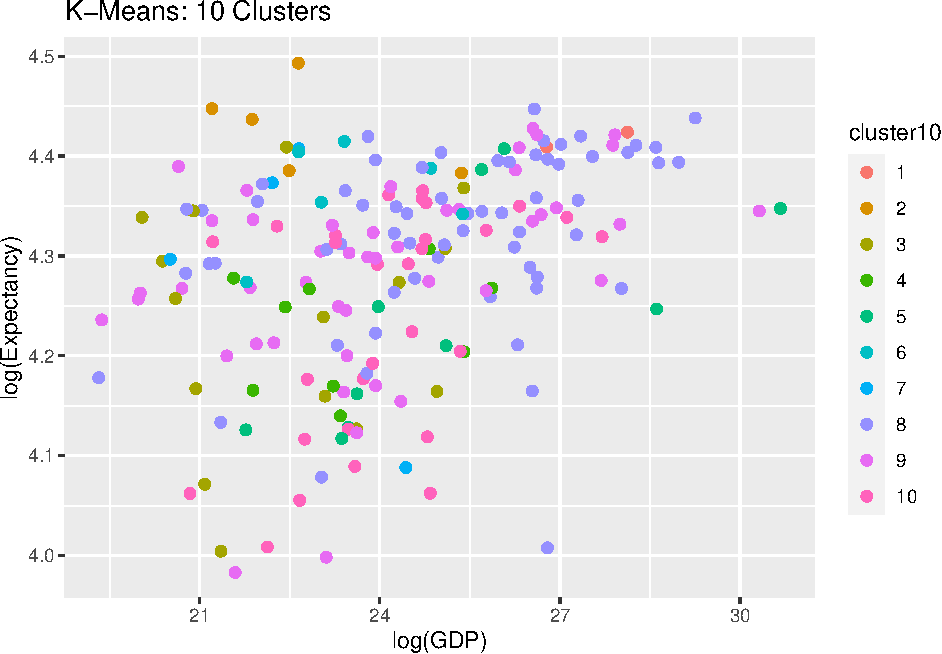
\includegraphics{eda_files/figure-latex/unnamed-chunk-30-5.pdf}

\begin{Shaded}
\begin{Highlighting}[]
\NormalTok{p2 <-}\StringTok{ }\KeywordTok{ggplot}\NormalTok{(master_df_h, }\KeywordTok{aes}\NormalTok{(}\DataTypeTok{x =} \KeywordTok{log}\NormalTok{(Pop), }\DataTypeTok{y =} \KeywordTok{log}\NormalTok{(Expectancy), }\DataTypeTok{color =}\NormalTok{ cluster10)) }\OperatorTok{+}
\StringTok{  }\KeywordTok{geom_point}\NormalTok{(}\DataTypeTok{size=}\DecValTok{2}\NormalTok{)}
\NormalTok{p2 }\OperatorTok{+}\StringTok{ }\KeywordTok{ggtitle}\NormalTok{(}\StringTok{"HAC: 10 Clusters"}\NormalTok{) }\OperatorTok{+}\StringTok{ }\KeywordTok{scale_fill_brewer}\NormalTok{(}\DataTypeTok{palette=}\StringTok{"Set3"}\NormalTok{)}
\end{Highlighting}
\end{Shaded}

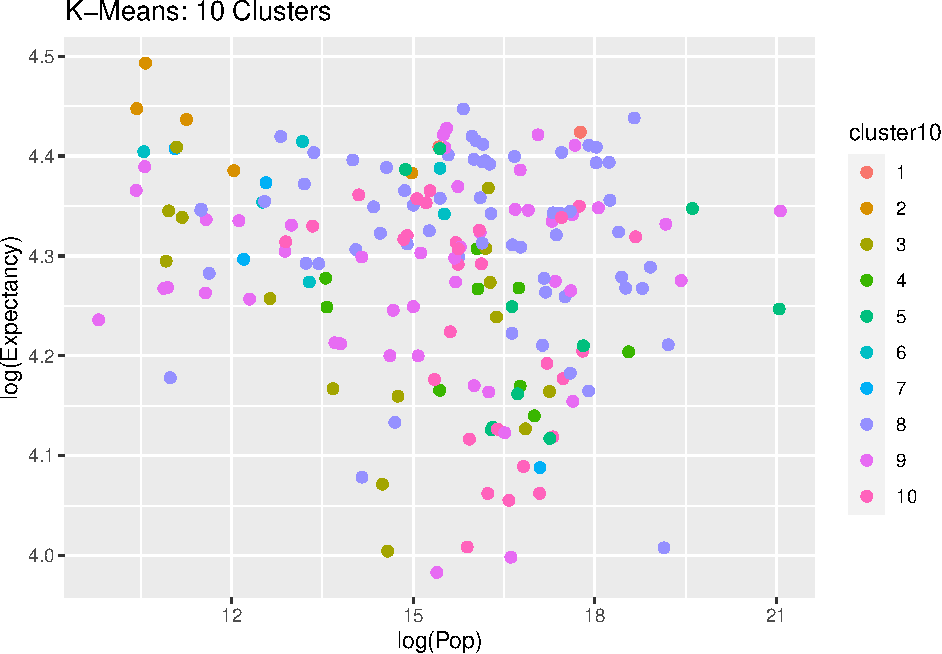
\includegraphics{eda_files/figure-latex/unnamed-chunk-30-6.pdf}

\begin{Shaded}
\begin{Highlighting}[]
\NormalTok{p2 <-}\StringTok{ }\KeywordTok{ggplot}\NormalTok{(master_df_h, }\KeywordTok{aes}\NormalTok{(}\DataTypeTok{x =} \KeywordTok{log}\NormalTok{(Pop), }\DataTypeTok{y =} \KeywordTok{log}\NormalTok{(Fertility), }\DataTypeTok{color =}\NormalTok{ cluster10)) }\OperatorTok{+}
\StringTok{  }\KeywordTok{geom_point}\NormalTok{(}\DataTypeTok{size=}\DecValTok{2}\NormalTok{)}
\NormalTok{p2 }\OperatorTok{+}\StringTok{ }\KeywordTok{ggtitle}\NormalTok{(}\StringTok{"HAC: 10 Clusters"}\NormalTok{) }\OperatorTok{+}\StringTok{ }\KeywordTok{scale_fill_brewer}\NormalTok{(}\DataTypeTok{palette=}\StringTok{"Set3"}\NormalTok{)}
\end{Highlighting}
\end{Shaded}

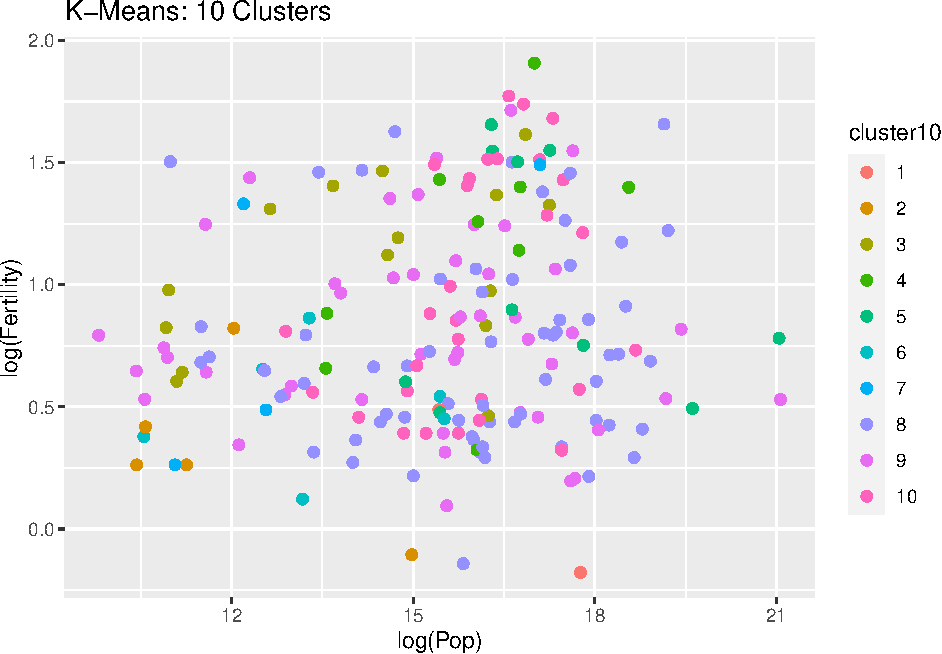
\includegraphics{eda_files/figure-latex/unnamed-chunk-30-7.pdf}

\begin{Shaded}
\begin{Highlighting}[]
\NormalTok{p2 <-}\StringTok{ }\KeywordTok{ggplot}\NormalTok{(master_df_h, }\KeywordTok{aes}\NormalTok{(}\DataTypeTok{x =} \KeywordTok{log}\NormalTok{(Pop), }\DataTypeTok{y =} \KeywordTok{log}\NormalTok{(literacy), }\DataTypeTok{color =}\NormalTok{ cluster10)) }\OperatorTok{+}
\StringTok{  }\KeywordTok{geom_point}\NormalTok{(}\DataTypeTok{size=}\DecValTok{2}\NormalTok{)}
\NormalTok{p2 }\OperatorTok{+}\StringTok{ }\KeywordTok{ggtitle}\NormalTok{(}\StringTok{"HAC: 10 Clusters"}\NormalTok{) }\OperatorTok{+}\StringTok{ }\KeywordTok{scale_fill_brewer}\NormalTok{(}\DataTypeTok{palette=}\StringTok{"Set3"}\NormalTok{)}
\end{Highlighting}
\end{Shaded}

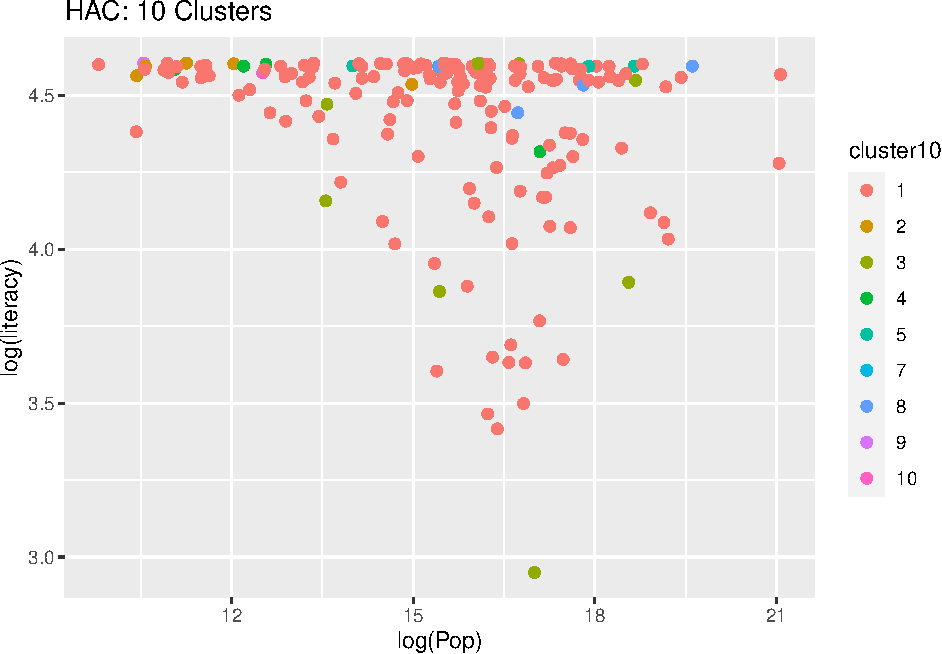
\includegraphics{eda_files/figure-latex/unnamed-chunk-30-8.pdf}

\begin{Shaded}
\begin{Highlighting}[]
\NormalTok{p2 <-}\StringTok{ }\KeywordTok{ggplot}\NormalTok{(master_df_h, }\KeywordTok{aes}\NormalTok{(}\DataTypeTok{x =} \KeywordTok{log}\NormalTok{(Expectancy), }\DataTypeTok{y =} \KeywordTok{log}\NormalTok{(Fertility), }\DataTypeTok{color =}\NormalTok{ cluster10)) }\OperatorTok{+}
\StringTok{  }\KeywordTok{geom_point}\NormalTok{(}\DataTypeTok{size=}\DecValTok{2}\NormalTok{)}
\NormalTok{p2 }\OperatorTok{+}\StringTok{ }\KeywordTok{ggtitle}\NormalTok{(}\StringTok{"HAC: 10 Clusters"}\NormalTok{) }\OperatorTok{+}\StringTok{ }\KeywordTok{scale_fill_brewer}\NormalTok{(}\DataTypeTok{palette=}\StringTok{"Set3"}\NormalTok{)}
\end{Highlighting}
\end{Shaded}

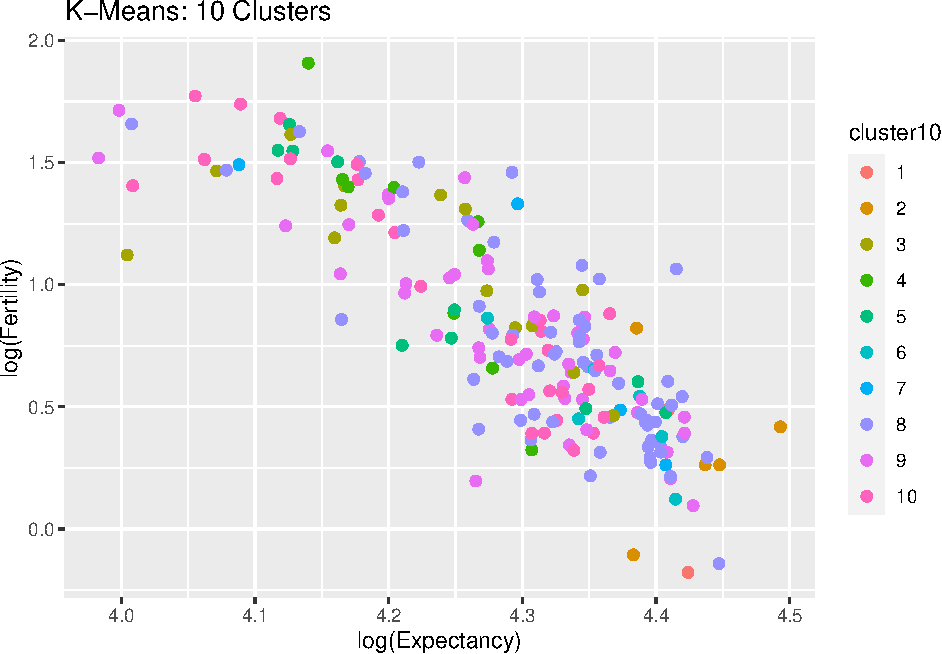
\includegraphics{eda_files/figure-latex/unnamed-chunk-30-9.pdf}

\begin{Shaded}
\begin{Highlighting}[]
\NormalTok{p2 <-}\StringTok{ }\KeywordTok{ggplot}\NormalTok{(master_df_h, }\KeywordTok{aes}\NormalTok{(}\DataTypeTok{x =} \KeywordTok{log}\NormalTok{(Fertility), }\DataTypeTok{y =} \KeywordTok{log}\NormalTok{(literacy), }\DataTypeTok{color =}\NormalTok{ cluster10)) }\OperatorTok{+}
\StringTok{  }\KeywordTok{geom_point}\NormalTok{(}\DataTypeTok{size=}\DecValTok{2}\NormalTok{)}
\NormalTok{p2 }\OperatorTok{+}\StringTok{ }\KeywordTok{ggtitle}\NormalTok{(}\StringTok{"HAC: 10 Clusters"}\NormalTok{) }\OperatorTok{+}\StringTok{ }\KeywordTok{scale_fill_brewer}\NormalTok{(}\DataTypeTok{palette=}\StringTok{"Set3"}\NormalTok{)}
\end{Highlighting}
\end{Shaded}

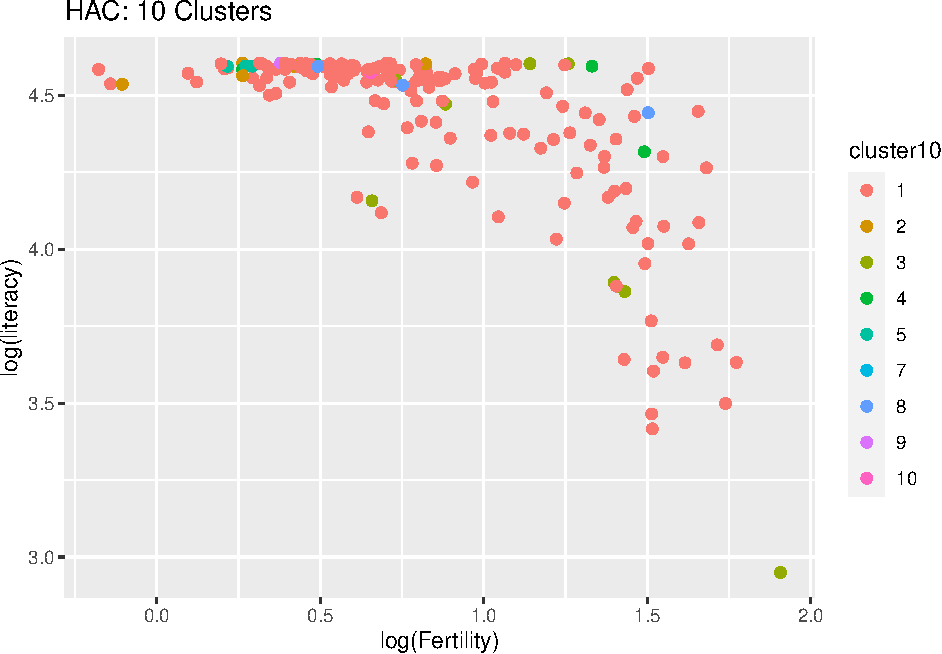
\includegraphics{eda_files/figure-latex/unnamed-chunk-30-10.pdf}

\begin{Shaded}
\begin{Highlighting}[]
\CommentTok{# not sure how meaningful something like this would be? definitely needs some cleaning up}
\CommentTok{# source of code: https://stackoverflow.com/questions/47842646/labelling-outliers-with-ggplot}
\KeywordTok{jpeg}\NormalTok{(}\DataTypeTok{file=}\StringTok{"boxplot_k_literacy.jpg"}\NormalTok{)}
\KeywordTok{ggplot}\NormalTok{(master_df_k, }\KeywordTok{aes}\NormalTok{(}\DataTypeTok{x =}\NormalTok{ cluster10, }\DataTypeTok{y =}\NormalTok{ literacy, }\DataTypeTok{fill =}\NormalTok{ cluster10)) }\OperatorTok{+}
\StringTok{  }\KeywordTok{geom_boxplot}\NormalTok{(}\DataTypeTok{alpha =} \FloatTok{0.3}\NormalTok{) }\OperatorTok{+}
\StringTok{  }\KeywordTok{geom_point}\NormalTok{(}\KeywordTok{aes}\NormalTok{(}\DataTypeTok{color =}\NormalTok{ cluster10, }\DataTypeTok{group =}\NormalTok{ cluster10), }\DataTypeTok{position =} \KeywordTok{position_dodge}\NormalTok{(}\DataTypeTok{width=}\FloatTok{0.75}\NormalTok{)) }\OperatorTok{+}
\StringTok{  }\KeywordTok{geom_text_repel}\NormalTok{(}\KeywordTok{aes}\NormalTok{(}\DataTypeTok{group =}\NormalTok{ cluster10, }
                \DataTypeTok{label =} \KeywordTok{ifelse}\NormalTok{(}\DataTypeTok{test =}\NormalTok{ literacy }\OperatorTok{>}\StringTok{ }\KeywordTok{median}\NormalTok{(literacy) }\OperatorTok{+}\StringTok{ }\FloatTok{1.5}\OperatorTok{*}\KeywordTok{IQR}\NormalTok{(literacy)}
                               \OperatorTok{|}\StringTok{ }\NormalTok{literacy }\OperatorTok{<}\StringTok{ }\KeywordTok{median}\NormalTok{(literacy) }\OperatorTok{-}\StringTok{ }\FloatTok{1.5}\OperatorTok{*}\KeywordTok{IQR}\NormalTok{(literacy), }
                  \DataTypeTok{yes =}\NormalTok{ ISO3,}
                  \DataTypeTok{no =} \StringTok{''}\NormalTok{)), }
            \DataTypeTok{position =} \KeywordTok{position_dodge}\NormalTok{(}\DataTypeTok{width=}\FloatTok{0.75}\NormalTok{),}
            \DataTypeTok{hjust =} \StringTok{"left"}\NormalTok{, }\DataTypeTok{size =} \DecValTok{3}\NormalTok{) }\OperatorTok{+}\StringTok{ }\KeywordTok{ggtitle}\NormalTok{(}\StringTok{"HAC GDP Boxplot"}\NormalTok{) }\OperatorTok{+}\StringTok{ }\KeywordTok{xlab}\NormalTok{(}\StringTok{"Policy Cluster"}\NormalTok{) }\OperatorTok{+}\StringTok{ }
\StringTok{  }\KeywordTok{theme}\NormalTok{(}\DataTypeTok{legend.position =} \StringTok{"none"}\NormalTok{)}
\KeywordTok{dev.off}\NormalTok{()}
\end{Highlighting}
\end{Shaded}

\begin{verbatim}
## pdf 
##   2
\end{verbatim}

\begin{Shaded}
\begin{Highlighting}[]
\KeywordTok{jpeg}\NormalTok{(}\DataTypeTok{file=}\StringTok{"boxplot_k_fertility.jpg"}\NormalTok{)}
\KeywordTok{ggplot}\NormalTok{(master_df_k, }\KeywordTok{aes}\NormalTok{(}\DataTypeTok{x =}\NormalTok{ cluster10, }\DataTypeTok{y =}\NormalTok{ Fertility, }\DataTypeTok{fill =}\NormalTok{ cluster10)) }\OperatorTok{+}
\StringTok{  }\KeywordTok{geom_boxplot}\NormalTok{(}\DataTypeTok{alpha =} \FloatTok{0.3}\NormalTok{) }\OperatorTok{+}
\StringTok{  }\KeywordTok{geom_point}\NormalTok{(}\KeywordTok{aes}\NormalTok{(}\DataTypeTok{color =}\NormalTok{ cluster10, }\DataTypeTok{group =}\NormalTok{ cluster10), }\DataTypeTok{position =} \KeywordTok{position_dodge}\NormalTok{(}\DataTypeTok{width=}\FloatTok{0.75}\NormalTok{)) }\OperatorTok{+}
\StringTok{  }\KeywordTok{geom_text_repel}\NormalTok{(}\KeywordTok{aes}\NormalTok{(}\DataTypeTok{group =}\NormalTok{ cluster10, }
                \DataTypeTok{label =} \KeywordTok{ifelse}\NormalTok{(}\DataTypeTok{test =}\NormalTok{ Fertility }\OperatorTok{>}\StringTok{ }\KeywordTok{median}\NormalTok{(Fertility) }\OperatorTok{+}\StringTok{ }\FloatTok{1.5}\OperatorTok{*}\KeywordTok{IQR}\NormalTok{(Fertility)}
                               \OperatorTok{|}\StringTok{ }\NormalTok{Fertility }\OperatorTok{<}\StringTok{ }\KeywordTok{median}\NormalTok{(Fertility) }\OperatorTok{-}\StringTok{ }\FloatTok{1.5}\OperatorTok{*}\KeywordTok{IQR}\NormalTok{(Fertility), }
                  \DataTypeTok{yes =}\NormalTok{ ISO3,}
                  \DataTypeTok{no =} \StringTok{''}\NormalTok{)), }
            \DataTypeTok{position =} \KeywordTok{position_dodge}\NormalTok{(}\DataTypeTok{width=}\FloatTok{0.75}\NormalTok{),}
            \DataTypeTok{hjust =} \StringTok{"left"}\NormalTok{, }\DataTypeTok{size =} \DecValTok{3}\NormalTok{) }\OperatorTok{+}\StringTok{ }\KeywordTok{ggtitle}\NormalTok{(}\StringTok{"HAC GDP Boxplot"}\NormalTok{) }\OperatorTok{+}\StringTok{ }\KeywordTok{xlab}\NormalTok{(}\StringTok{"Policy Cluster"}\NormalTok{) }\OperatorTok{+}\StringTok{ }
\StringTok{  }\KeywordTok{theme}\NormalTok{(}\DataTypeTok{legend.position =} \StringTok{"none"}\NormalTok{)}

\KeywordTok{dev.off}\NormalTok{()}
\end{Highlighting}
\end{Shaded}

\begin{verbatim}
## pdf 
##   2
\end{verbatim}

\begin{Shaded}
\begin{Highlighting}[]
\KeywordTok{jpeg}\NormalTok{(}\DataTypeTok{file=}\StringTok{"boxplot_h_gdp.jpg"}\NormalTok{)}
\KeywordTok{ggplot}\NormalTok{(master_df_h[}\OperatorTok{!}\KeywordTok{is.na}\NormalTok{(master_df_h}\OperatorTok{$}\NormalTok{GDP), ], }\KeywordTok{aes}\NormalTok{(}\DataTypeTok{x =}\NormalTok{ cluster10, }\DataTypeTok{y =} \KeywordTok{log}\NormalTok{(GDP), }\DataTypeTok{fill =} 
\NormalTok{                                                     cluster10)) }\OperatorTok{+}
\StringTok{  }\KeywordTok{geom_boxplot}\NormalTok{(}\DataTypeTok{alpha =} \FloatTok{0.3}\NormalTok{) }\OperatorTok{+}
\StringTok{  }\KeywordTok{geom_point}\NormalTok{(}\KeywordTok{aes}\NormalTok{(}\DataTypeTok{color =}\NormalTok{ cluster10, }\DataTypeTok{group =}\NormalTok{ cluster10), }\DataTypeTok{position =} \KeywordTok{position_dodge}\NormalTok{(}\DataTypeTok{width=}\FloatTok{0.75}\NormalTok{)) }\OperatorTok{+}
\StringTok{  }\KeywordTok{geom_text_repel}\NormalTok{(}\KeywordTok{aes}\NormalTok{(}\DataTypeTok{group =}\NormalTok{ cluster10, }
                \DataTypeTok{label =} \KeywordTok{ifelse}\NormalTok{(}\DataTypeTok{test =} \KeywordTok{log}\NormalTok{(GDP) }\OperatorTok{>}\StringTok{ }\KeywordTok{median}\NormalTok{(}\KeywordTok{log}\NormalTok{(GDP)) }\OperatorTok{+}\StringTok{ }\FloatTok{1.5}\OperatorTok{*}\KeywordTok{IQR}\NormalTok{(}\KeywordTok{log}\NormalTok{(GDP))}
                               \OperatorTok{|}\StringTok{ }\KeywordTok{log}\NormalTok{(GDP) }\OperatorTok{<}\StringTok{ }\KeywordTok{median}\NormalTok{(}\KeywordTok{log}\NormalTok{(GDP)) }\OperatorTok{-}\StringTok{ }\FloatTok{1.5}\OperatorTok{*}\KeywordTok{IQR}\NormalTok{(}\KeywordTok{log}\NormalTok{(GDP)), }
                  \DataTypeTok{yes =}\NormalTok{ ISO3,}
                  \DataTypeTok{no =} \StringTok{''}\NormalTok{)), }
            \DataTypeTok{position =} \KeywordTok{position_dodge}\NormalTok{(}\DataTypeTok{width=}\FloatTok{0.75}\NormalTok{),}
            \DataTypeTok{hjust =} \StringTok{"left"}\NormalTok{, }\DataTypeTok{size =} \DecValTok{3}\NormalTok{) }\OperatorTok{+}
\StringTok{  }\KeywordTok{ggtitle}\NormalTok{(}\StringTok{"HAC GDP Boxplot"}\NormalTok{) }\OperatorTok{+}\StringTok{ }\KeywordTok{xlab}\NormalTok{(}\StringTok{"Policy Cluster"}\NormalTok{) }\OperatorTok{+}\StringTok{ }\KeywordTok{theme}\NormalTok{(}\DataTypeTok{legend.position =} \StringTok{"none"}\NormalTok{)}
\KeywordTok{dev.off}\NormalTok{()}
\end{Highlighting}
\end{Shaded}

\begin{verbatim}
## pdf 
##   2
\end{verbatim}

\begin{Shaded}
\begin{Highlighting}[]
\CommentTok{# ggrepel}
\CommentTok{# deal with missing data}
\end{Highlighting}
\end{Shaded}

\begin{Shaded}
\begin{Highlighting}[]
\KeywordTok{jpeg}\NormalTok{(}\DataTypeTok{file =} \StringTok{"boxplot_k_expectancy.jpg"}\NormalTok{)}
\KeywordTok{ggplot}\NormalTok{(master_df_k, }
       \KeywordTok{aes}\NormalTok{(}\DataTypeTok{x =}\NormalTok{ cluster10, }\DataTypeTok{y =}\NormalTok{ Expectancy, }\DataTypeTok{fill =}\NormalTok{ cluster10)) }\OperatorTok{+}
\StringTok{  }\KeywordTok{geom_boxplot}\NormalTok{(}\DataTypeTok{alpha =} \FloatTok{0.3}\NormalTok{) }\OperatorTok{+}
\StringTok{  }\KeywordTok{geom_point}\NormalTok{(}\KeywordTok{aes}\NormalTok{(}\DataTypeTok{color =}\NormalTok{ cluster10, }\DataTypeTok{group =}\NormalTok{ cluster10), }\DataTypeTok{position =} \KeywordTok{position_dodge}\NormalTok{(}\DataTypeTok{width=}\FloatTok{0.75}\NormalTok{)) }\OperatorTok{+}
\StringTok{  }\KeywordTok{geom_text_repel}\NormalTok{(}\KeywordTok{aes}\NormalTok{(}\DataTypeTok{group =}\NormalTok{ cluster10, }
                \DataTypeTok{label =} \KeywordTok{ifelse}\NormalTok{(}\DataTypeTok{test =}\NormalTok{ Expectancy }\OperatorTok{>}\StringTok{ }\KeywordTok{median}\NormalTok{(Expectancy)}
                               \OperatorTok{+}\StringTok{ }\FloatTok{1.5}\OperatorTok{*}\KeywordTok{IQR}\NormalTok{(Expectancy) }\OperatorTok{|}\StringTok{ }\NormalTok{Expectancy }\OperatorTok{<}\StringTok{ }
\StringTok{                                 }\KeywordTok{median}\NormalTok{(Expectancy) }\OperatorTok{-}\StringTok{ }\FloatTok{1.5}\OperatorTok{*}\KeywordTok{IQR}\NormalTok{(Expectancy), }
                  \DataTypeTok{yes =}\NormalTok{ ISO3,}
                  \DataTypeTok{no =} \StringTok{''}\NormalTok{)), }
            \DataTypeTok{position =} \KeywordTok{position_dodge}\NormalTok{(}\DataTypeTok{width=}\FloatTok{0.75}\NormalTok{),}
            \DataTypeTok{hjust =} \StringTok{"left"}\NormalTok{, }\DataTypeTok{size =} \DecValTok{3}\NormalTok{) }\OperatorTok{+}\StringTok{ }\KeywordTok{ggtitle}\NormalTok{(}\StringTok{"HAC GDP Boxplot"}\NormalTok{) }\OperatorTok{+}\StringTok{ }
\StringTok{  }\KeywordTok{xlab}\NormalTok{(}\StringTok{"Policy Cluster"}\NormalTok{) }\OperatorTok{+}\StringTok{ }\KeywordTok{theme}\NormalTok{(}\DataTypeTok{legend.position =} \StringTok{"none"}\NormalTok{)}
\KeywordTok{dev.off}\NormalTok{()}
\end{Highlighting}
\end{Shaded}

\begin{verbatim}
## pdf 
##   2
\end{verbatim}

\begin{Shaded}
\begin{Highlighting}[]
\CommentTok{## BOXPLOT QUESTIONS}
\KeywordTok{jpeg}\NormalTok{(}\DataTypeTok{file =} \StringTok{"boxplot_h_expectancy.jpg"}\NormalTok{)}
\KeywordTok{ggplot}\NormalTok{(master_df_h, }
       \KeywordTok{aes}\NormalTok{(}\DataTypeTok{x =}\NormalTok{ cluster10, }\DataTypeTok{y =}\NormalTok{ Expectancy, }\DataTypeTok{fill =}\NormalTok{ cluster10)) }\OperatorTok{+}
\StringTok{  }\KeywordTok{geom_boxplot}\NormalTok{(}\DataTypeTok{alpha =} \FloatTok{0.3}\NormalTok{) }\OperatorTok{+}
\StringTok{  }\KeywordTok{geom_point}\NormalTok{(}\KeywordTok{aes}\NormalTok{(}\DataTypeTok{color =}\NormalTok{ cluster10, }\DataTypeTok{group =}\NormalTok{ cluster10), }\DataTypeTok{position =} \KeywordTok{position_dodge}\NormalTok{(}\DataTypeTok{width=}\FloatTok{0.75}\NormalTok{)) }\OperatorTok{+}
\StringTok{  }\KeywordTok{geom_text_repel}\NormalTok{(}\KeywordTok{aes}\NormalTok{(}\DataTypeTok{group =}\NormalTok{ cluster10, }
                \DataTypeTok{label =} \KeywordTok{ifelse}\NormalTok{(}\DataTypeTok{test =}\NormalTok{ Expectancy }\OperatorTok{>}\StringTok{ }\KeywordTok{median}\NormalTok{(Expectancy)}
                               \OperatorTok{+}\StringTok{ }\FloatTok{1.5}\OperatorTok{*}\KeywordTok{IQR}\NormalTok{(Expectancy) }\OperatorTok{|}\StringTok{ }\NormalTok{Expectancy }\OperatorTok{<}\StringTok{ }
\StringTok{                                 }\KeywordTok{median}\NormalTok{(Expectancy) }\OperatorTok{-}\StringTok{ }\FloatTok{1.5}\OperatorTok{*}\KeywordTok{IQR}\NormalTok{(Expectancy), }
                  \DataTypeTok{yes =}\NormalTok{ ISO3,}
                  \DataTypeTok{no =} \StringTok{''}\NormalTok{)), }
            \DataTypeTok{position =} \KeywordTok{position_dodge}\NormalTok{(}\DataTypeTok{width=}\FloatTok{0.75}\NormalTok{),}
            \DataTypeTok{hjust =} \StringTok{"left"}\NormalTok{, }\DataTypeTok{size =} \DecValTok{3}\NormalTok{) }\OperatorTok{+}\StringTok{ }\KeywordTok{ggtitle}\NormalTok{(}\StringTok{"HAC GDP Boxplot"}\NormalTok{) }\OperatorTok{+}\StringTok{ }\KeywordTok{xlab}\NormalTok{(}\StringTok{"Policy Cluster"}\NormalTok{) }\OperatorTok{+}\StringTok{ }
\StringTok{  }\KeywordTok{theme}\NormalTok{(}\DataTypeTok{legend.position =} \StringTok{"none"}\NormalTok{)}
\KeywordTok{dev.off}\NormalTok{()}
\end{Highlighting}
\end{Shaded}

\begin{verbatim}
## pdf 
##   2
\end{verbatim}

\begin{Shaded}
\begin{Highlighting}[]
\NormalTok{iso3}\OperatorTok{$}\NormalTok{Alpha.}\FloatTok{3.}\NormalTok{code <-}\StringTok{ }\KeywordTok{trimws}\NormalTok{(iso3}\OperatorTok{$}\NormalTok{Alpha.}\FloatTok{3.}\NormalTok{code)}
\NormalTok{names_h <-}\StringTok{ }\KeywordTok{merge}\NormalTok{(master_df_h, iso3, }\DataTypeTok{by.x =} \StringTok{"ISO3"}\NormalTok{, }\DataTypeTok{by.y =} \StringTok{"Alpha.3.code"}\NormalTok{)}
\NormalTok{names_k <-}\StringTok{ }\KeywordTok{merge}\NormalTok{(master_df_k, iso3, }\DataTypeTok{by.x =} \StringTok{"ISO3"}\NormalTok{, }\DataTypeTok{by.y =} \StringTok{"Alpha.3.code"}\NormalTok{)}
\NormalTok{countries_h <-}\StringTok{ }\KeywordTok{data.frame}\NormalTok{()}
\NormalTok{countries_k <-}\StringTok{ }\KeywordTok{rep}\NormalTok{(}\OtherTok{NA}\NormalTok{, }\DecValTok{10}\NormalTok{)}
\ControlFlowTok{for}\NormalTok{ (i }\ControlFlowTok{in} \DecValTok{1}\OperatorTok{:}\DecValTok{10}\NormalTok{) \{}
\NormalTok{  names_h[names_h}\OperatorTok{$}\NormalTok{cluster10 }\OperatorTok{==}\StringTok{ }\NormalTok{i, ]}\OperatorTok{$}\NormalTok{Country}
\NormalTok{  names_h[names_k}\OperatorTok{$}\NormalTok{cluster10 }\OperatorTok{==}\StringTok{ }\NormalTok{i, ]}\OperatorTok{$}\NormalTok{Country}
\NormalTok{\}}
\end{Highlighting}
\end{Shaded}

\begin{Shaded}
\begin{Highlighting}[]
\CommentTok{#appendix (use xtable to format into Latex)}
\CommentTok{# kableExtra}
\NormalTok{tb <-}\StringTok{ }\KeywordTok{split}\NormalTok{(master_df_k, master_df_k}\OperatorTok{$}\NormalTok{cluster10)}
\end{Highlighting}
\end{Shaded}

FINAL OFFICE HOURS: - moving the tables in the data section to the
appendix? - standardized or original data summary statistics in the
table? both? - telling a meaningful story with the scatter plot? -
difficult drawing general conclusions -- don't seem like I have a ton of
meaningful results :( -- or are there ways to find general, practical
results that don't involve scoring / evaluating the different policies
on ``strictness?''

\begin{itemize}
\tightlist
\item
  classification tree, multinomial
\item
  top two principal components, color code (or focusing on two variables
  of interest)
\end{itemize}

\begin{Shaded}
\begin{Highlighting}[]
\NormalTok{demographic_means <-}\StringTok{ }\KeywordTok{aggregate}\NormalTok{(}\KeywordTok{cbind}\NormalTok{(GDP, Pop, Expectancy, Fertility, literacy)}\OperatorTok{~}\NormalTok{cluster10, }
                               \DataTypeTok{data =}\NormalTok{ master_df_k, mean)}
\NormalTok{demographic_means <-}\StringTok{ }\KeywordTok{lapply}\NormalTok{(demographic_means, }\ControlFlowTok{function}\NormalTok{(x) }\ControlFlowTok{if}\NormalTok{(}\KeywordTok{is.numeric}\NormalTok{(x)) }\KeywordTok{round}\NormalTok{(x, }\DecValTok{3}\NormalTok{) }\ControlFlowTok{else}\NormalTok{ x)}
\NormalTok{demographic_means <-}\StringTok{ }\KeywordTok{data.frame}\NormalTok{(demographic_means)}
\KeywordTok{names}\NormalTok{(demographic_means)[}\KeywordTok{names}\NormalTok{(demographic_means) }\OperatorTok{==}\StringTok{ 'cluster10'}\NormalTok{] <-}\StringTok{ 'cluster'}
\KeywordTok{kable}\NormalTok{(demographic_means, }\StringTok{"latex"}\NormalTok{)}
\end{Highlighting}
\end{Shaded}

\begin{tabular}{l|r|r|r|r|r}
\hline
cluster & GDP & Pop & Expectancy & Fertility & literacy\\
\hline
1 & 1.031892e+12 & 28387651.5 & 82.816 & 1.233 & 98.483\\
\hline
2 & 2.411390e+10 & 702652.8 & 83.937 & 1.459 & 97.624\\
\hline
3 & 2.290662e+10 & 7123623.8 & 69.497 & 3.094 & 83.550\\
\hline
4 & 4.267683e+10 & 22509784.0 & 68.651 & 3.489 & 70.270\\
\hline
5 & 2.412467e+12 & 186223600.3 & 69.658 & 3.098 & 80.732\\
\hline
6 & 3.356502e+10 & 1995826.2 & 78.561 & 1.696 & 97.298\\
\hline
7 & 1.321806e+10 & 6773887.0 & 73.610 & 2.789 & 92.925\\
\hline
8 & 4.744287e+11 & 34506781.4 & 75.705 & 2.258 & 90.129\\
\hline
9 & 5.008952e+11 & 52835441.2 & 72.959 & 2.432 & 89.687\\
\hline
10 & 9.907509e+10 & 18866699.9 & 69.614 & 2.976 & 77.045\\
\hline
\end{tabular}

\begin{Shaded}
\begin{Highlighting}[]
\NormalTok{demographic_means <-}\StringTok{ }\KeywordTok{aggregate}\NormalTok{(}\KeywordTok{cbind}\NormalTok{(GDP, Pop, Expectancy, Fertility, literacy)}\OperatorTok{~}\NormalTok{cluster10, }
                               \DataTypeTok{data =}\NormalTok{ master_df_h, mean)}
\NormalTok{demographic_means <-}\StringTok{ }\KeywordTok{lapply}\NormalTok{(demographic_means, }\ControlFlowTok{function}\NormalTok{(x) }\ControlFlowTok{if}\NormalTok{(}\KeywordTok{is.numeric}\NormalTok{(x)) }\KeywordTok{round}\NormalTok{(x, }\DecValTok{3}\NormalTok{) }\ControlFlowTok{else}\NormalTok{ x)}
\NormalTok{demographic_means <-}\StringTok{ }\KeywordTok{data.frame}\NormalTok{(demographic_means)}
\KeywordTok{names}\NormalTok{(demographic_means)[}\KeywordTok{names}\NormalTok{(demographic_means) }\OperatorTok{==}\StringTok{ 'cluster10'}\NormalTok{] <-}\StringTok{ 'cluster'}
\KeywordTok{kable}\NormalTok{(demographic_means, }\StringTok{"latex"}\NormalTok{)}
\end{Highlighting}
\end{Shaded}

\begin{tabular}{l|r|r|r|r|r}
\hline
cluster & GDP & Pop & Expectancy & Fertility & literacy\\
\hline
1 & 3.279477e+11 & 40250094.7 & 72.852 & 2.570 & 86.221\\
\hline
2 & 2.411390e+10 & 702652.8 & 83.937 & 1.459 & 97.624\\
\hline
3 & 1.606472e+11 & 34710094.9 & 69.811 & 3.270 & 73.446\\
\hline
4 & 1.321806e+10 & 6773887.0 & 73.610 & 2.789 & 92.925\\
\hline
5 & 2.323694e+12 & 62199135.0 & 82.698 & 1.298 & 99.025\\
\hline
7 & 4.258890e+11 & 4994724.0 & 82.205 & 1.630 & 99.000\\
\hline
8 & 5.315423e+12 & 101840543.2 & 72.723 & 2.466 & 94.052\\
\hline
9 & 6.839000e+09 & 38137.0 & 81.807 & 1.460 & 100.000\\
\hline
10 & 1.000000e+10 & 271960.0 & 77.771 & 1.923 & 96.938\\
\hline
\end{tabular}

\begin{Shaded}
\begin{Highlighting}[]
\NormalTok{cluster_means <-}\StringTok{ }\KeywordTok{aggregate}\NormalTok{(}\KeywordTok{cbind}\NormalTok{(VISA_BAN_NONE, VISA_BAN_SPECIFIC, VISA_BAN_ALL,}
\NormalTok{                HISTORY_BAN_CLEANED,}
\NormalTok{                CITIZEN_LIST_CLEANED, POLICY_LENGTH, POLICY_TYPE_NON, }
\NormalTok{                POLICY_TYPE_COMPLETE, POLICY_TYPE_PARTIAL,}
\NormalTok{                AIR, LAND, }
\NormalTok{                SEA, REFUGEE, COUNTRY_EXCEP, WORK_EXCEP)}\OperatorTok{~}\NormalTok{cluster10, }\DataTypeTok{data =}\NormalTok{ master_df_h, mean)}
\NormalTok{cluster_means <-}\StringTok{ }\KeywordTok{lapply}\NormalTok{(cluster_means, }\ControlFlowTok{function}\NormalTok{(x) }\ControlFlowTok{if}\NormalTok{(}\KeywordTok{is.numeric}\NormalTok{(x)) }\KeywordTok{round}\NormalTok{(x, }\DecValTok{3}\NormalTok{) }\ControlFlowTok{else}\NormalTok{ x)}
\NormalTok{cluster_means <-}\StringTok{ }\KeywordTok{data.frame}\NormalTok{(cluster_means)}
\KeywordTok{names}\NormalTok{(cluster_means)[}\KeywordTok{names}\NormalTok{(cluster_means) }\OperatorTok{==}\StringTok{ 'cluster10'}\NormalTok{] <-}\StringTok{ 'cluster'}
\KeywordTok{kable}\NormalTok{(cluster_means[,}\DecValTok{1}\OperatorTok{:}\DecValTok{5}\NormalTok{], }\DataTypeTok{format =} \StringTok{"latex"}\NormalTok{)}
\end{Highlighting}
\end{Shaded}

\begin{tabular}{l|r|r|r|r}
\hline
cluster & VISA\_BAN\_NONE & VISA\_BAN\_SPECIFIC & VISA\_BAN\_ALL & HISTORY\_BAN\_CLEANED\\
\hline
1 & 0.045 & -0.029 & -0.034 & -0.161\\
\hline
2 & 0.193 & -0.110 & -0.156 & -0.208\\
\hline
3 & 0.193 & -0.110 & -0.156 & -0.204\\
\hline
4 & 0.193 & -0.110 & -0.156 & -0.208\\
\hline
5 & -0.032 & 0.274 & -0.156 & 3.058\\
\hline
7 & -4.115 & 5.418 & 1.155 & -0.208\\
\hline
8 & -2.332 & 0.026 & 2.820 & -0.177\\
\hline
9 & 0.193 & -0.110 & -0.156 & -0.208\\
\hline
10 & 0.193 & -0.110 & -0.156 & -0.208\\
\hline
\end{tabular}

\begin{Shaded}
\begin{Highlighting}[]
\KeywordTok{kable}\NormalTok{(cluster_means[,}\KeywordTok{c}\NormalTok{(}\DecValTok{1}\NormalTok{,}\DecValTok{6}\OperatorTok{:}\DecValTok{9}\NormalTok{)], }\DataTypeTok{format =} \StringTok{"latex"}\NormalTok{)}
\end{Highlighting}
\end{Shaded}

\begin{tabular}{l|r|r|r|r}
\hline
cluster & CITIZEN\_LIST\_CLEANED & POLICY\_LENGTH & POLICY\_TYPE\_NON & POLICY\_TYPE\_COMPLETE\\
\hline
1 & -0.107 & 0.091 & -0.063 & 0.069\\
\hline
2 & -0.257 & -0.662 & 15.829 & -0.561\\
\hline
3 & -0.224 & 2.414 & -0.063 & -0.301\\
\hline
4 & -0.257 & -0.247 & -0.063 & 1.781\\
\hline
5 & -0.253 & -0.364 & -0.063 & -0.426\\
\hline
7 & -0.257 & 0.201 & -0.063 & -0.561\\
\hline
8 & -0.257 & 0.610 & -0.063 & -0.366\\
\hline
9 & -0.257 & -0.177 & -0.063 & 1.781\\
\hline
10 & -0.257 & 3.649 & -0.063 & 1.781\\
\hline
\end{tabular}

\begin{Shaded}
\begin{Highlighting}[]
\KeywordTok{kable}\NormalTok{(cluster_means[,}\KeywordTok{c}\NormalTok{(}\DecValTok{1}\NormalTok{,}\DecValTok{10}\OperatorTok{:}\DecValTok{13}\NormalTok{)], }\DataTypeTok{format =} \StringTok{"latex"}\NormalTok{)}
\end{Highlighting}
\end{Shaded}

\begin{tabular}{l|r|r|r|r}
\hline
cluster & POLICY\_TYPE\_PARTIAL & AIR & LAND & SEA\\
\hline
1 & -0.060 & -0.066 & 0.047 & -0.105\\
\hline
2 & -1.762 & -0.801 & -0.407 & -0.385\\
\hline
3 & 0.308 & -0.441 & 1.102 & -0.303\\
\hline
4 & -1.762 & -0.801 & -0.407 & -0.385\\
\hline
5 & 0.433 & -0.411 & -0.280 & -0.319\\
\hline
7 & 0.567 & -0.391 & -0.407 & 0.210\\
\hline
8 & 0.373 & -0.369 & -0.059 & -0.385\\
\hline
9 & -1.762 & -0.801 & -0.407 & -0.385\\
\hline
10 & -1.762 & -0.801 & -0.407 & -0.385\\
\hline
\end{tabular}

\begin{Shaded}
\begin{Highlighting}[]
\KeywordTok{kable}\NormalTok{(cluster_means[,}\KeywordTok{c}\NormalTok{(}\DecValTok{1}\NormalTok{,}\DecValTok{14}\OperatorTok{:}\DecValTok{15}\NormalTok{)], }\DataTypeTok{format =} \StringTok{"latex"}\NormalTok{)}
\end{Highlighting}
\end{Shaded}

\begin{tabular}{l|r|r}
\hline
cluster & REFUGEE & COUNTRY\_EXCEP\\
\hline
1 & -0.021 & -0.154\\
\hline
2 & -0.041 & -0.290\\
\hline
3 & -0.041 & -0.187\\
\hline
4 & -0.041 & -0.290\\
\hline
5 & -0.041 & -0.290\\
\hline
7 & -0.041 & -0.290\\
\hline
8 & 0.315 & 0.021\\
\hline
9 & -0.041 & 3.443\\
\hline
10 & -0.041 & 3.443\\
\hline
\end{tabular}

\begin{Shaded}
\begin{Highlighting}[]
\NormalTok{cluster_means <-}\StringTok{ }\KeywordTok{aggregate}\NormalTok{(}\KeywordTok{cbind}\NormalTok{(VISA_BAN_NONE, VISA_BAN_SPECIFIC, VISA_BAN_ALL,}
\NormalTok{                HISTORY_BAN_CLEANED,}
\NormalTok{                CITIZEN_LIST_CLEANED, POLICY_LENGTH, POLICY_TYPE_NON, }
\NormalTok{                POLICY_TYPE_COMPLETE, POLICY_TYPE_PARTIAL,}
\NormalTok{                AIR, LAND, }
\NormalTok{                SEA, REFUGEE, COUNTRY_EXCEP, WORK_EXCEP)}\OperatorTok{~}\NormalTok{cluster10, }\DataTypeTok{data =}\NormalTok{ master_df_k, mean)}
\NormalTok{cluster_means <-}\StringTok{ }\KeywordTok{lapply}\NormalTok{(cluster_means, }\ControlFlowTok{function}\NormalTok{(x) }\ControlFlowTok{if}\NormalTok{(}\KeywordTok{is.numeric}\NormalTok{(x)) }\KeywordTok{round}\NormalTok{(x, }\DecValTok{3}\NormalTok{) }\ControlFlowTok{else}\NormalTok{ x)}
\NormalTok{cluster_means <-}\StringTok{ }\KeywordTok{data.frame}\NormalTok{(cluster_means)}
\KeywordTok{names}\NormalTok{(cluster_means)[}\KeywordTok{names}\NormalTok{(cluster_means) }\OperatorTok{==}\StringTok{ 'cluster10'}\NormalTok{] <-}\StringTok{ 'cluster'}
\KeywordTok{kable}\NormalTok{(cluster_means[,}\DecValTok{1}\OperatorTok{:}\DecValTok{5}\NormalTok{], }\DataTypeTok{format =} \StringTok{"latex"}\NormalTok{)}
\end{Highlighting}
\end{Shaded}

\begin{tabular}{l|r|r|r|r}
\hline
cluster & VISA\_BAN\_NONE & VISA\_BAN\_SPECIFIC & VISA\_BAN\_ALL & HISTORY\_BAN\_CLEANED\\
\hline
1 & -3.038 & 4.496 & 0.499 & -0.205\\
\hline
2 & 0.193 & -0.110 & -0.156 & -0.208\\
\hline
3 & 0.193 & -0.110 & -0.156 & -0.199\\
\hline
4 & 0.073 & 0.095 & -0.156 & -0.204\\
\hline
5 & -1.735 & 0.129 & 2.021 & -0.192\\
\hline
6 & 0.193 & -0.110 & -0.156 & -0.205\\
\hline
7 & 0.193 & -0.110 & -0.156 & -0.208\\
\hline
8 & 0.039 & -0.013 & -0.039 & 0.009\\
\hline
9 & 0.176 & -0.110 & -0.136 & -0.165\\
\hline
10 & 0.135 & -0.085 & -0.103 & -0.154\\
\hline
\end{tabular}

\begin{Shaded}
\begin{Highlighting}[]
\KeywordTok{kable}\NormalTok{(cluster_means[,}\KeywordTok{c}\NormalTok{(}\DecValTok{1}\NormalTok{,}\DecValTok{6}\OperatorTok{:}\DecValTok{9}\NormalTok{)], }\DataTypeTok{format =} \StringTok{"latex"}\NormalTok{)}
\end{Highlighting}
\end{Shaded}

\begin{tabular}{l|r|r|r|r}
\hline
cluster & CITIZEN\_LIST\_CLEANED & POLICY\_LENGTH & POLICY\_TYPE\_NON & POLICY\_TYPE\_COMPLETE\\
\hline
1 & -0.257 & 0.369 & -0.063 & -0.561\\
\hline
2 & -0.257 & -0.662 & 15.829 & -0.561\\
\hline
3 & -0.257 & -0.162 & -0.063 & 1.503\\
\hline
4 & -0.224 & 2.471 & -0.063 & -0.249\\
\hline
5 & -0.253 & 0.709 & -0.063 & -0.273\\
\hline
6 & -0.138 & 0.676 & -0.063 & 1.387\\
\hline
7 & -0.257 & -0.247 & -0.063 & 1.781\\
\hline
8 & 0.021 & -0.092 & -0.063 & -0.337\\
\hline
9 & -0.193 & 0.239 & -0.063 & 0.338\\
\hline
10 & -0.154 & 0.157 & -0.063 & -0.357\\
\hline
\end{tabular}

\begin{Shaded}
\begin{Highlighting}[]
\KeywordTok{kable}\NormalTok{(cluster_means[,}\KeywordTok{c}\NormalTok{(}\DecValTok{1}\NormalTok{,}\DecValTok{10}\OperatorTok{:}\DecValTok{13}\NormalTok{)], }\DataTypeTok{format =} \StringTok{"latex"}\NormalTok{)}
\end{Highlighting}
\end{Shaded}

\begin{tabular}{l|r|r|r|r}
\hline
cluster & POLICY\_TYPE\_PARTIAL & AIR & LAND & SEA\\
\hline
1 & 0.567 & -0.186 & -0.407 & -0.088\\
\hline
2 & -1.762 & -0.801 & -0.407 & -0.385\\
\hline
3 & -1.485 & -0.603 & -0.407 & -0.319\\
\hline
4 & 0.257 & -0.350 & 0.848 & -0.236\\
\hline
5 & 0.281 & -0.321 & 0.283 & -0.080\\
\hline
6 & -1.370 & -0.566 & -0.364 & -0.385\\
\hline
7 & -1.762 & -0.801 & -0.407 & -0.385\\
\hline
8 & 0.345 & 0.196 & -0.211 & -0.033\\
\hline
9 & -0.327 & -0.349 & -0.121 & -0.223\\
\hline
10 & 0.365 & 0.123 & 1.128 & -0.006\\
\hline
\end{tabular}

\begin{Shaded}
\begin{Highlighting}[]
\KeywordTok{kable}\NormalTok{(cluster_means[,}\KeywordTok{c}\NormalTok{(}\DecValTok{1}\NormalTok{,}\DecValTok{14}\OperatorTok{:}\DecValTok{15}\NormalTok{)], }\DataTypeTok{format =} \StringTok{"latex"}\NormalTok{)}
\end{Highlighting}
\end{Shaded}

\begin{tabular}{l|r|r}
\hline
cluster & REFUGEE & COUNTRY\_EXCEP\\
\hline
1 & -0.041 & -0.290\\
\hline
2 & -0.041 & -0.290\\
\hline
3 & -0.041 & -0.235\\
\hline
4 & -0.041 & -0.104\\
\hline
5 & 0.101 & -0.166\\
\hline
6 & -0.041 & 2.437\\
\hline
7 & -0.041 & -0.290\\
\hline
8 & -0.003 & -0.234\\
\hline
9 & -0.041 & -0.148\\
\hline
10 & -0.012 & -0.241\\
\hline
\end{tabular}

\begin{Shaded}
\begin{Highlighting}[]
\CommentTok{# cluster 4 has longest policies}
\CommentTok{# cluster 5 has strictest policies against refugees}
\CommentTok{# cluster 6 has highest country exception list (and second highest work exception)}
\end{Highlighting}
\end{Shaded}

\begin{Shaded}
\begin{Highlighting}[]
\NormalTok{master_df_k[}\KeywordTok{is.na}\NormalTok{(master_df_k}\OperatorTok{$}\NormalTok{GDP),]}
\end{Highlighting}
\end{Shaded}

\begin{verbatim}
##  [1] ISO3                 VISA_BAN_NONE        VISA_BAN_SPECIFIC   
##  [4] VISA_BAN_ALL         HISTORY_BAN_CLEANED  CITIZEN_LIST_CLEANED
##  [7] POLICY_LENGTH        POLICY_TYPE_NON      POLICY_TYPE_COMPLETE
## [10] POLICY_TYPE_PARTIAL  AIR                  LAND                
## [13] SEA                  REFUGEE              COUNTRY_EXCEP       
## [16] WORK_EXCEP           cluster10            GDP                 
## [19] Pop                  Expectancy           Fertility           
## [22] literacy            
## <0 rows> (or 0-length row.names)
\end{verbatim}

\begin{Shaded}
\begin{Highlighting}[]
\CommentTok{# prob add into the original GDP data frame (so we have it in HAC too)}
\CommentTok{# ABW -- 3202 x 10^6}
\CommentTok{# AND -- 3155 x 10^6}
\CommentTok{# ERI -- 2.07 bil (2011)}
\CommentTok{# GIB -- 2,885,810,912.00}
\CommentTok{# GRL -- 3052 x 10^6}
\CommentTok{# LIE -- 6,839 x 10^6}
\CommentTok{# MNP -- 1,182 x 10^6}
\CommentTok{# NCL -- 10 bil}
\CommentTok{# PYF -- 3.45 bil}
\CommentTok{# SMR -- 1616 mil}
\CommentTok{# SSD -- 1,119.7 mil}
\CommentTok{# TKM -- 45231 mil}
\CommentTok{# VEN -- 47.26 bil}
\CommentTok{# YEM -- 23,486 mil}
\end{Highlighting}
\end{Shaded}

\begin{Shaded}
\begin{Highlighting}[]
\NormalTok{master_df_k[}\KeywordTok{is.na}\NormalTok{(master_df_k}\OperatorTok{$}\NormalTok{Expectancy),]}
\end{Highlighting}
\end{Shaded}

\begin{verbatim}
##  [1] ISO3                 VISA_BAN_NONE        VISA_BAN_SPECIFIC   
##  [4] VISA_BAN_ALL         HISTORY_BAN_CLEANED  CITIZEN_LIST_CLEANED
##  [7] POLICY_LENGTH        POLICY_TYPE_NON      POLICY_TYPE_COMPLETE
## [10] POLICY_TYPE_PARTIAL  AIR                  LAND                
## [13] SEA                  REFUGEE              COUNTRY_EXCEP       
## [16] WORK_EXCEP           cluster10            GDP                 
## [19] Pop                  Expectancy           Fertility           
## [22] literacy            
## <0 rows> (or 0-length row.names)
\end{verbatim}

\begin{Shaded}
\begin{Highlighting}[]
\CommentTok{# AND - 84.5}
\CommentTok{# ASM - 73.32}
\CommentTok{# CYM - 82.19}
\CommentTok{# DMA - 76.6}
\CommentTok{# GIB - 78.7}
\CommentTok{# KNA - 71.34}
\CommentTok{# MCO - 89.4}
\CommentTok{# MHL - 65.24}
\CommentTok{# MNP - 77.1}
\CommentTok{# PLW - 69.13}
\CommentTok{# SMR - 85.42}
\CommentTok{# TCA - 80.6}
\end{Highlighting}
\end{Shaded}

\begin{Shaded}
\begin{Highlighting}[]
\NormalTok{master_df_k[}\KeywordTok{is.na}\NormalTok{(master_df_k}\OperatorTok{$}\NormalTok{Fertility),]}
\end{Highlighting}
\end{Shaded}

\begin{verbatim}
##  [1] ISO3                 VISA_BAN_NONE        VISA_BAN_SPECIFIC   
##  [4] VISA_BAN_ALL         HISTORY_BAN_CLEANED  CITIZEN_LIST_CLEANED
##  [7] POLICY_LENGTH        POLICY_TYPE_NON      POLICY_TYPE_COMPLETE
## [10] POLICY_TYPE_PARTIAL  AIR                  LAND                
## [13] SEA                  REFUGEE              COUNTRY_EXCEP       
## [16] WORK_EXCEP           cluster10            GDP                 
## [19] Pop                  Expectancy           Fertility           
## [22] literacy            
## <0 rows> (or 0-length row.names)
\end{verbatim}

\begin{Shaded}
\begin{Highlighting}[]
\CommentTok{# AND - 1.3}
\CommentTok{# ASM - 2.28}
\CommentTok{# CYM - 1.83}
\CommentTok{# DMA - 1.9}
\CommentTok{# GIB - 1.91}
\CommentTok{# KNA - 2.1}
\CommentTok{# MCO - 1.52}
\CommentTok{# MHL - 4.5}
\CommentTok{# MNP - 2.66}
\CommentTok{# PLW - 2.21}
\CommentTok{# SMR - 1.3}
\CommentTok{# TCA - 1.7}
\end{Highlighting}
\end{Shaded}

\end{document}
